\section{Исследование полей температур и теплогидравлических параметров при нестандартных режимах работы реактора}

\subsection{Постановка задачи}
Необходимо провести анализ и расчет профиля энерговыделения в активной зоне а также основных теплогидравлических параметров, таких как температуры и давления теплоносителя, топлива, внешней и внуренней оболочки. В работе рассматриваются следующие режимы работы реактора:
\begin{itemize}
    \item На номинальной мощности
    \item На повышенной мощности
    \item При отключении одного из четырёх ГЦН
    \item При отключении двух их четырёх ГЦН
\end{itemize}


\subsection{Описание расчетного инструмента}
% TODO:
%   - [ ] мат модель
%   - [ ] дискретная модель
%   - [ ] про уравнение Пуассона 
Оценка энерговыделения и теплогидравлических параметров произведена с использованием програмного кода «ТРЕТОН» \cite{Маслов5глава}. 
Данный инструмент разработан для расчета теплогидродинамических процессов в активной зоне реакторов типа ВВЭР. В нем реализованы алгоритмы многоуровневого решения уравнений теплообмена и гидродинамики. В качестве расчетной модели ТРЕТОН использует приближение анизотропного пористого тела с бесчехловыми ТВС совместно с локальным расчетом распределения температуры в каждом твэле


\subsection{Расчет теплогидравлических характеристик при работе на номинальной мощности}
Для первоначальной валидации програмного кода и подбора входных данных для дальнейшего анализа рассматриваемых режимов, произведем анализ полей температур и теплогидравлических параметров для модели стационарного режима работы ВВЭР-1000 на номинальной мощности

Первым этапом необходимо определить распределение тепловыделения по всем расчетным элементам. Исходные расчетные элементы представляют собой 163 топливные ячейки ТВС. Для построения расчетной модели активная зона была разбита на 8 групп по радиусу от центра и на 30 зон по высоте, по которым были сгруппированы расчетные ячейки. Компоновка расчетных ячеек и разбиение по группам представлены на картограмме \ref{pic:treton-kartogramma}


\begin{figure}[H]
	\begin{center}
		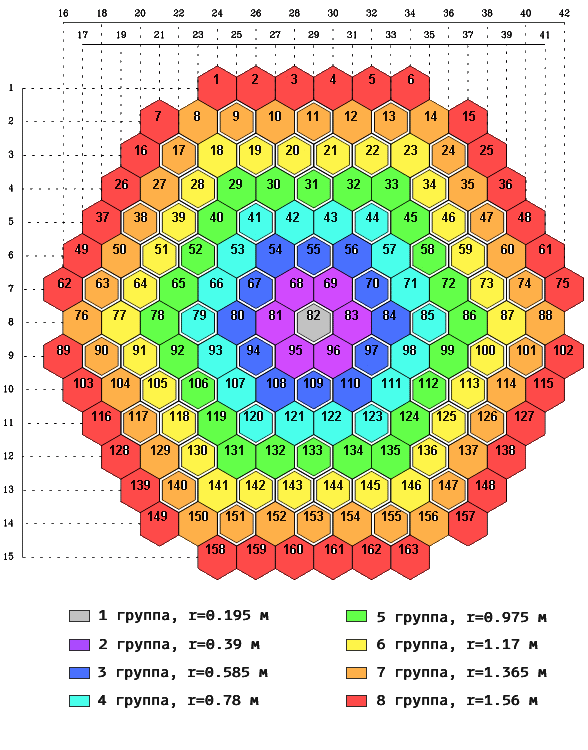
\includegraphics[scale=0.7]{treton_cells.png}
		\caption{Картограмма ячеек моделируемой АЗ для расчетного кода «ТРЕТОН» 
				 и их разбиение на группы по радиусу}
		\label{pic:treton-kartogramma}
	\end{center}
\end{figure}


Для каждой зоны были расчитаны тепловыделения, нормируя на соответствующие $K_r^i$, $K_z^j$, где $i = \overline{1, 8}$, $j = \overline {1, 30}$.

Распределение $K_r$ по группам было подобрано ориентируясь на следующие зависимости:
\begin{equation}
    K_r(r) \sim J_0(\frac{\xi_0 r}{R_{\text{эфф}}}) \approx - \alpha r^2 + \beta
\end{equation}, распределение коэффициента неравномерности по радиусу в приближении параболической функции
\begin{equation}
    \label{equation:KriNi}
    \sum_{i=1}^{8} K_r^i N_i = N_{\text{ТВС}} \pm 0.01
\end{equation}, где $N_i$ — количество ТВС в $i$-той группе по радиусу – условие нормировки распределения коэффициента неравномерности по радиусу.
Коэффициент $\beta$ параболической функции был подобран из условия, что в центре $K_r(r=0)$ должна быть равна табличному значению $K_r$ из \ref{tabular:data}, коэффициент $\alpha$ для удовлетворения соотношения \ref{equation:KriNi}. Полученные значения распределения коэффициента неравномерности по радиусу для каждой группы представлены в таблице \ref{tabular:Kri}.

\begin{figure}[H]
	\begin{center}
		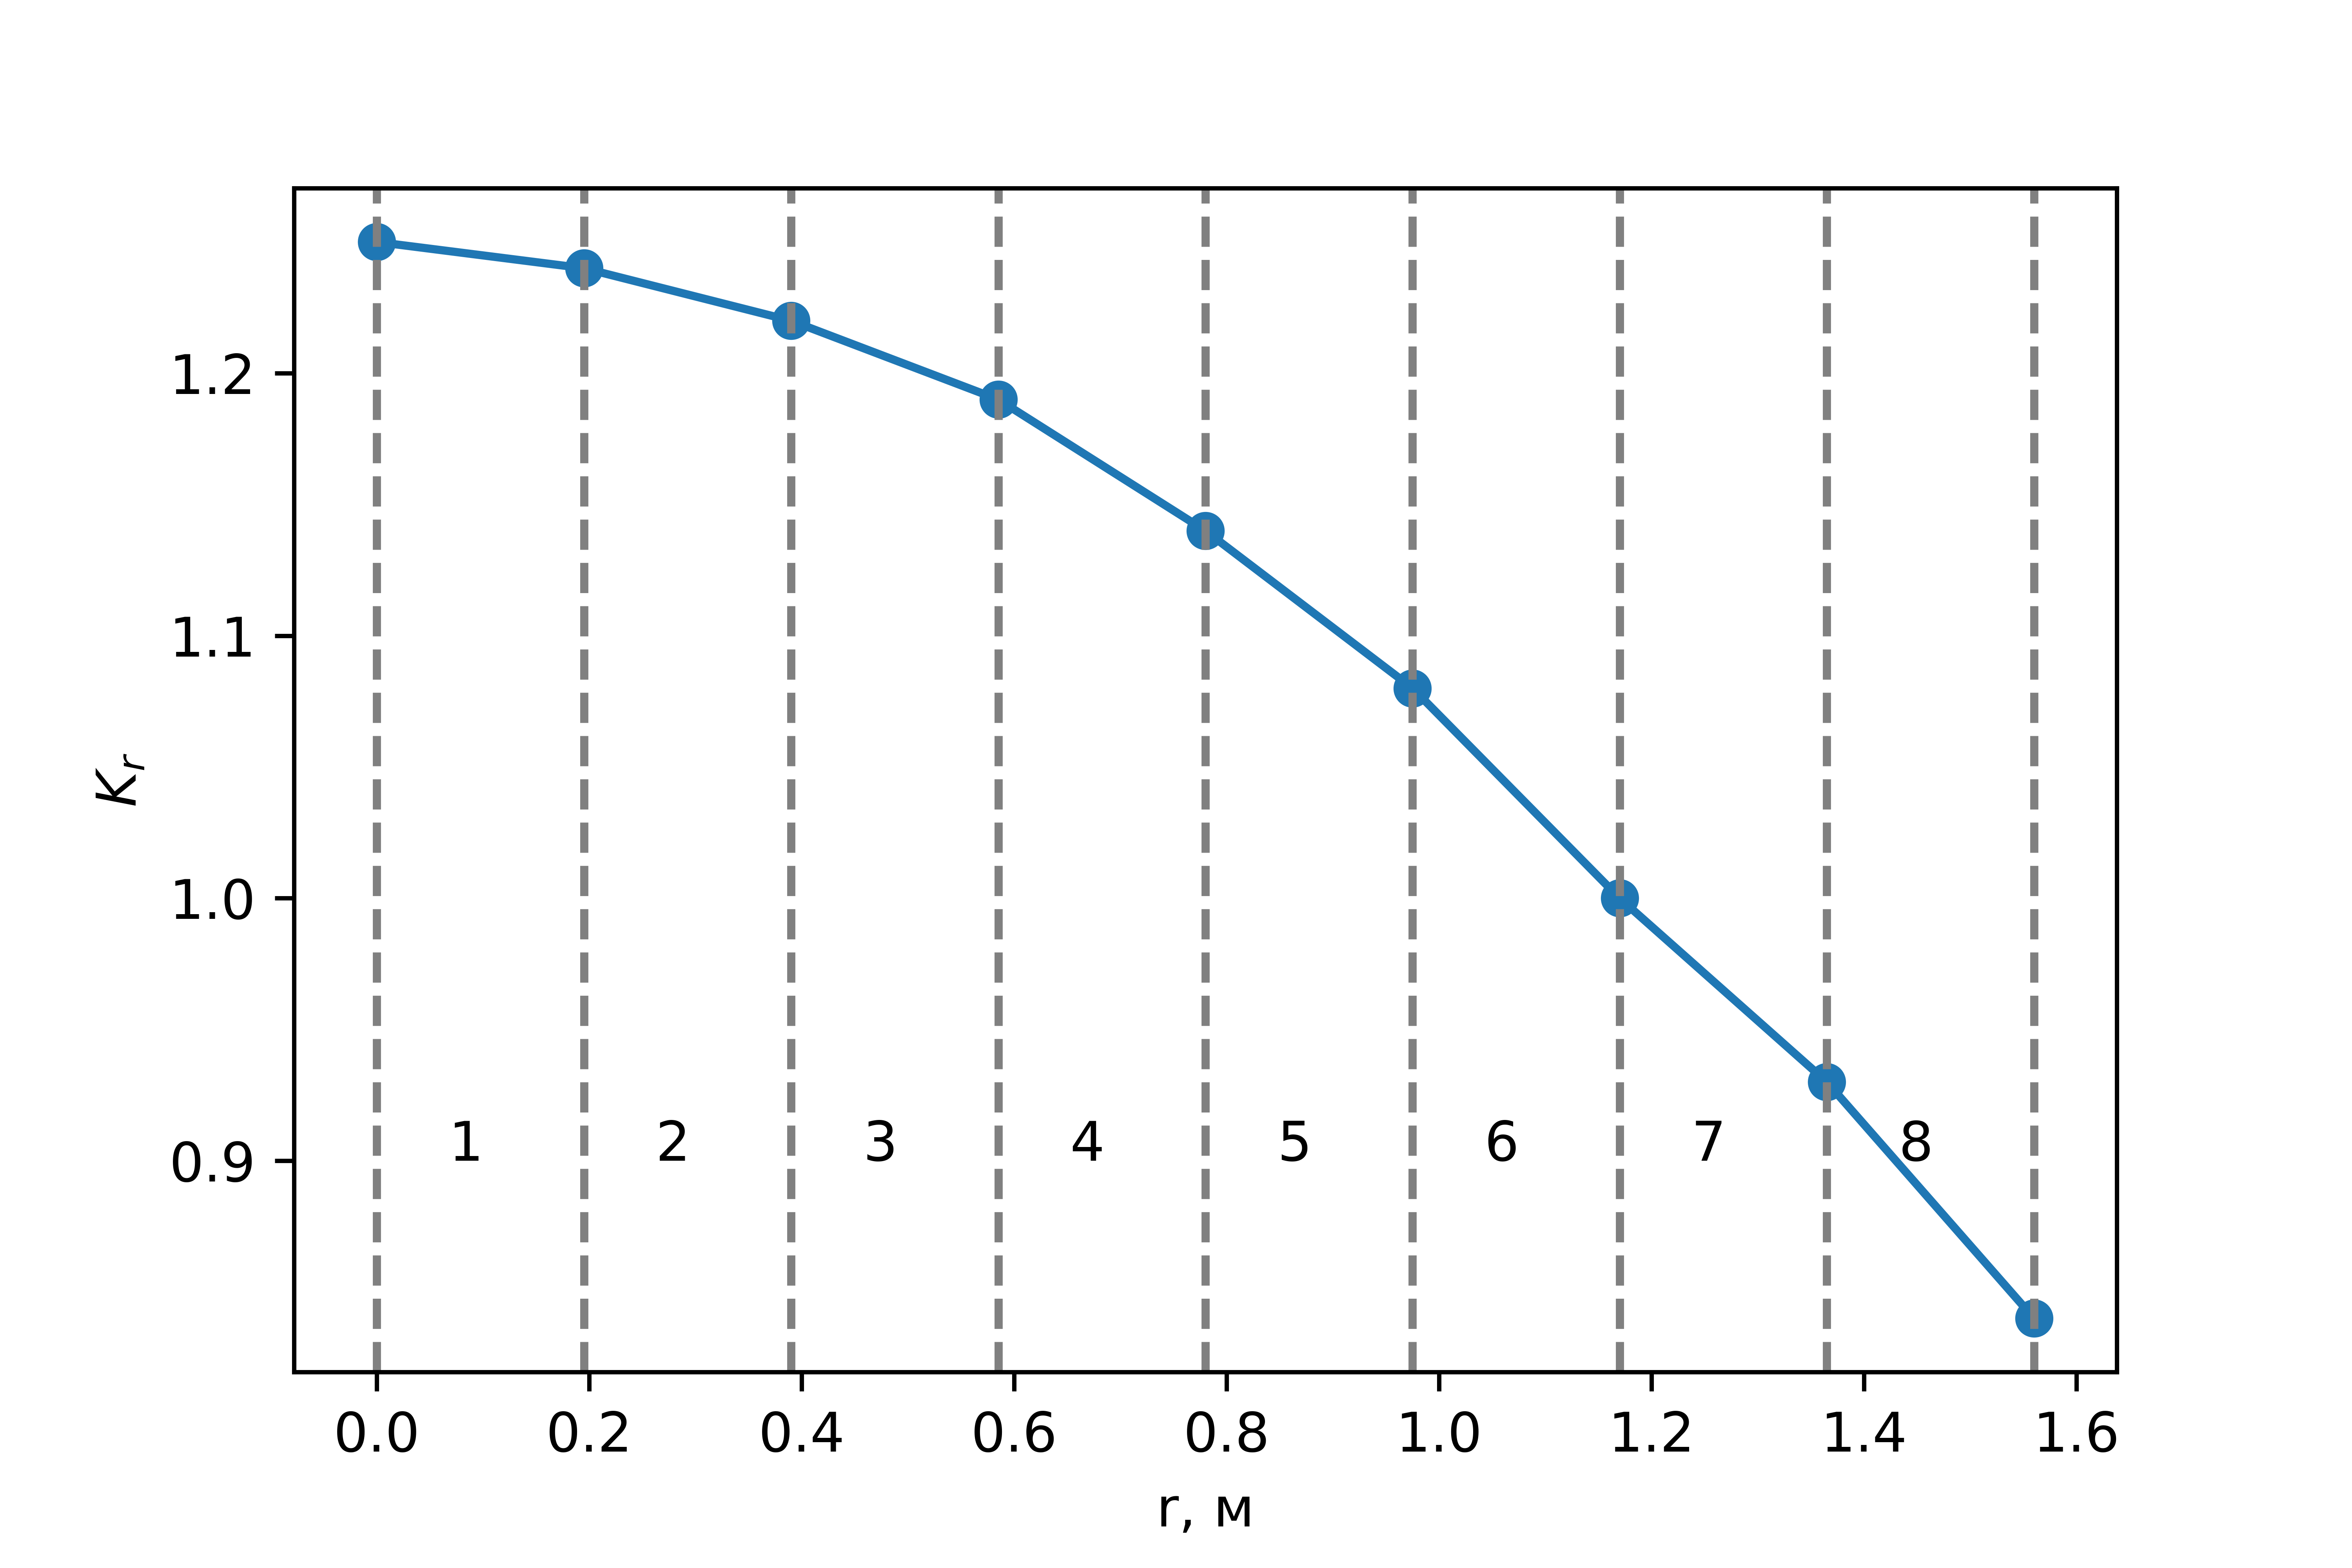
\includegraphics[scale=0.8]{Kr.png}
		\caption{Распределение коэффициента неравномерности по радиусу для восьми групп ТВС}
		\label{pic:Kr}
	\end{center}
\end{figure}

\begin{table}[H]
	\caption{Коэффициент неравномерности энерговыделения по радиусу для групп ТВС}
	\begin{center}
        \begin{tabular}{|l|c|}
        \toprule
         Номер группы & Значение $K_r^i$ \\
         \midrule
         \hline
         1 & 1.24 \\
         \hline
         2 & 1.22 \\
         \hline
         3 & 1.19 \\
         \hline
         4 & 1.14 \\
         \hline
         5 & 1.08 \\
         \hline
         6 & 1.00 \\
         \hline
         7 & 0.93 \\
         \hline
         8 & 0.84 \\
         \bottomrule
		\end{tabular}
		\label{tabular:Kri}
	\end{center}
\end{table}


\noindent Распределение коэффициента неравномерности по высоте $K_z$ определяется как:
\begin{equation}
    K_z(z) = K_z \cos \left( \frac {\pi z} {H_{\text{эфф}}} \right)
\end{equation}
где $z = \overline{-H_{\text{АЗ}} / 2,\  H_{\text{АЗ}} / 2}$ м.


\noindent Распределение $K_z$ по высоте представлено на рис \ref{pic:Kz}


\begin{figure}[H]
	\begin{center}
		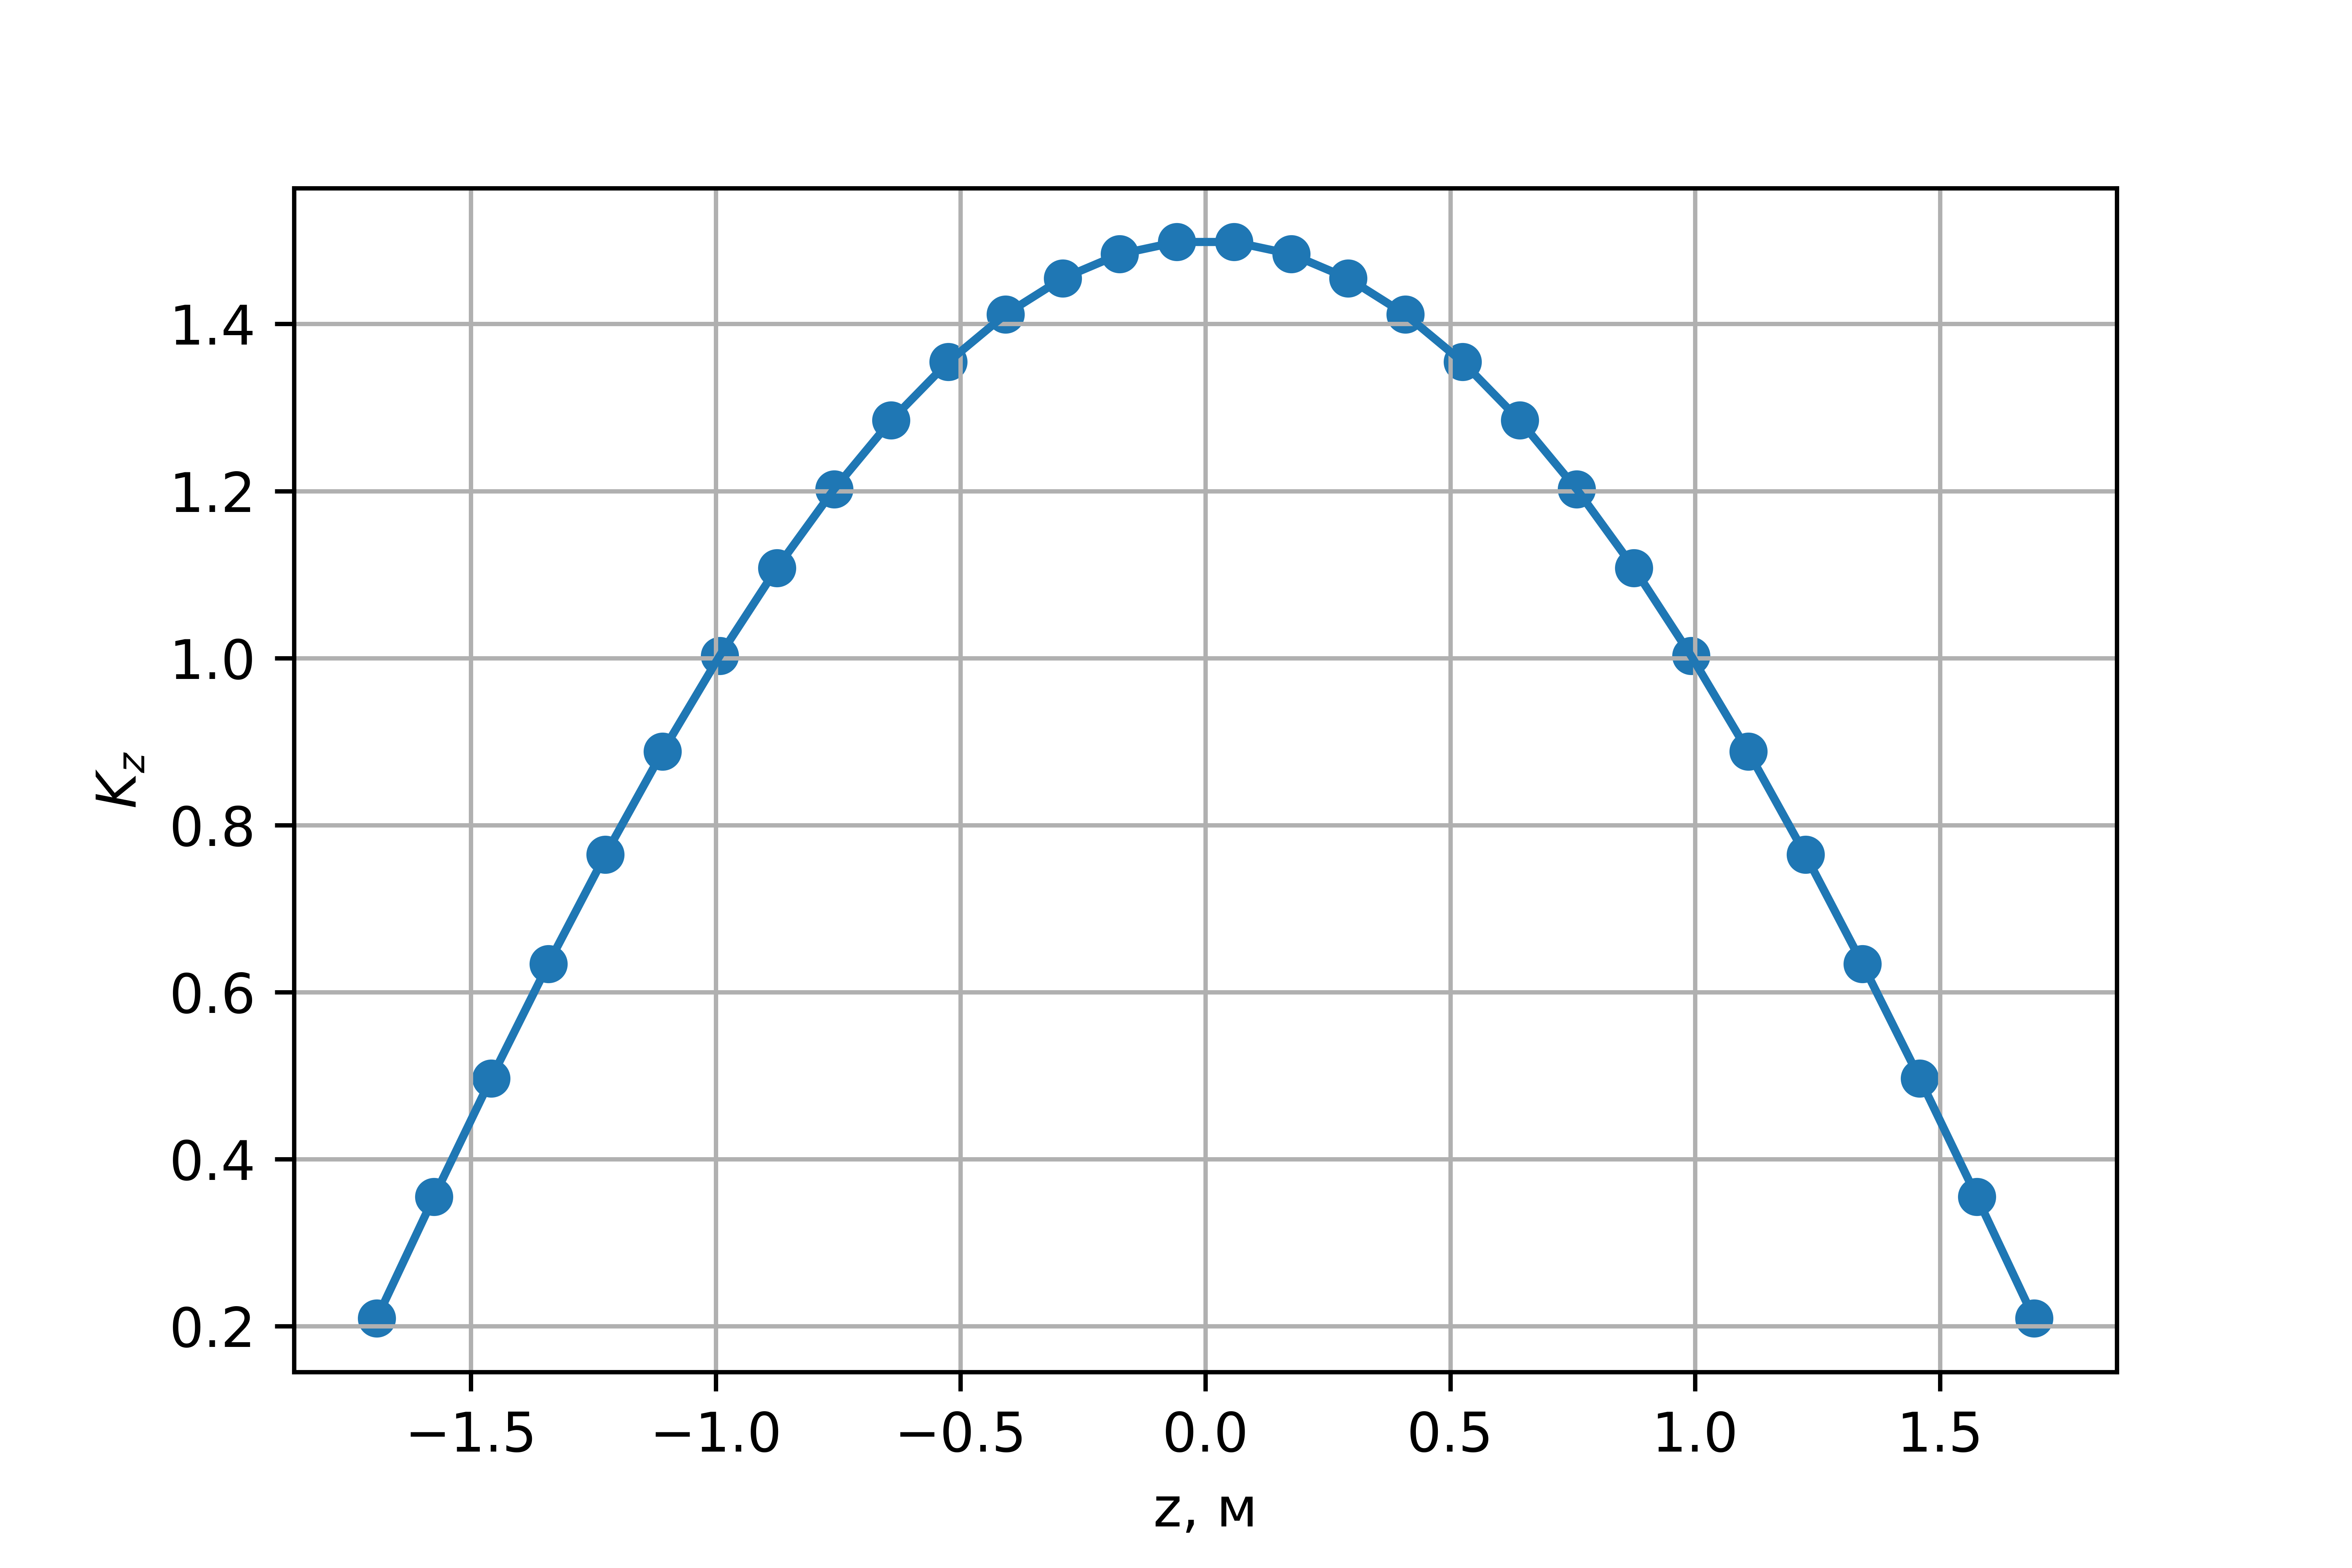
\includegraphics[scale=0.8]{Kz.png}
		\caption{Распределение коэффициента неравномерности по высоте активной зоны}
		\label{pic:Kz}
	\end{center}
\end{figure}


Из полученных распределений $K_r$, $K_z$ было определено распределение тепловыделения для всех групп расчетных элементов
\begin{align}
    \label{equation:Qzr}
    Q(z, r) &= K_z(z)K_r(r)\frac{Q_{\text{теп}}}{N_{\text{ТВС}} \cdot 30} \\
            &= K_r(r) K_z \cos \left( \frac{\pi z}{H_{\text{эфф}}} \right) \frac{Q_{\text{теп}}}{N_{\text{ТВС}} 30}
\end{align}

На основе соотношения \ref{equation:Qzr} был сформирован входной файл \texttt{Q6.txt} с тепловыделением для всех расчетных элементов в соответствии с картограммой \ref{pic:treton-kartogramma}

Далее были проведены калибровочные расчеты для определения входных параметров файла \texttt{THEHYCO.INI}, соответствующих проектируемой РУ. Основным критерием выбора параметров было соответсвие вычисленному программой «ТРЕТОН» расходу полученному ранее в рамках теплофизического расчета.

Таким образом расчетным кодом было получено значение расхода $G_{\text{расч}} = (1.570 \pm 0.016) \cdot 10^4\  \frac{\text{кг}}{\text{с}}$, что соответствует полученному ранее значению $G_{\text{реак}} = 1.579 \cdot 10^4\ \frac{\text{кг}}{\text{с}}$ в пределах погрешности. 
Значения входных параметров файла \texttt{THETHYCO.INI}, при которых достигнут такой расход приведены в таблице \ref{tabular:thethyco_nominal}

\begin{table}[H]
    \caption{Входные параметры расчета при номинальном режиме работы}
    \begin{center}
        \begin{tabular}{|l|c|}
        \toprule
        Параметр & Значение \\
        \midrule
        \hline
        Шаг твэлов, мм & 12.75 \\ 
        \hline
        Поперечный размер расчетной области, м & 0.241 \\
        \hline
        Продольный размер расчетной области, м & 0.118 \\
        \hline
        Кол-во твэлов в ТВС, шт & 317 \\
        \hline
        Расчетный дисбаланс & 0.005 \\
        \hline
        Входное давление, Па & 15800000 \\
        \hline
        Выходное давление, Па & 15686938 \\
        \bottomrule
        \end{tabular}
		\label{tabular:thehyco_nominal}
    \end{center}
\end{table}

% TODO: табличка с параметрами THEHYCO.INI по разделам с именами

% \begin{table}[H]
% 	\caption{wow}
% 	\begin{center}
%         \begin{tabular}{|l|c|}
%         \toprule
%          Раздел RodList & \\
%          \midrule
%          \hline
%          tmp=0.75 3.86 4.25 4.55 & разбиение твэлов на контрольные объемы, указаны радиусы центрального отверстия твэла, границы топливного столба, центра оболочки, внешней границы оболочки. мм\\
%          \hline
%          $\texttt{s_mesh}$=12.75 & шаг твэлов, мм \\
%          \hline
%          d\_mesh=9.1 & диаметр твэла, мм \\
%          \hline
%         %  $\texttt{R_contact}$=0.00024 & контактное сопротивление толиво-оболочка, $\text{м}^2 \cdot \text{К} / \text{Вт}$ \\
%         %  \hline
%          Раздел HEATandHYDROlist & \\
%          \midrule
%          \texttt{dr}=0.241 & поперечный размер расчетной области, м\\
%          \hline
%          \texttt{dz}=0.118 & продольный размер расчетной области, м\\
%          \hline
%          $\texttt{n_RodsInTVS}$ =317 & количество твэлов в ТВС \\
%          \hline
%          \texttt{Disbalance}=0.001 & расчетный дисбаланс \\
%          \hline
%          $\texttt{p_input}$=15800000 & входное давление, Па \\
%          \hline
%          $\texttt{p_output}$=15691054 & выходное давление,  Па \\
%          \bottomrule
% 		\end{tabular}
% 		\label{tabular:thehyco_nominal}
% 	\end{center}
% \end{table}

На основе описанных входных параметров был произведен расчет с шагом по времени $dt=0.0005$ для 100 итераций. По результату расчета были построены зависимости основных теплогидравлических параметров и сопоставлены со значениями, полученными в теплофизческом расчете.

По итогам расчета на основе результатов файла \texttt{t\_tepl.dat} была построено распределение температуры теплоносителя по высоте активной зоны, усредненное по всем расчетным элементам. График распределения вместе с распределением теплоносителя по высоте, рассчитанном в рамках теплофизического расчета представлен на рисунке \ref{pic:treton-t-tepl-compare-teplofiz}.

\begin{figure}[H]
	\begin{center}
		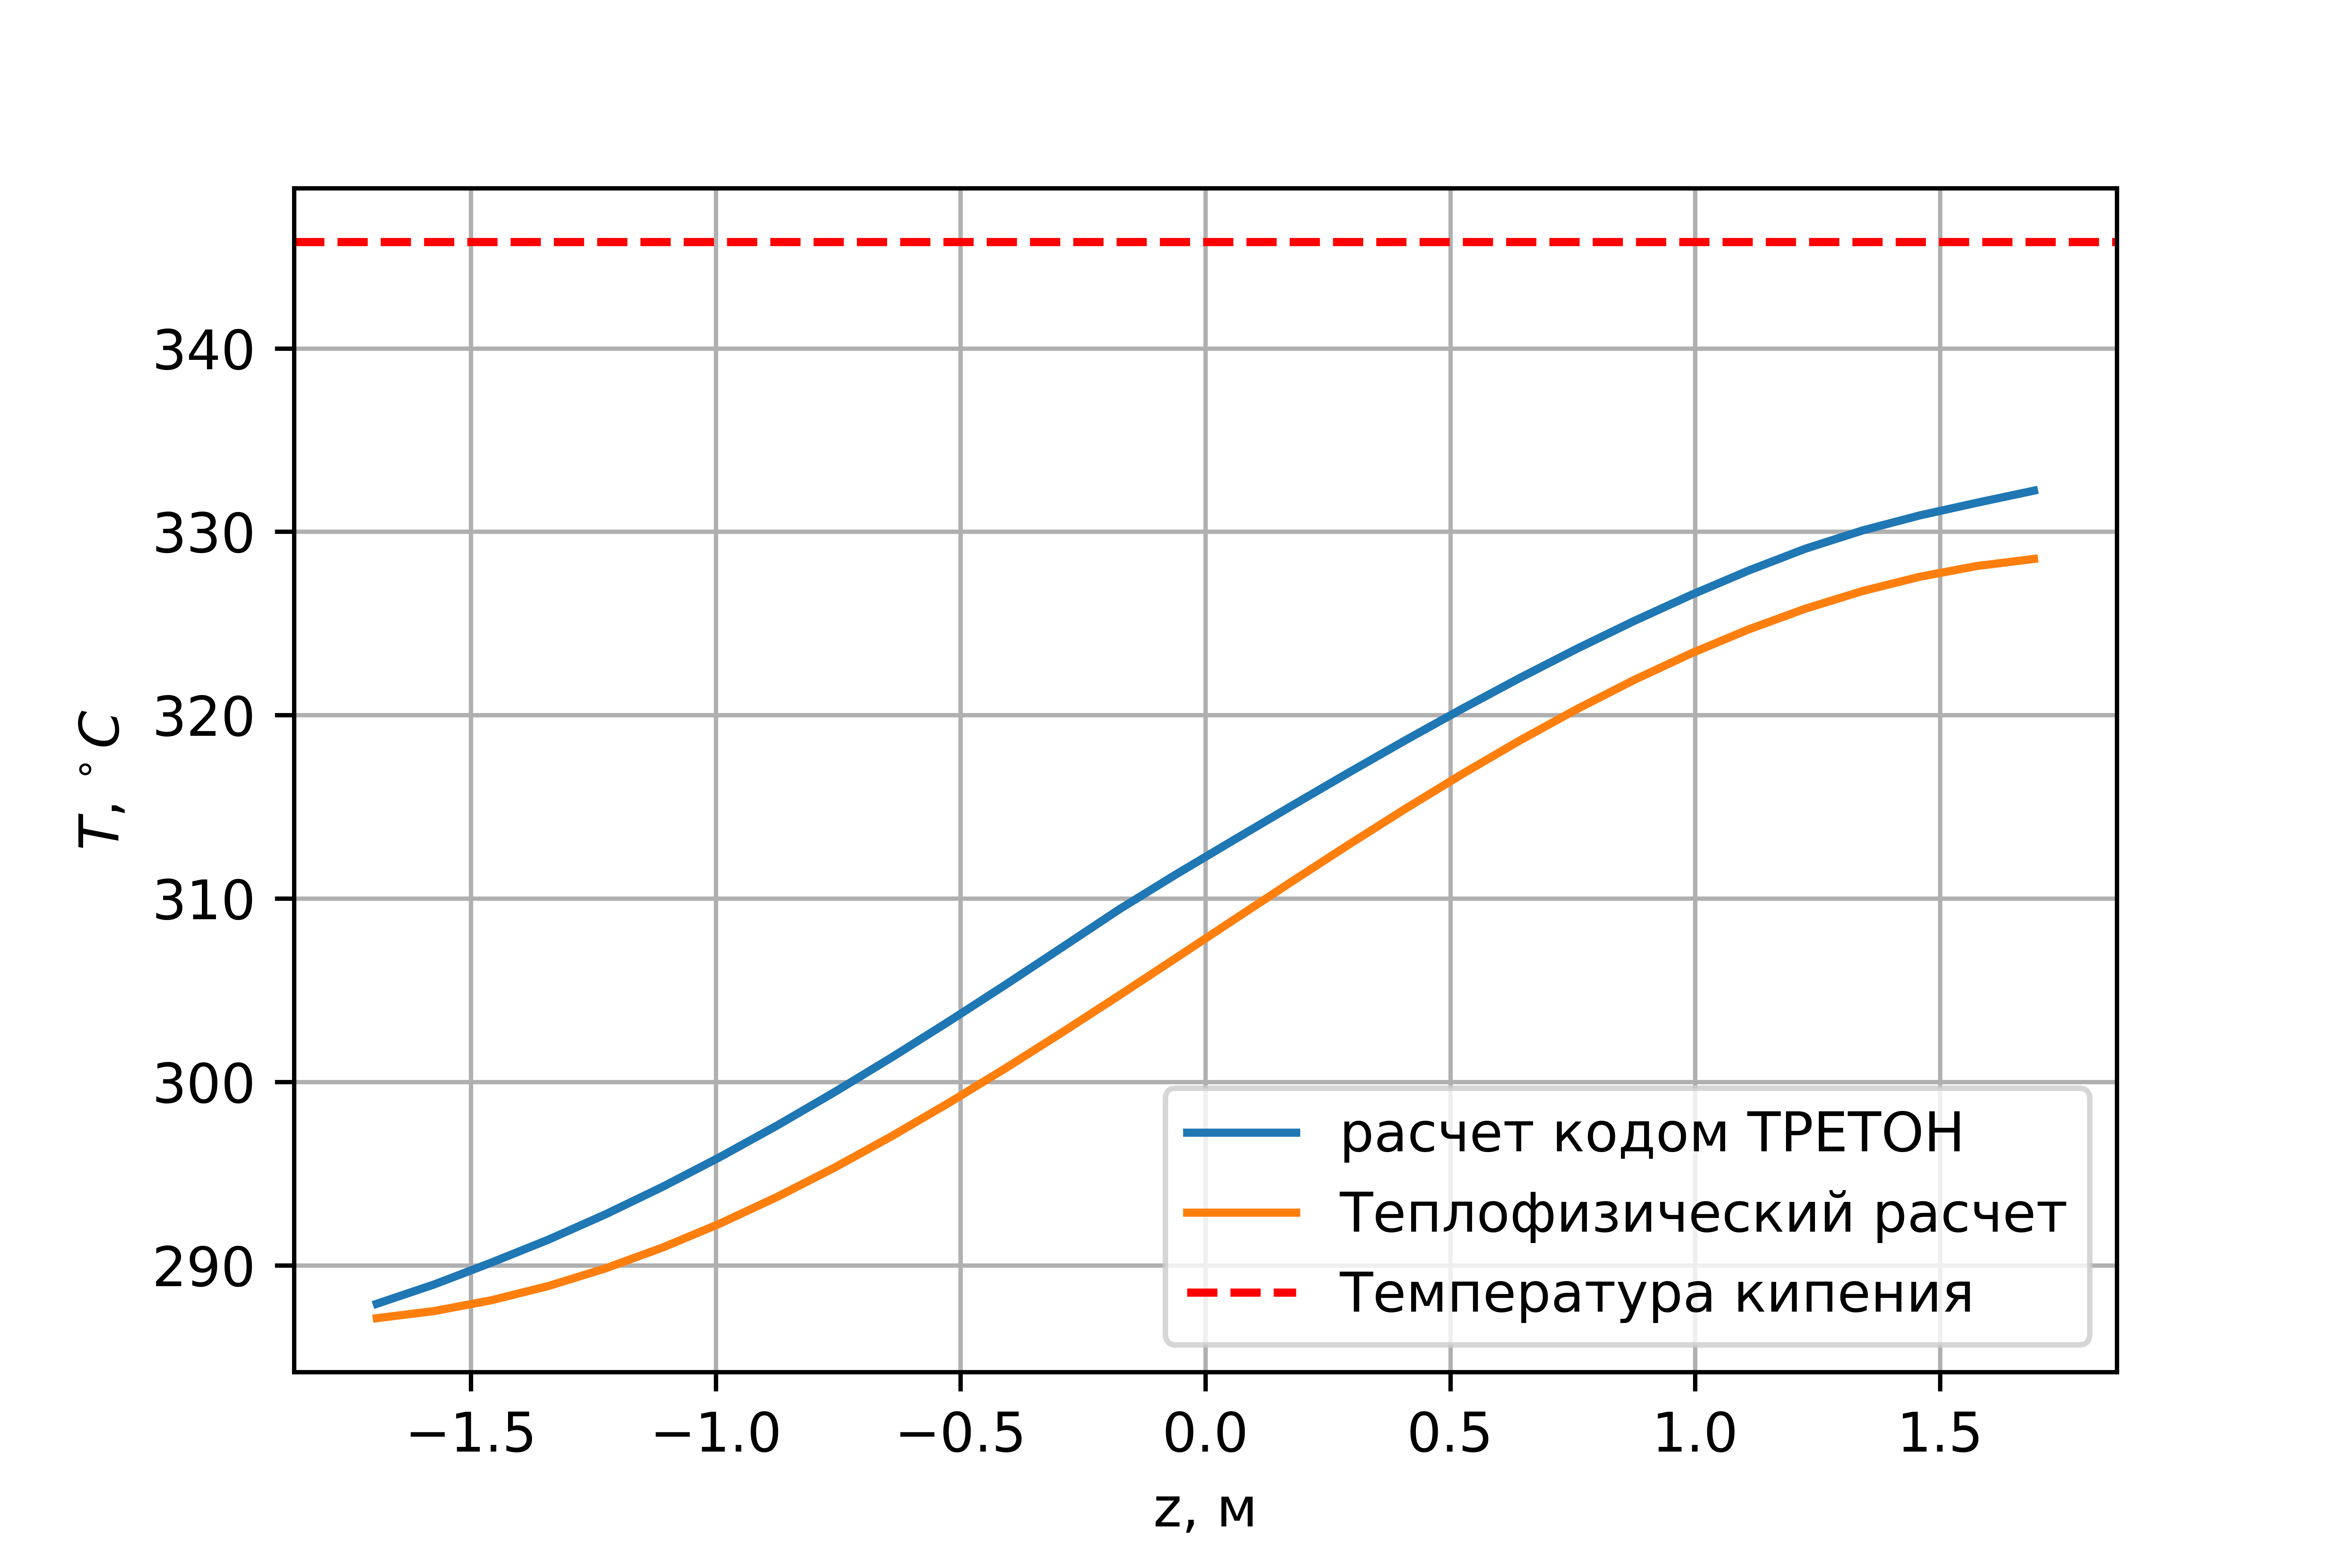
\includegraphics{treton_nominal_t_z.png}
		\caption{Распределение температуры теплоносителя по высоте}
		\label{pic:treton-t-tepl-compare-teplofiz} % название для ссылок внутри кода
	\end{center}
\end{figure}

Из рис \ref{pic:treton-t-tepl-compare-teplofiz} видно, что среднеквадратичная ошибка составляет $\Delta {T_{\text{теп}}} = 3.6 ^\circ C$. Несовпадение результатов обусловлено отличием среднего коэффициента теплоемкости рассчитываемого в ТРЕТОН с результатом теоретического расчета. Отсюда мы можем сделать вывод о соответствии полученных результатов ранее рассчитанным в рамках приемлемой погрешности.

Для номинального режима работы реактора были построены распределения температуры теплоносителя по высоте для каждой рассматриваемой групп и для кассеты, с максимальной температурой на выходе из активной зоны. Распределения представлены на рисунках \ref{pic:treton-t-tepl-nominal-by-r}, \ref{pic:treton-t-tepl-nominal-max}. Несовпадение зависимостей для температуры внешней оболочки обусловлено описанным ранее несоответствием среднего коэффициента теплоемкости.

\begin{figure}[H]
	\begin{center}
		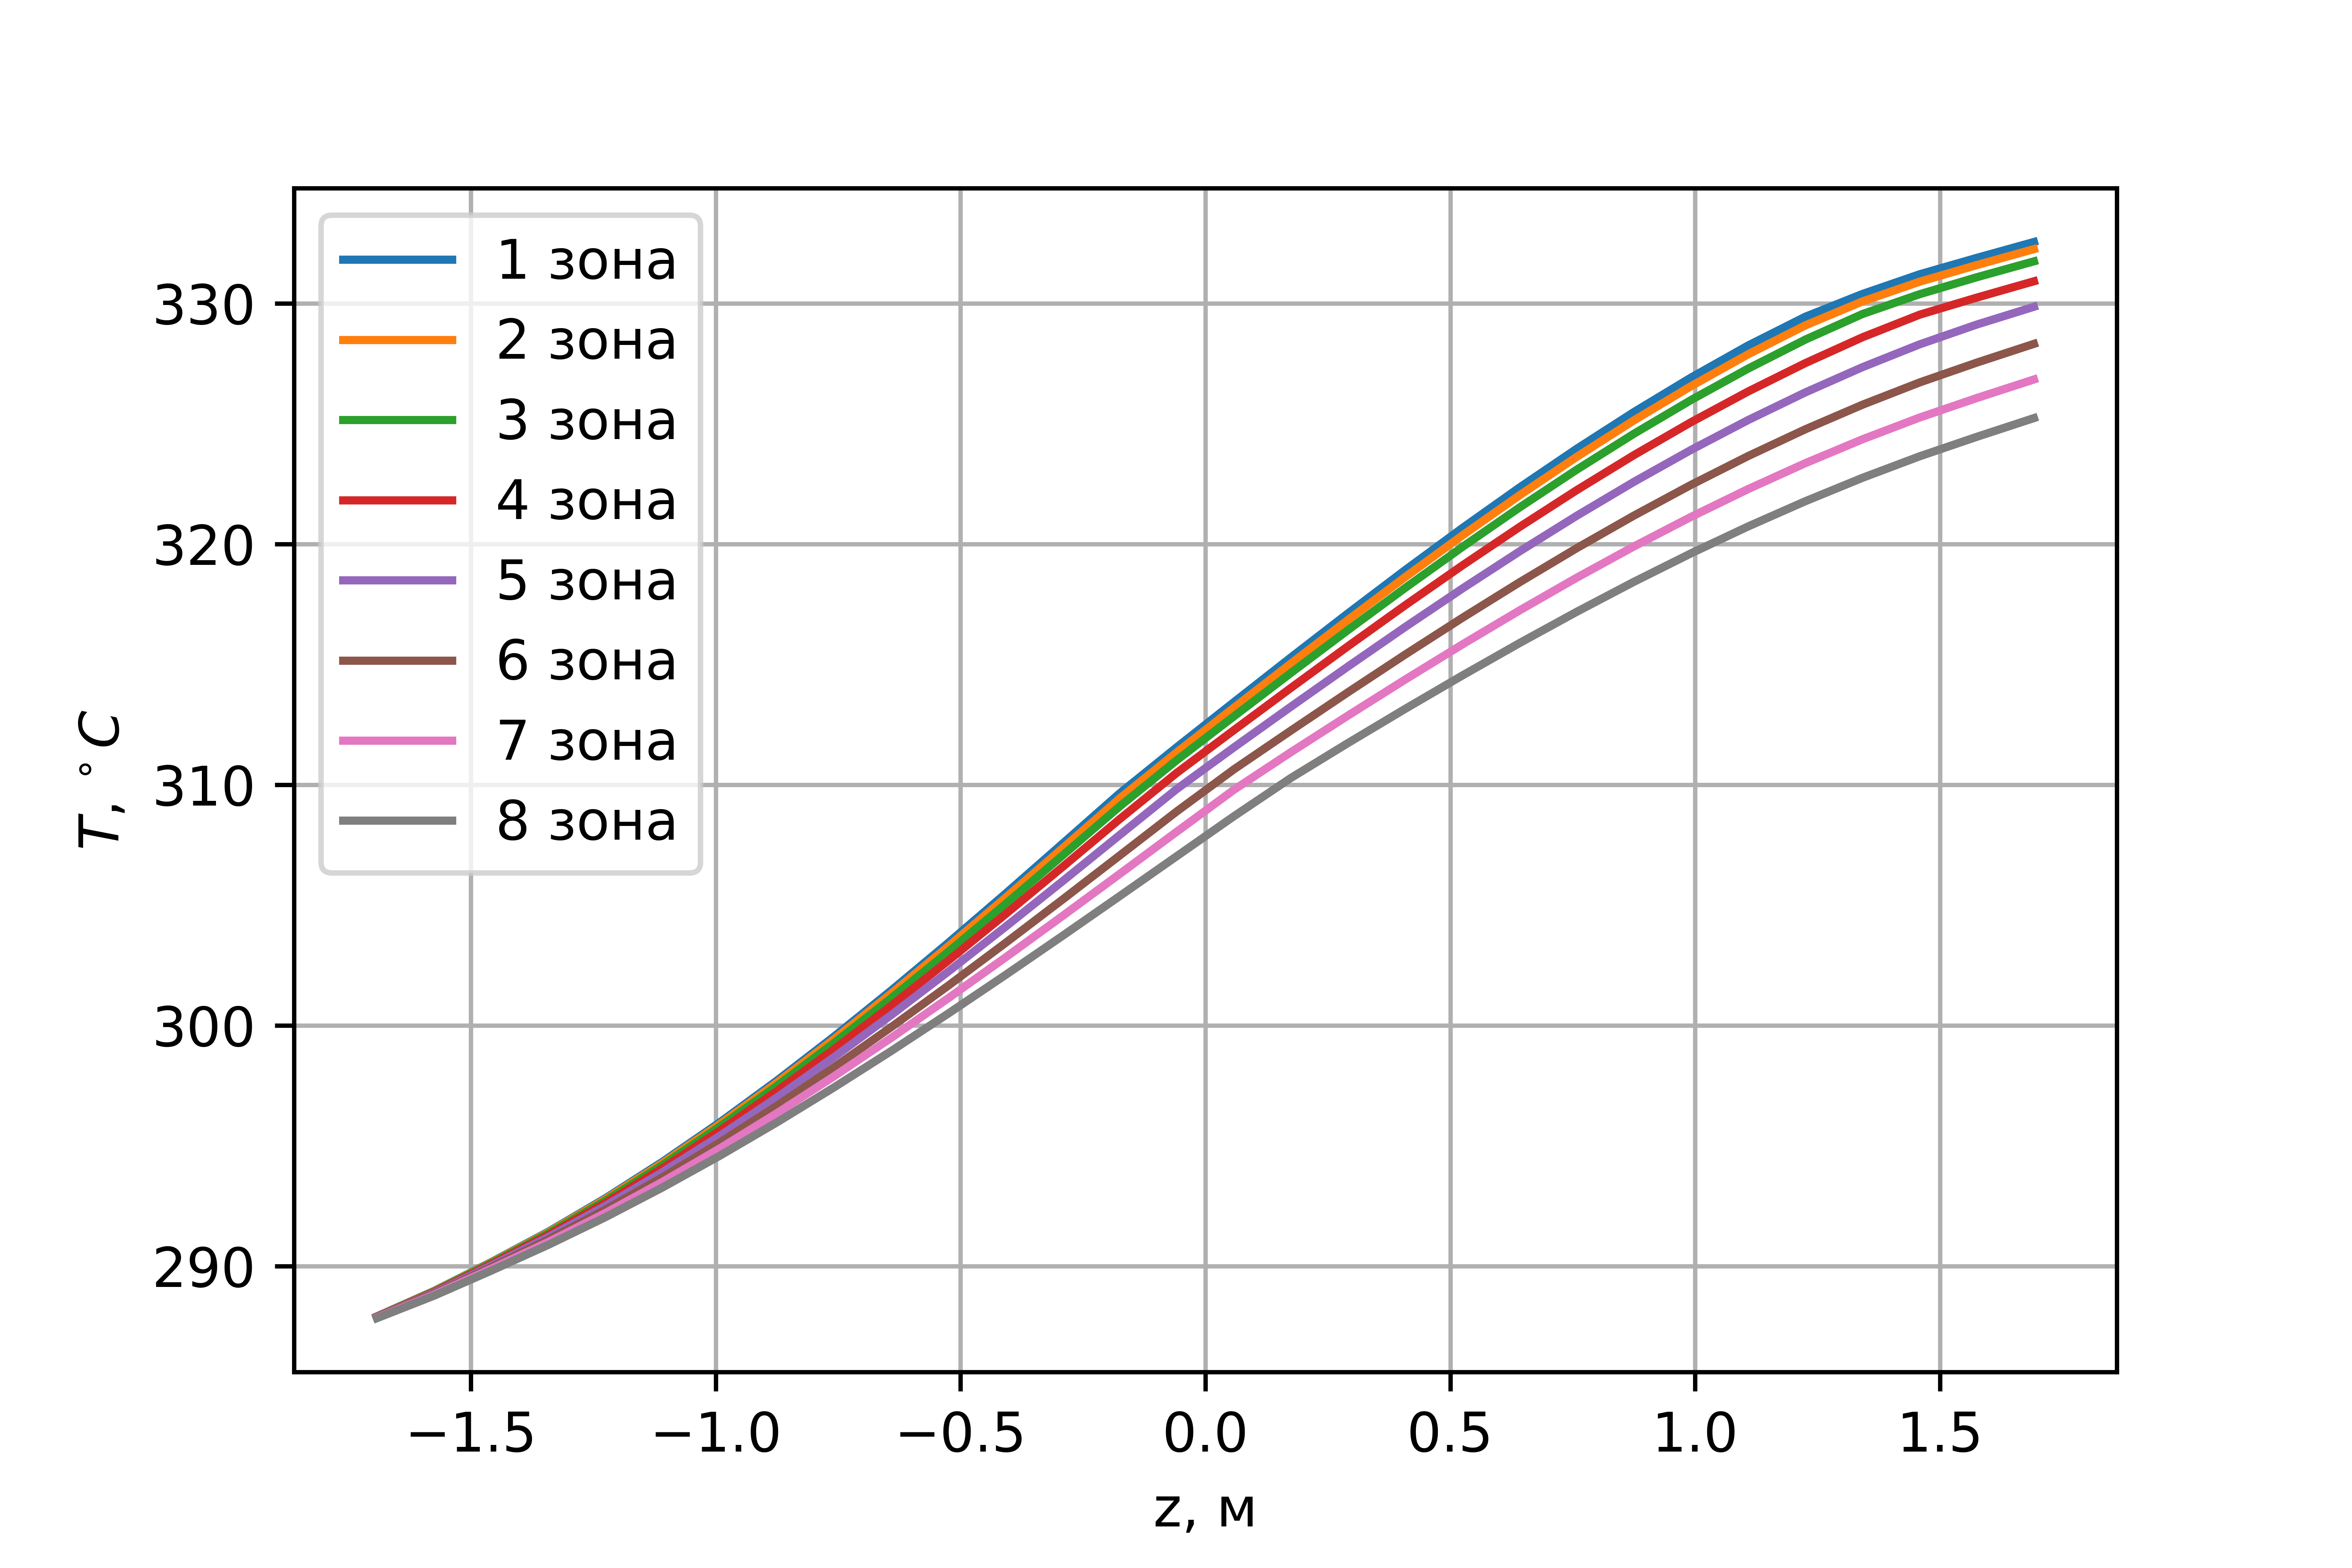
\includegraphics{treton_nominal_t_z_by_r.png}
		\caption{Распределение температуры теплоносителя по высоте для каждой зоны по радиусу}
		\label{pic:treton-t-tepl-nominal-by-r} % название для ссылок внутри кода
	\end{center}
\end{figure}

\begin{figure}[H]
	\begin{center}
		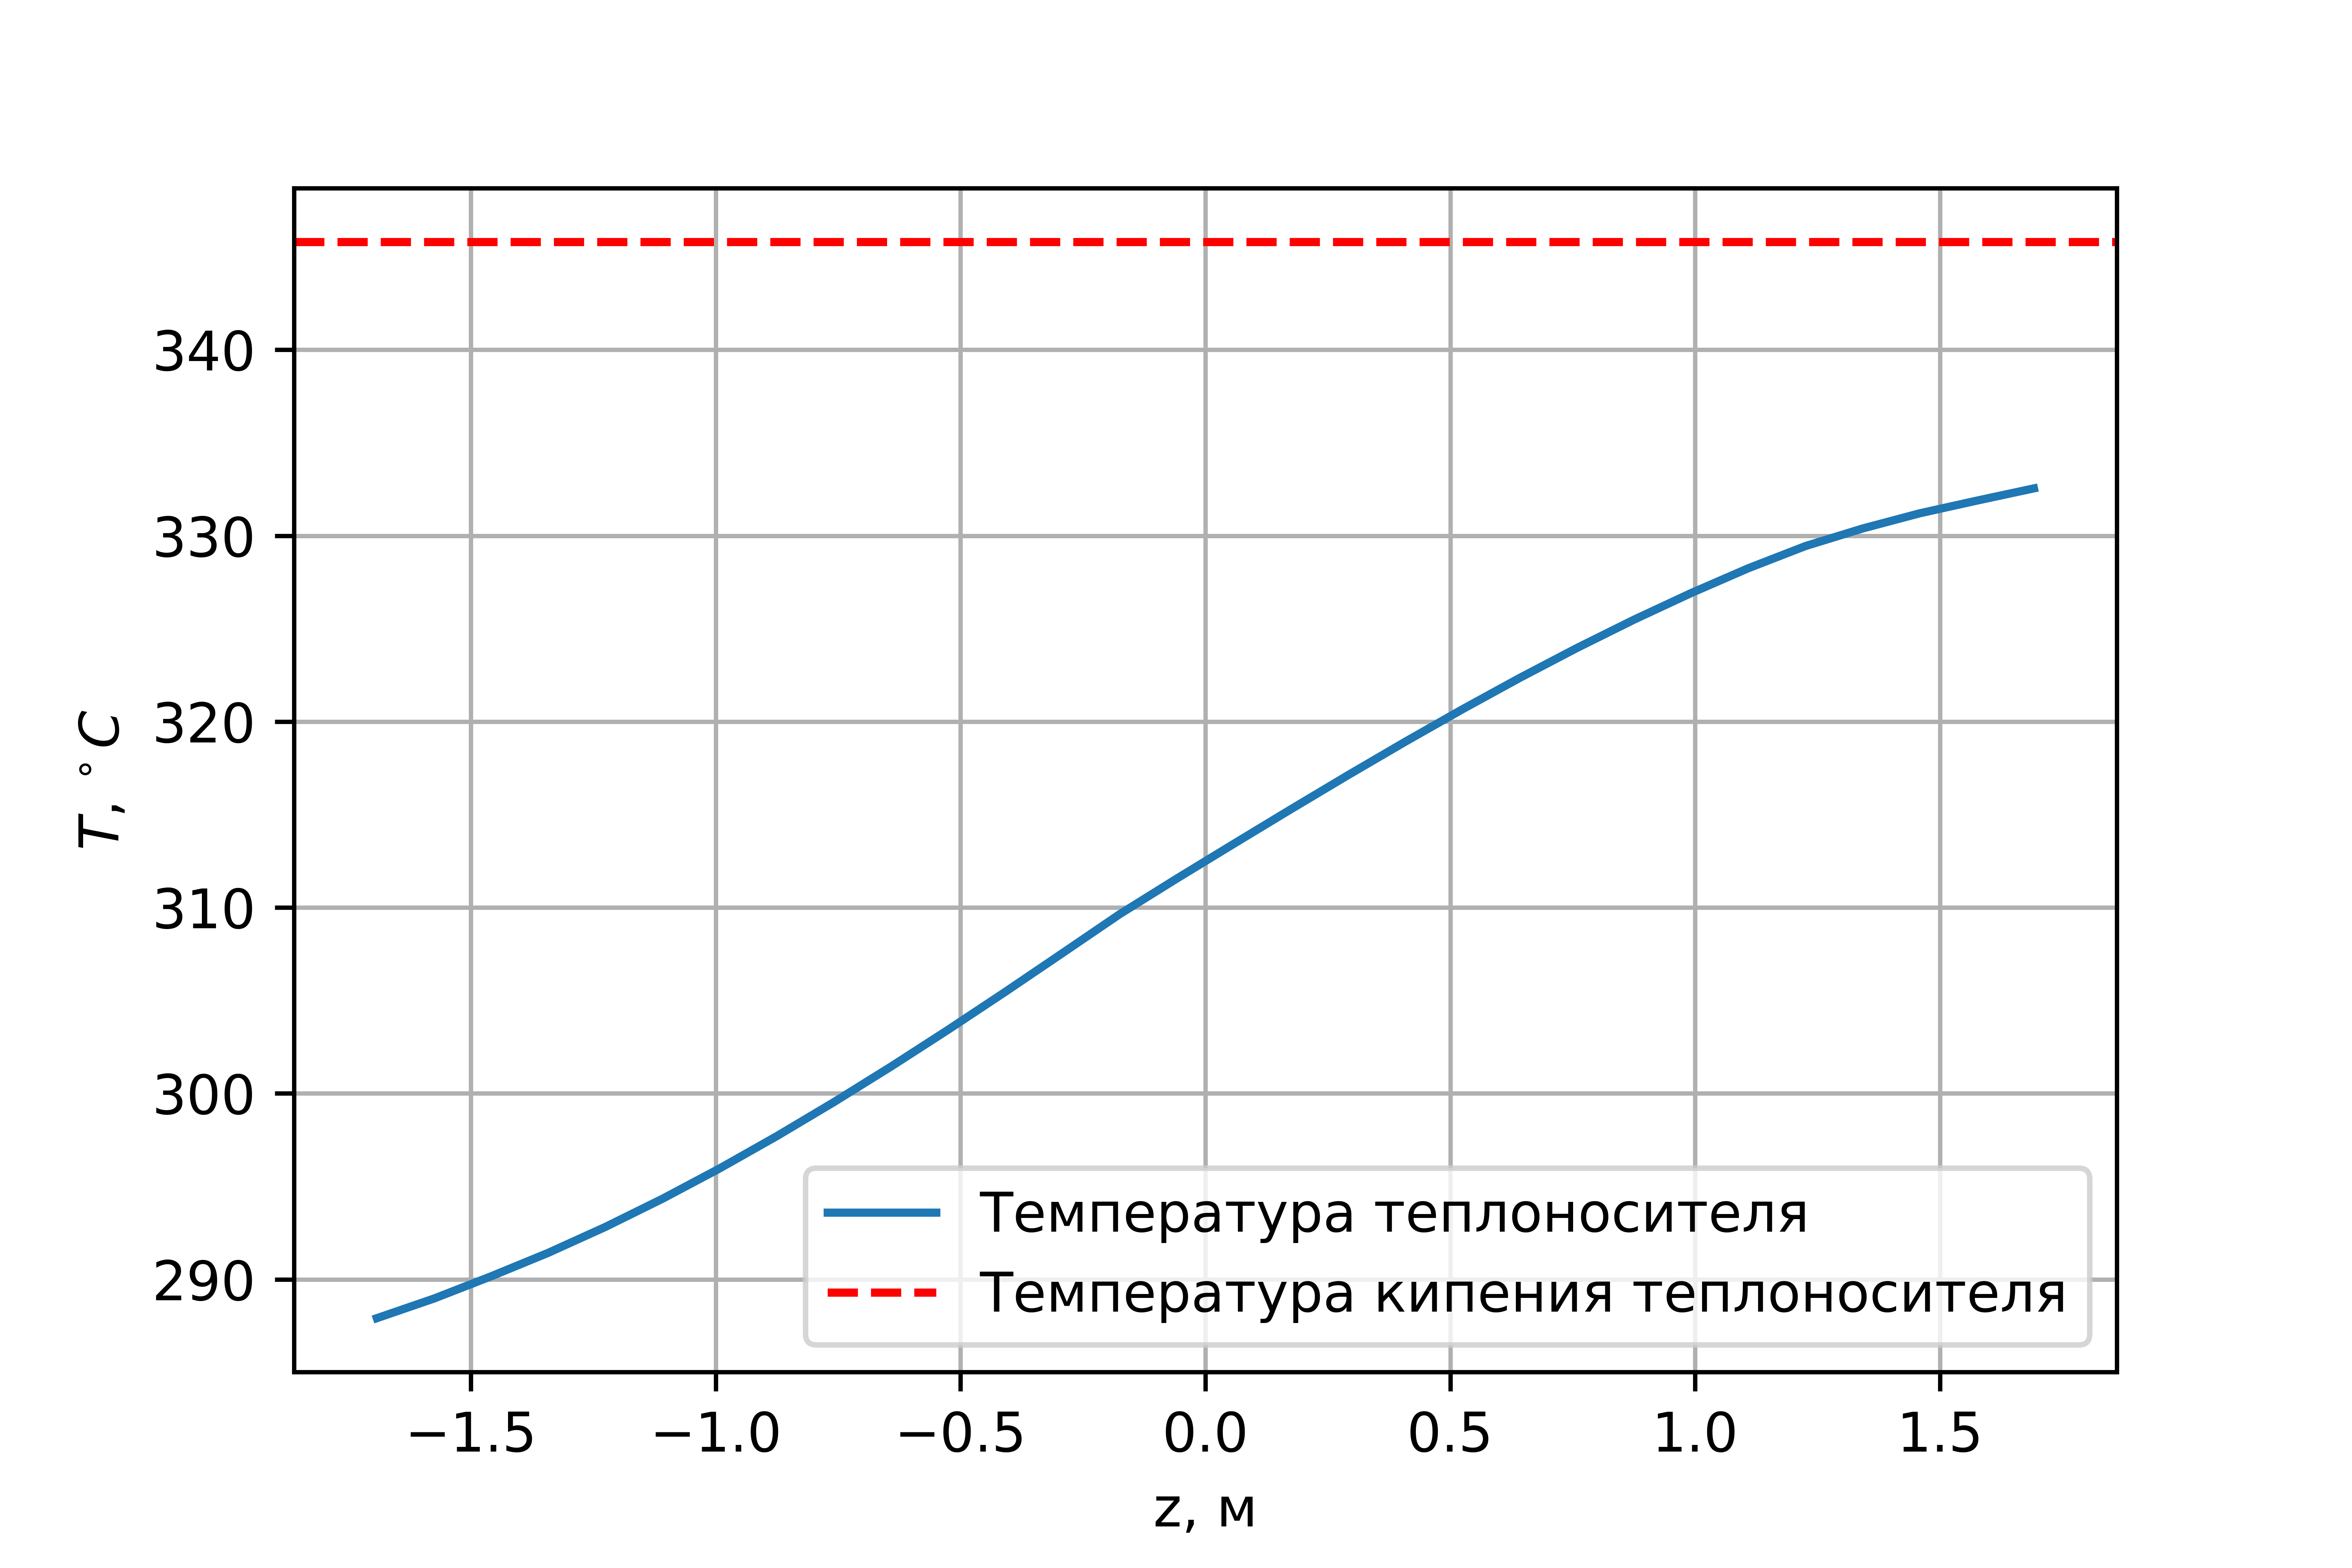
\includegraphics{treton_nominal_t_z_max.png}
		\caption{Распределение температуры теплоносителя по высоте для кассеты с максимальной температурой на вызоде из АЗ}
		\label{pic:treton-t-tepl-nominal-max} % название для ссылок внутри кода
	\end{center}
\end{figure}

 Из \ref{pic:treton-t-tepl-nominal-max} видно, что максимальная температура теплоносителя $T_{\text{тепл} \text{Ном}}^{\max} = 332.5 ^\circ C$.
 При рассматриваемом давлении в активной зоне 15.8 МПа температура кипения теплоносителя составляет $346.5\ ^\circ C$, отсюда следует что запас до кипения составляет $13.65 ^\circ C$

 Для топлива были получены распределения температуры топлива по высоте активной зоны для ячейки с максимальной температурой топлива в центре АЗ и распределение температуры топлива по высоте АЗ для всех групп по радиусу. Зависимости представлены на рисунках \ref{pic:treton-t-fuel-nominal-max}, \ref{pic:treton-t-fuel-nominal-by-r}. Рассчитанная температура топлива заметно отличается от теплофизического расчета ввиду особенностей задания характеристик материалов входящих в состав топилва.

\begin{figure}[H]
	\begin{center}
		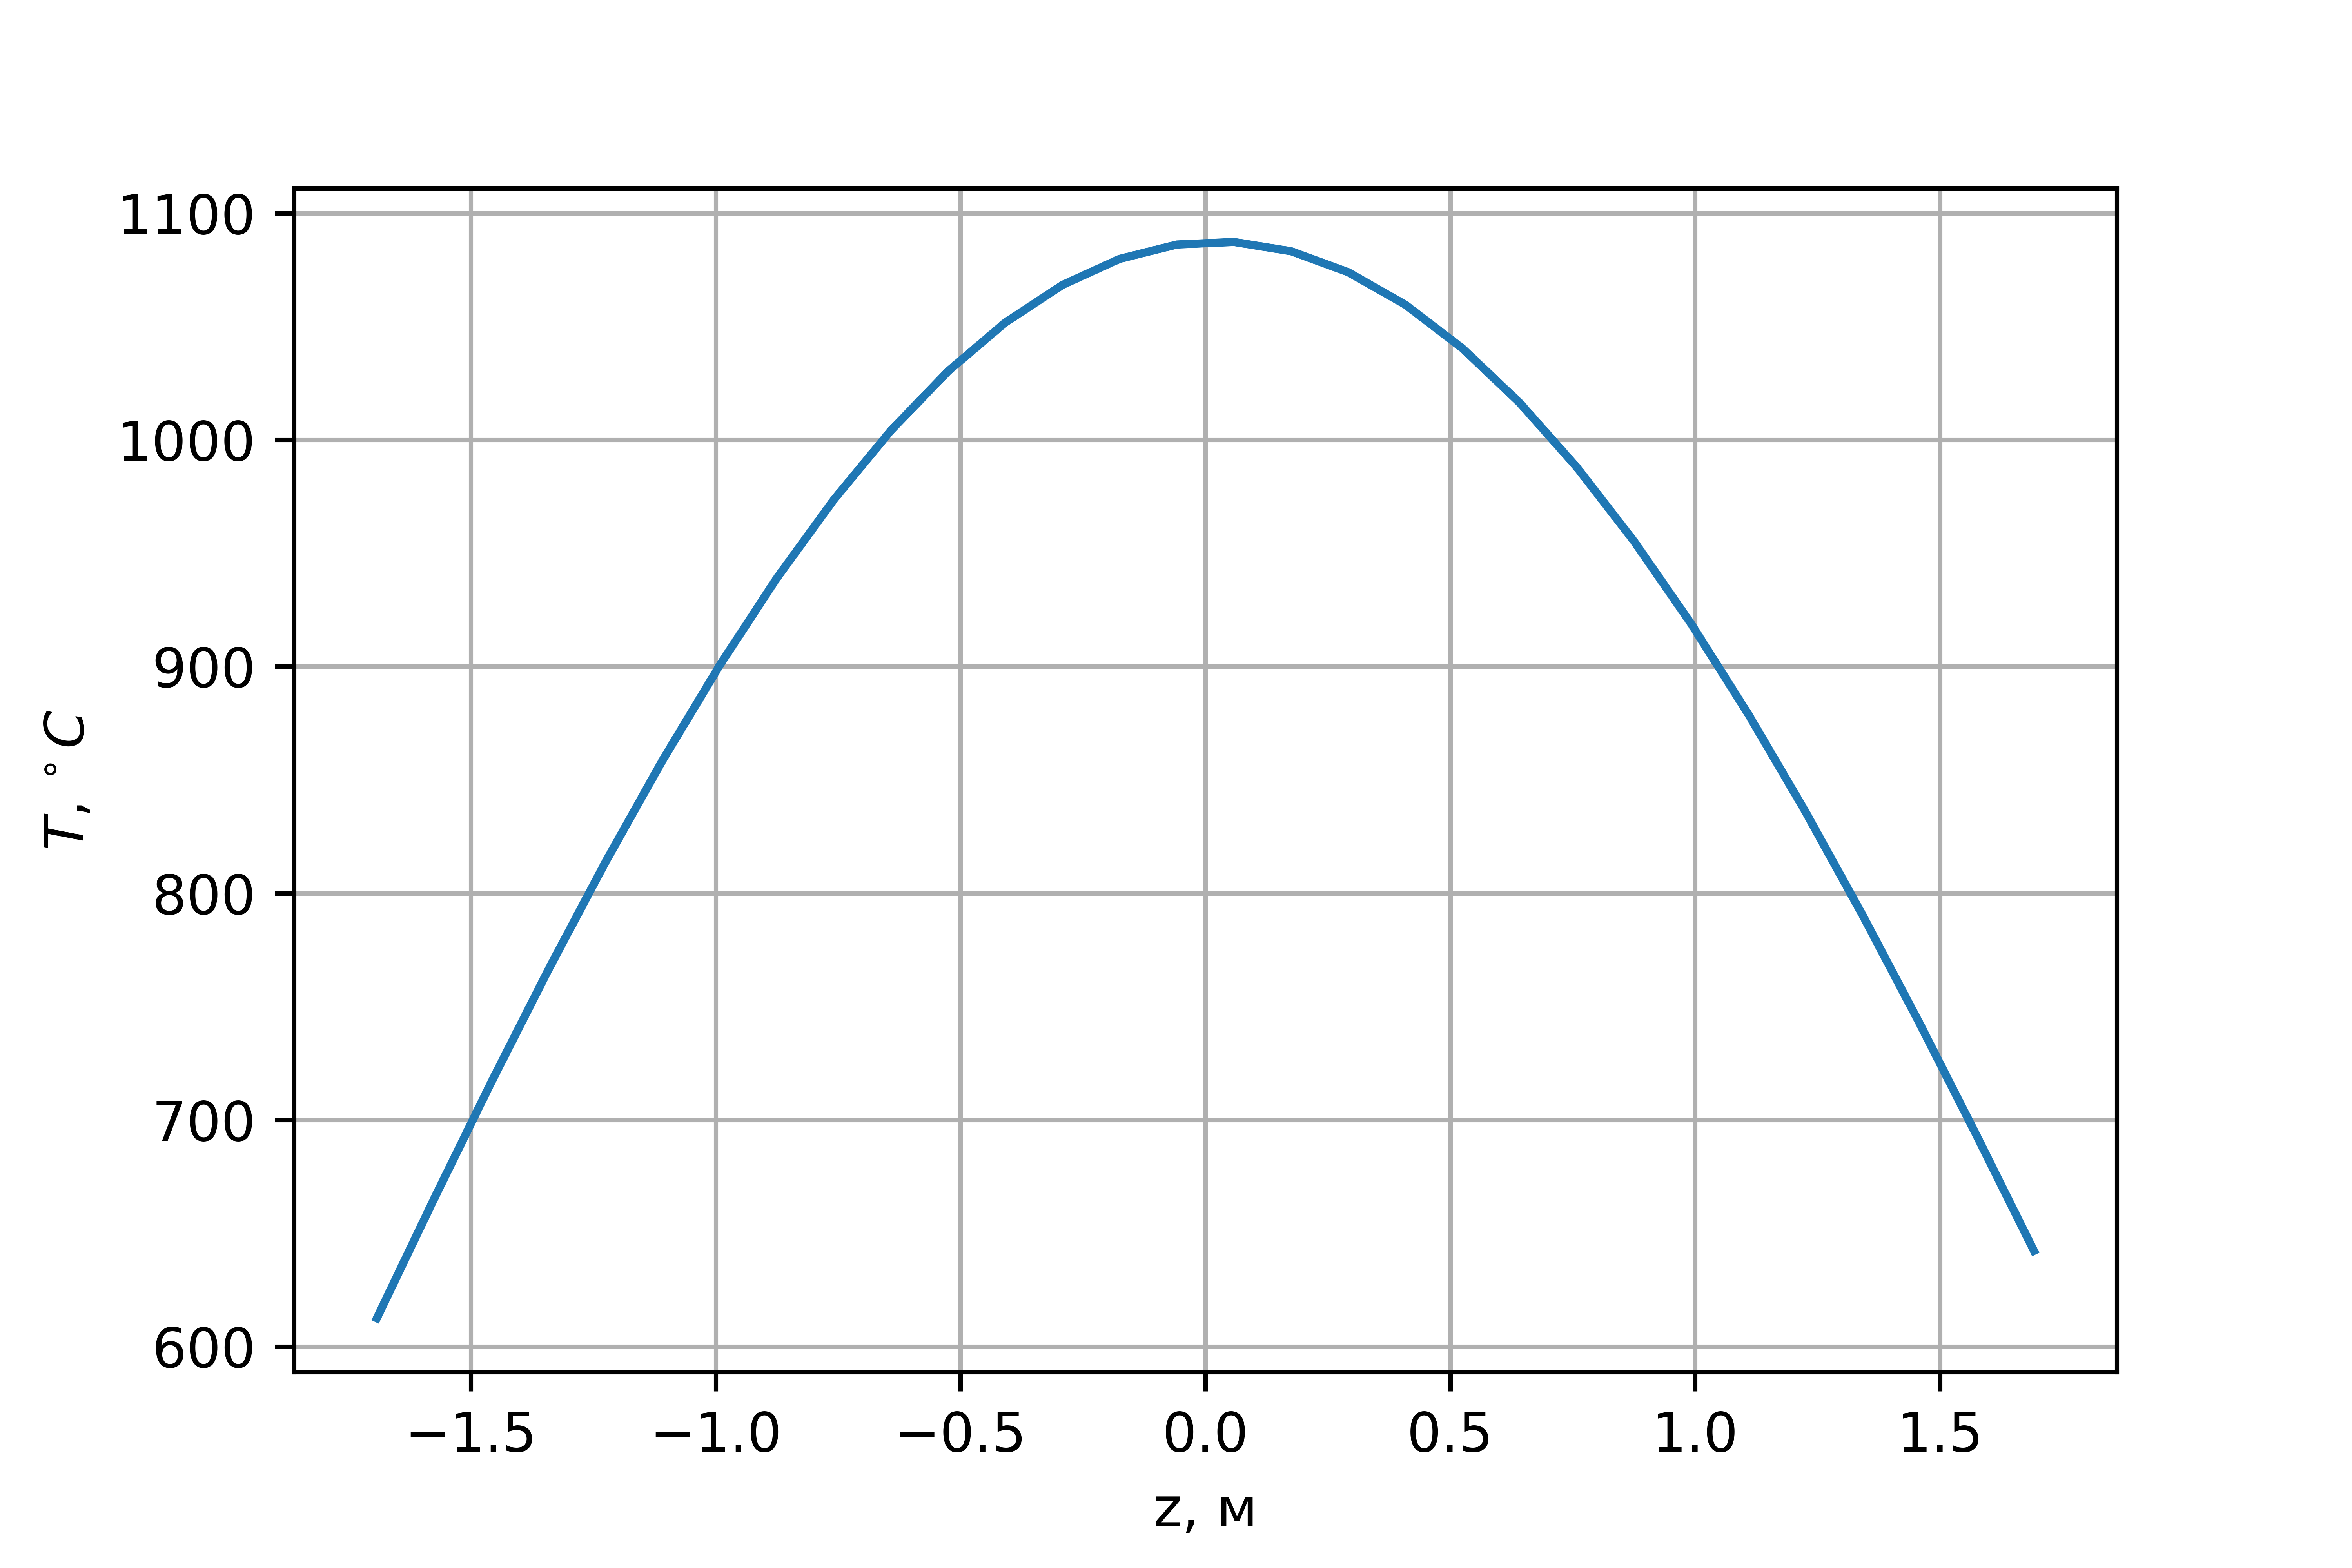
\includegraphics{treton_nominal_t_fuel_max.png}
		\caption{Распределение температуры топлива по высоте АЗ для кассеты с максимальной температурой топлива в центре АЗ}
		\label{pic:treton-t-fuel-nominal-max} % название для ссылок внутри кода
	\end{center}
\end{figure}

\begin{figure}[H]
	\begin{center}
		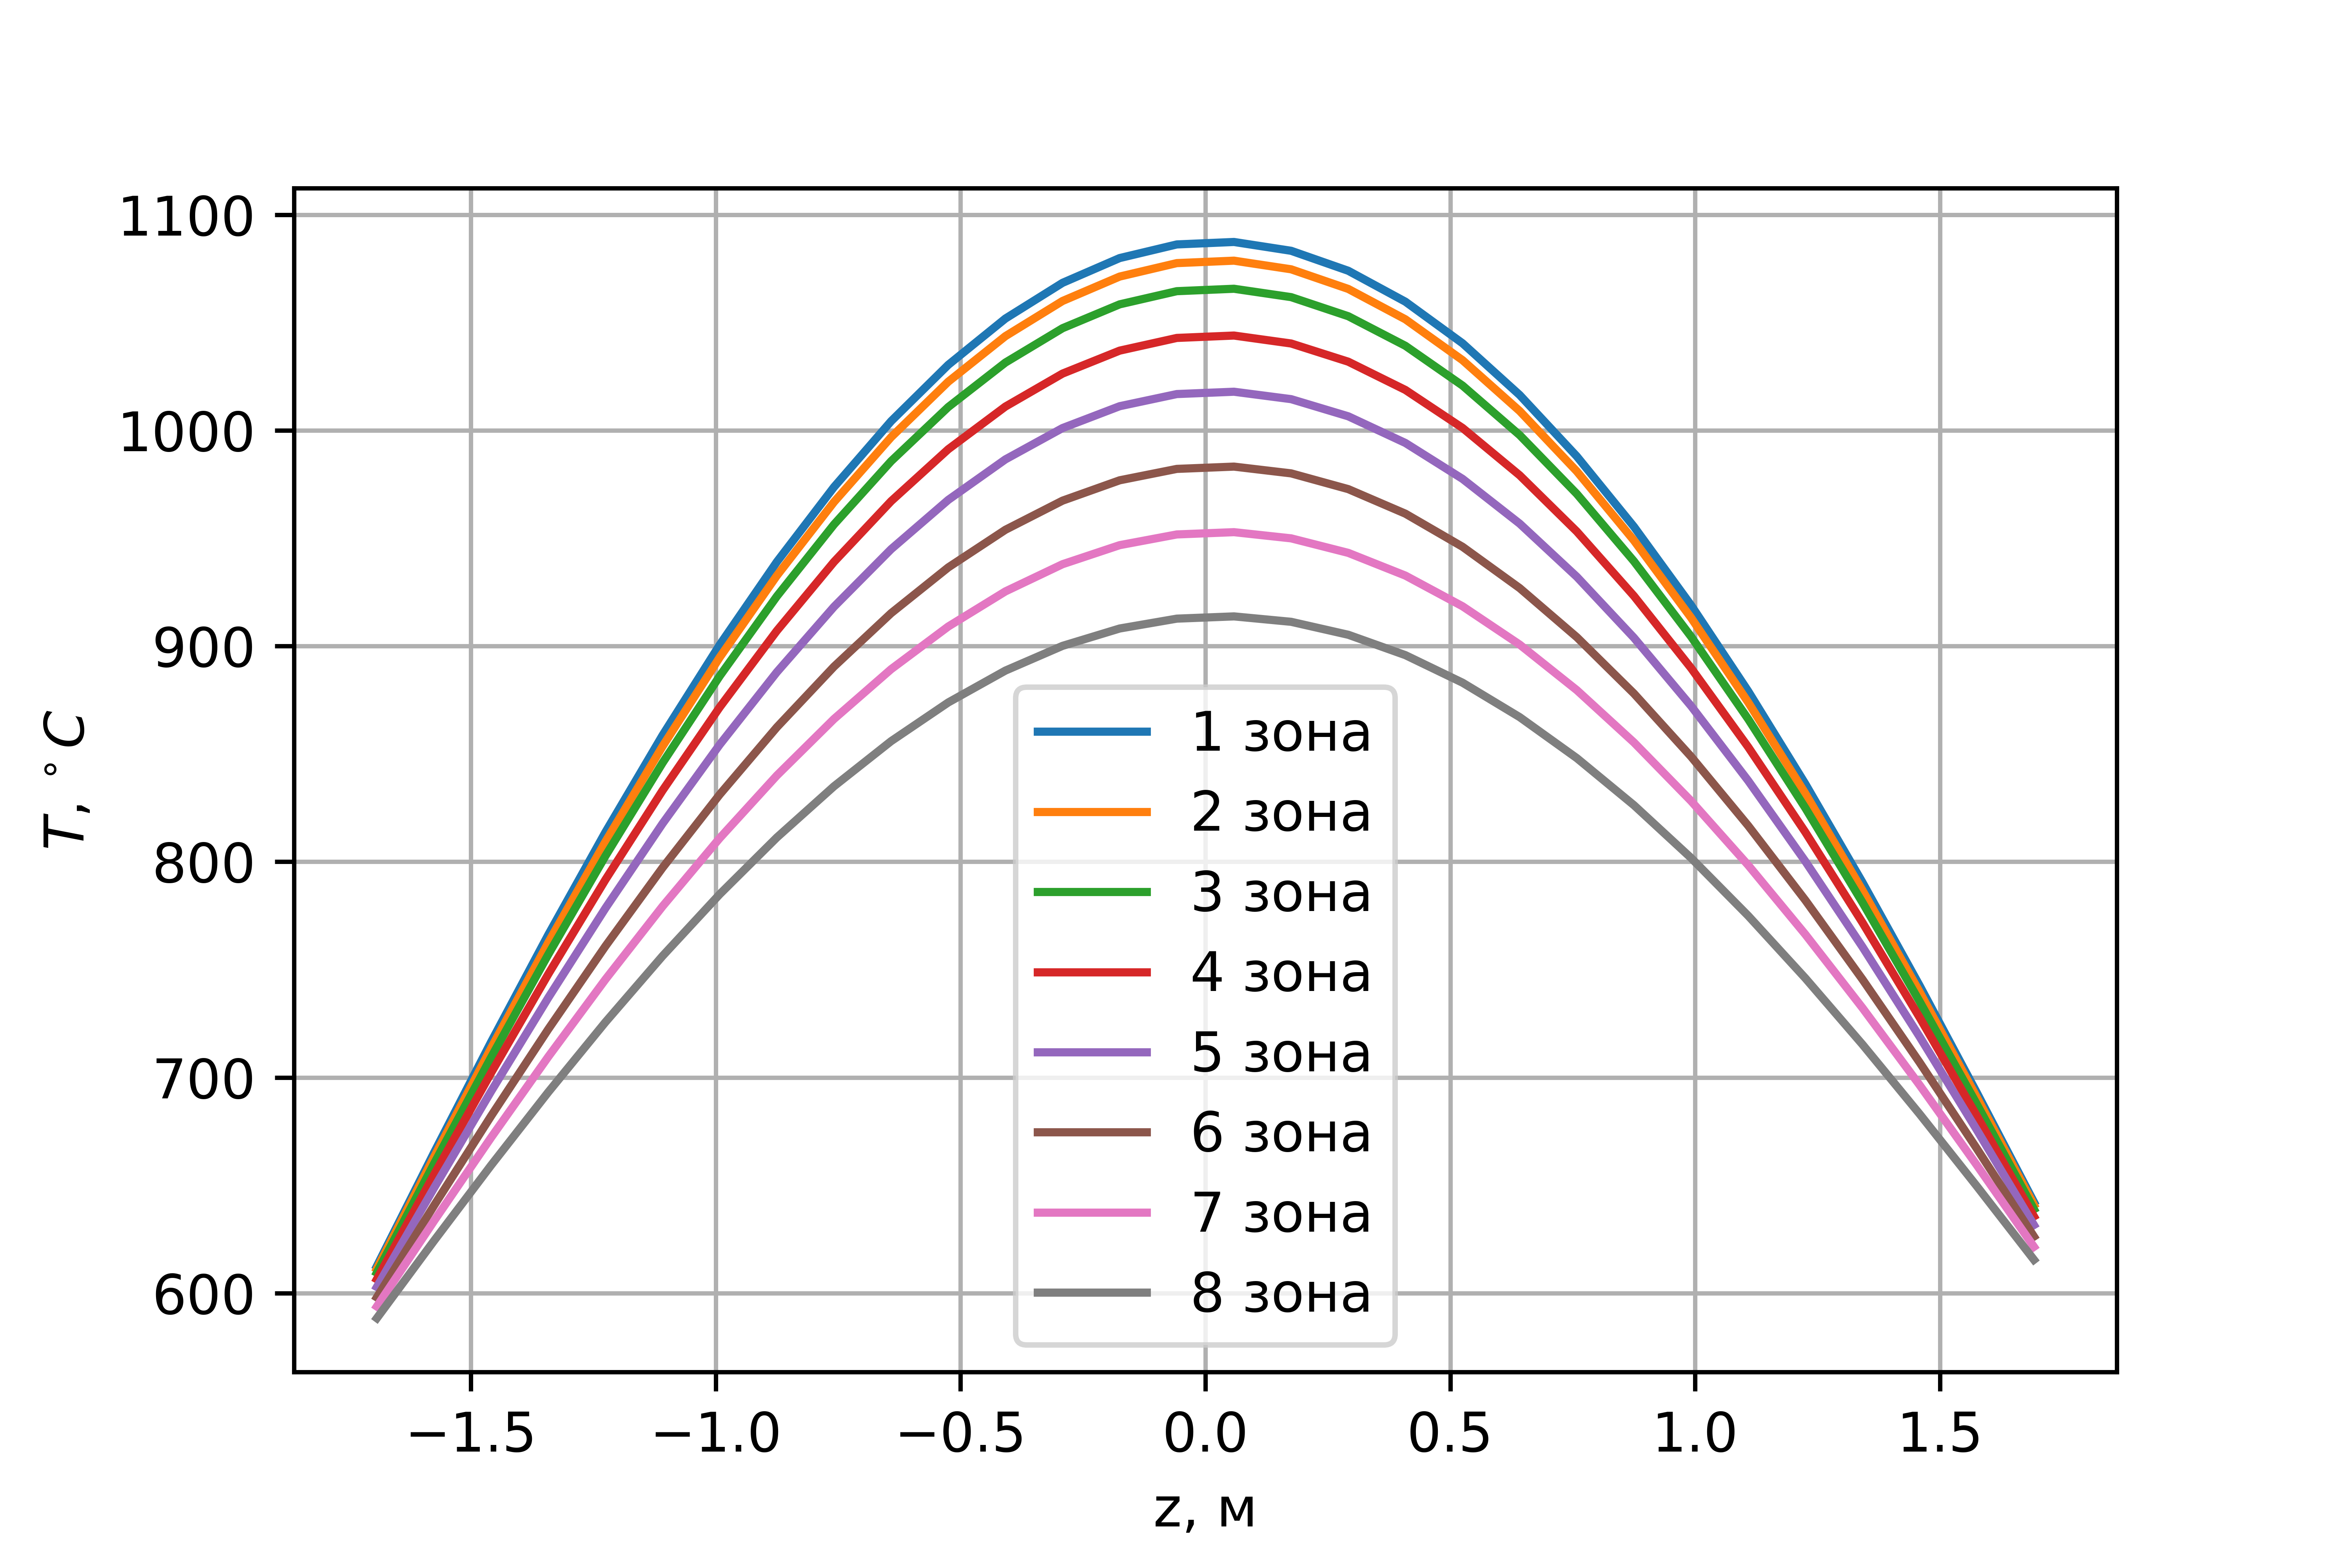
\includegraphics{treton_nominal_t_fuel_by_r.png}
		\caption{Распределение температуры топлива по высоте для всех групп по радиусу АЗ}
		\label{pic:treton-t-fuel-nominal-by-r} % название для ссылок внутри кода
	\end{center}
\end{figure}

Из графиков видно, что максимальная температура топлива
$T_{\text{топ} \text{Ном}}^{\max} = 1087.4 ^\circ C$, что не превышает максимально допустимую при авариях температуру плавления оксида урана $2600 ^\circ C$

Для ячейки с максимальной температурой также были построены зависимости температуры оболочек от высоты активной зоны. Из рис \ref{pic:treton-t-obl-naruj-nominal-max} максимальная температура оболочки составляет $346.46 ^\circ C$, запас до кипеня теплоносителя около стенки составляет $0.04, ^\circ C$, из чего можно сделать вывод что пристеночное кипения не наблюдается

\begin{figure}[H]
	\begin{center}
		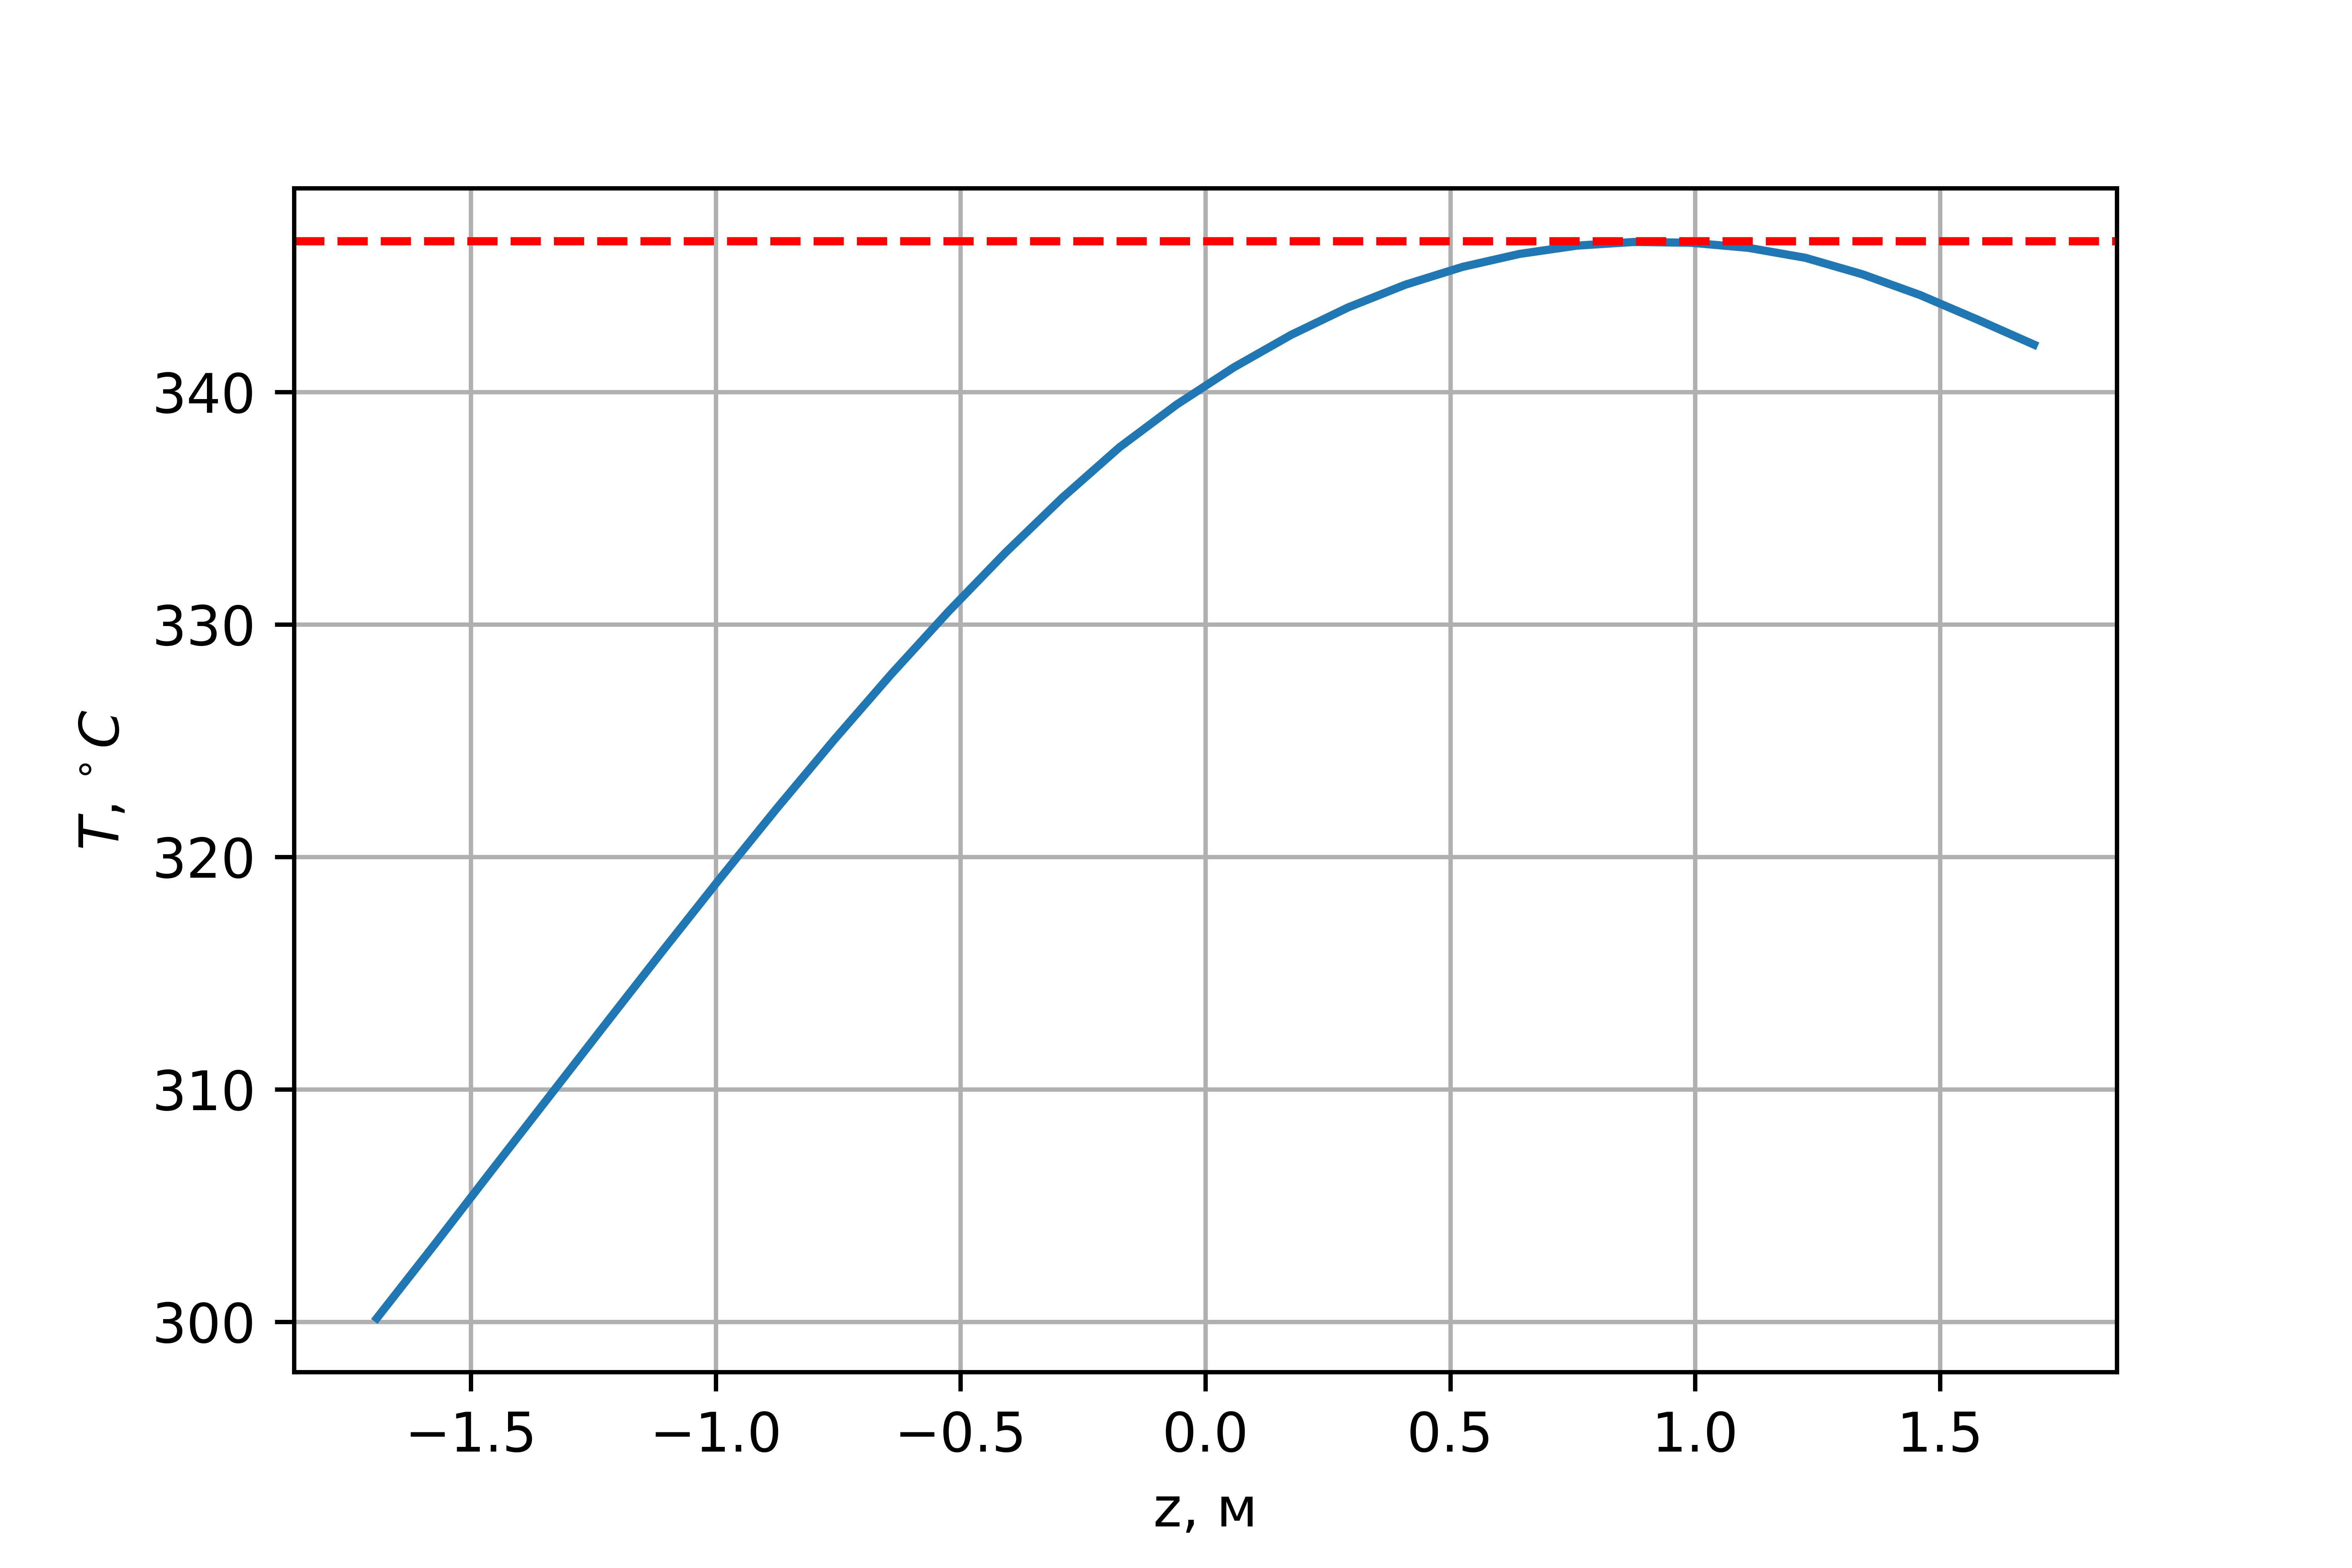
\includegraphics{treton_nominal_obl_naruj_max.png}
		\caption{Распределение температуры внешней оболочки по высоте для кассеты с максимальной температурой на выходе из АЗ}
		\label{pic:treton-t-obl-naruj-nominal-max} % название для ссылок внутри кода
	\end{center}
\end{figure}

На рис \ref{pic:treton-obl-tepl-obsh-nominal} представлен  общий график для распределения температур наружней, внутренней оболочки и теплоносителя

\begin{figure}[H]
	\begin{center}
		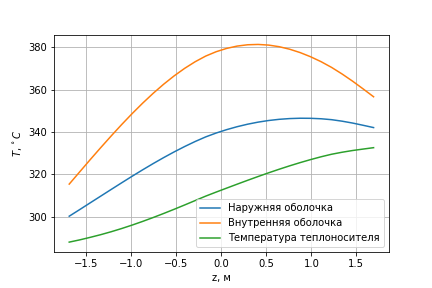
\includegraphics{treton_nominal_obl_tepl_obsh.png}
		\caption{Распределение температур оболочек и теплоносителя по высоте АЗ}
		\label{pic:treton-obl-tepl-obsh-nominal} % название для ссылок внутри кода
	\end{center}
\end{figure}

Для ячейки с максимальной температурой топлива на выходе также было построено распределение давления теплоносителя по высоте активной зоны, которое представлено на рисунке \ref{pic:treton-p-nominal-max}.

\begin{figure}[H]
	\begin{center}
		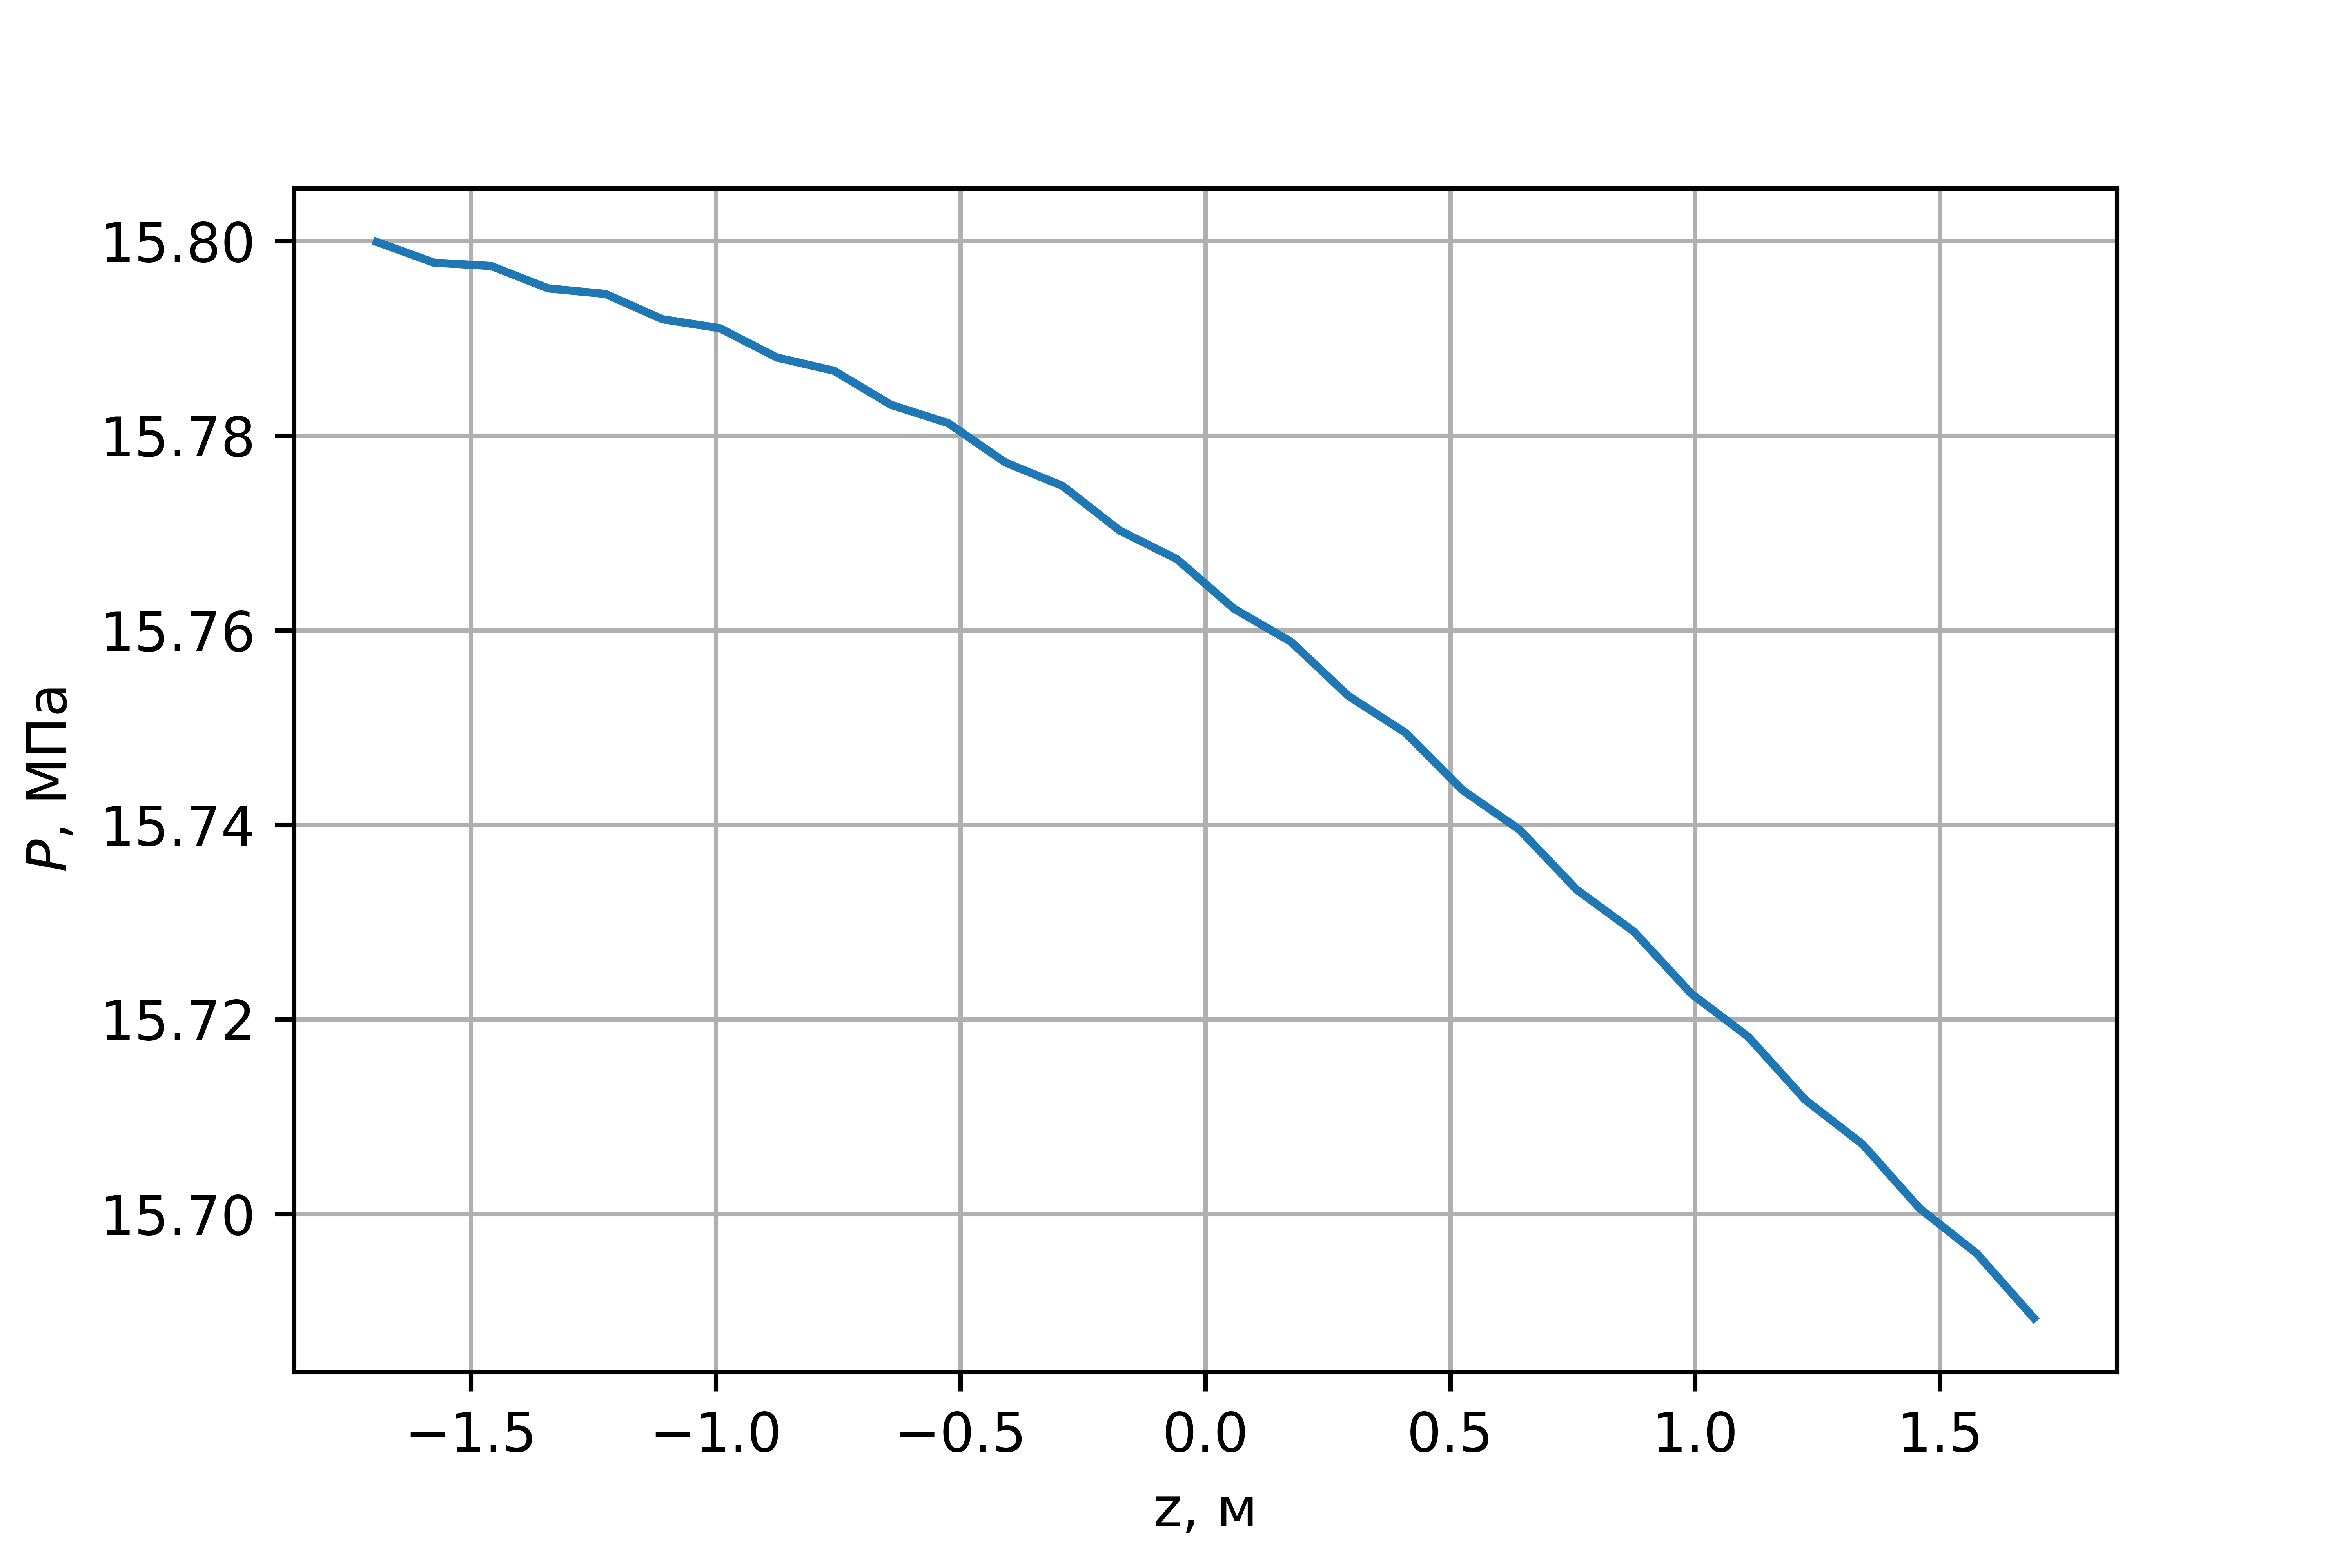
\includegraphics{p_nominal_max.png}
		\caption{Распределение давления в кассете с максимальной температурой на выходе по высоте активной зоны}
		\label{pic:treton-p-nominal-max} % название для ссылок внутри кода
	\end{center}
\end{figure}

Для каждой ТВС были расчитаны подогревы теплоносителя. На \ref{pic:treton-podogrev-nominal} представлено распределение подогрева по каждой кассете ТВС, на \ref{pic:treton-podogrev-nominal-by-r} усредненное распределение по радиальным группам ТВС в соответствии с разбиением представленным на картограмме \ref{pic:treton-kartogramma}.


\begin{figure}[H]
	\begin{center}
		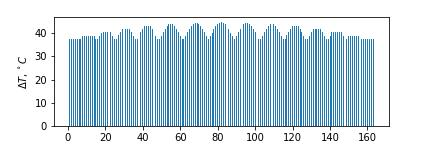
\includegraphics{podogrev_nominal.jpg}
		\caption{Распределение подогревов ТВС}
		\label{pic:treton-podogrev-nominal} % название для ссылок внутри кода
	\end{center}
\end{figure}

\begin{figure}[H]
	\begin{center}
		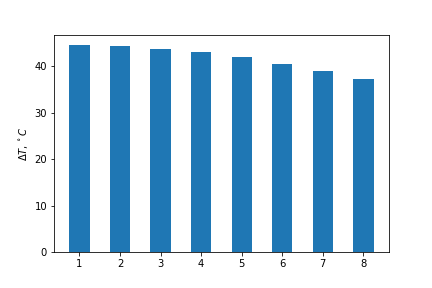
\includegraphics{podogrev_nominal_by_r.png}
		\caption{Распределение подогревов ТВС усредненное по группам}
		\label{pic:treton-podogrev-nominal-by-r} % название для ссылок внутри кода
	\end{center}
\end{figure}

% TODO: график расхода

\subsection{Расчет теплогидравлических характеристик при работе на повышенной мощности}
Ввиду наличия успешных практик перевода работы реакторов ВВЭР-1000 на повышенную мощность для расматриваемой реакторной установки были выполнены соответствующие теплогидравлические расчеты програмным комплексом «ТРЕТОН. 

Было проведено исследование температур РУ при разных мощностях с целью подбора оптимальной мощности. Оптимальной принималась такая мощность выше номинальной, при которой вклад возникающего пристеночного кипения незначителен в приближении расчетной модели. Экспериментальным путем было выяснено, что вклад пристеночного кипения незначителен, если если наблюдается превышение температуры кипения теплоносителя не более чем на 3 $^\circ C$. Результаты исследования температур в сравнении с номинальным режимом представлены в таблице \ref{tabular:t_max_nominal_compare}. Были рассмотрены режимы работы реактора при повышении мощности на 5\%, 10\% и 15\% и номинальных значений температур на входе в активную зону. Для моделирования таких режимов работы полученная зависимость тепловыделения от радиуса и высоты для номинального режима \ref{equation:Qzr} была промасштабирована коэфициентом $\gamma = \overline{1.05, 1.1, 1.15}$


\begin{equation}
	Q_{ \gamma N_{\text{ном}}}(z,r) 
	= \gamma \cdot Q(z,r) 
	= K_r(r) K_z \cos \left( 
		\frac{\pi z}{H_{\text{эфф}}} 
	  \right) 
	  \frac{\gamma \cdot Q_{\text{теп}}}{N_{\text{ТВС}} 30}
\end{equation}

Для сравнения возникающего пристеночного кипения на рисунке \ref{pic:treton-obl-naruj-max-compare} была построена зависимость температуры внешней оболочки от высоты для всех рассматриваемых мощностей. Из \ref{pic:treton-obl-naruj-max-compare} для мощностей 10 и 15\% выше номинальной наблюдается плато в районе максимума температур в следствие существенного влияния пристеночного кипения. Исходя из этого повышение мощности на 5 \% оптимально для дальнейшего анализа ввиду разности температуры оболочки и температуры кипения теплоносителя кипения не более чем на 3 $^\circ C$. 
Для выбранной оптимальной повышенной мощности были построены распределения соответствующих температур по высоте, которые представлены на рисунках \ref{pic:treton-t-fuel-povish-compare}, \ref{pic:treton-t-tepl-povish-compare}, \ref{pic:treton-povish-obl-naruj-max}. 

% TODO: таблица
% сразу графички в сравнении с температурами кипения

\begin{table}[H]
    \caption{Максимальные температуры теплоносителя, топлива и оболочки твэлов при работе РУ на номинальной и повышенной мощности}
    \begin{center}
        \begin{tabular}{|l|c|c|c|c|}
        \toprule
        Тепловая мощность, МВт & 2903 & 3048.8 & 3194 & 3339.2 \\
        \midrule
        \hline
        Максимальная температура теплоносителя, $\circ C$ & 332.5 & 333.9 & 334.9 & 336.3  \\ 
        \hline
        Запас до кипения теплоносителя, $\circ C$ & 13.9 & 12.6 & 11.6 &  10.17 \\
        \hline
        Максимальная температура топлива, $\circ C$ & 1452 & 1465 & 1501.8 & 1538.4  \\
        \hline
        Максимальная температура внешней оболочки & 346.46 & 347.9 & 349  & 349.4 \\
        \hline
        Максимальная температура внутренней оболочки & 381.3 & 383 & 385.9 & 389.7 \\
        \hline
        Разность температуры кипения теплоносителя\\ и температуры внешней оболочки & 0.04 & -1.4 & -2.5 & -2.9 \\
        \bottomrule
        \end{tabular}
		\label{tabular:t_max_nominal_compare}
    \end{center}
\end{table}

\begin{figure}[H]
	\begin{center}
		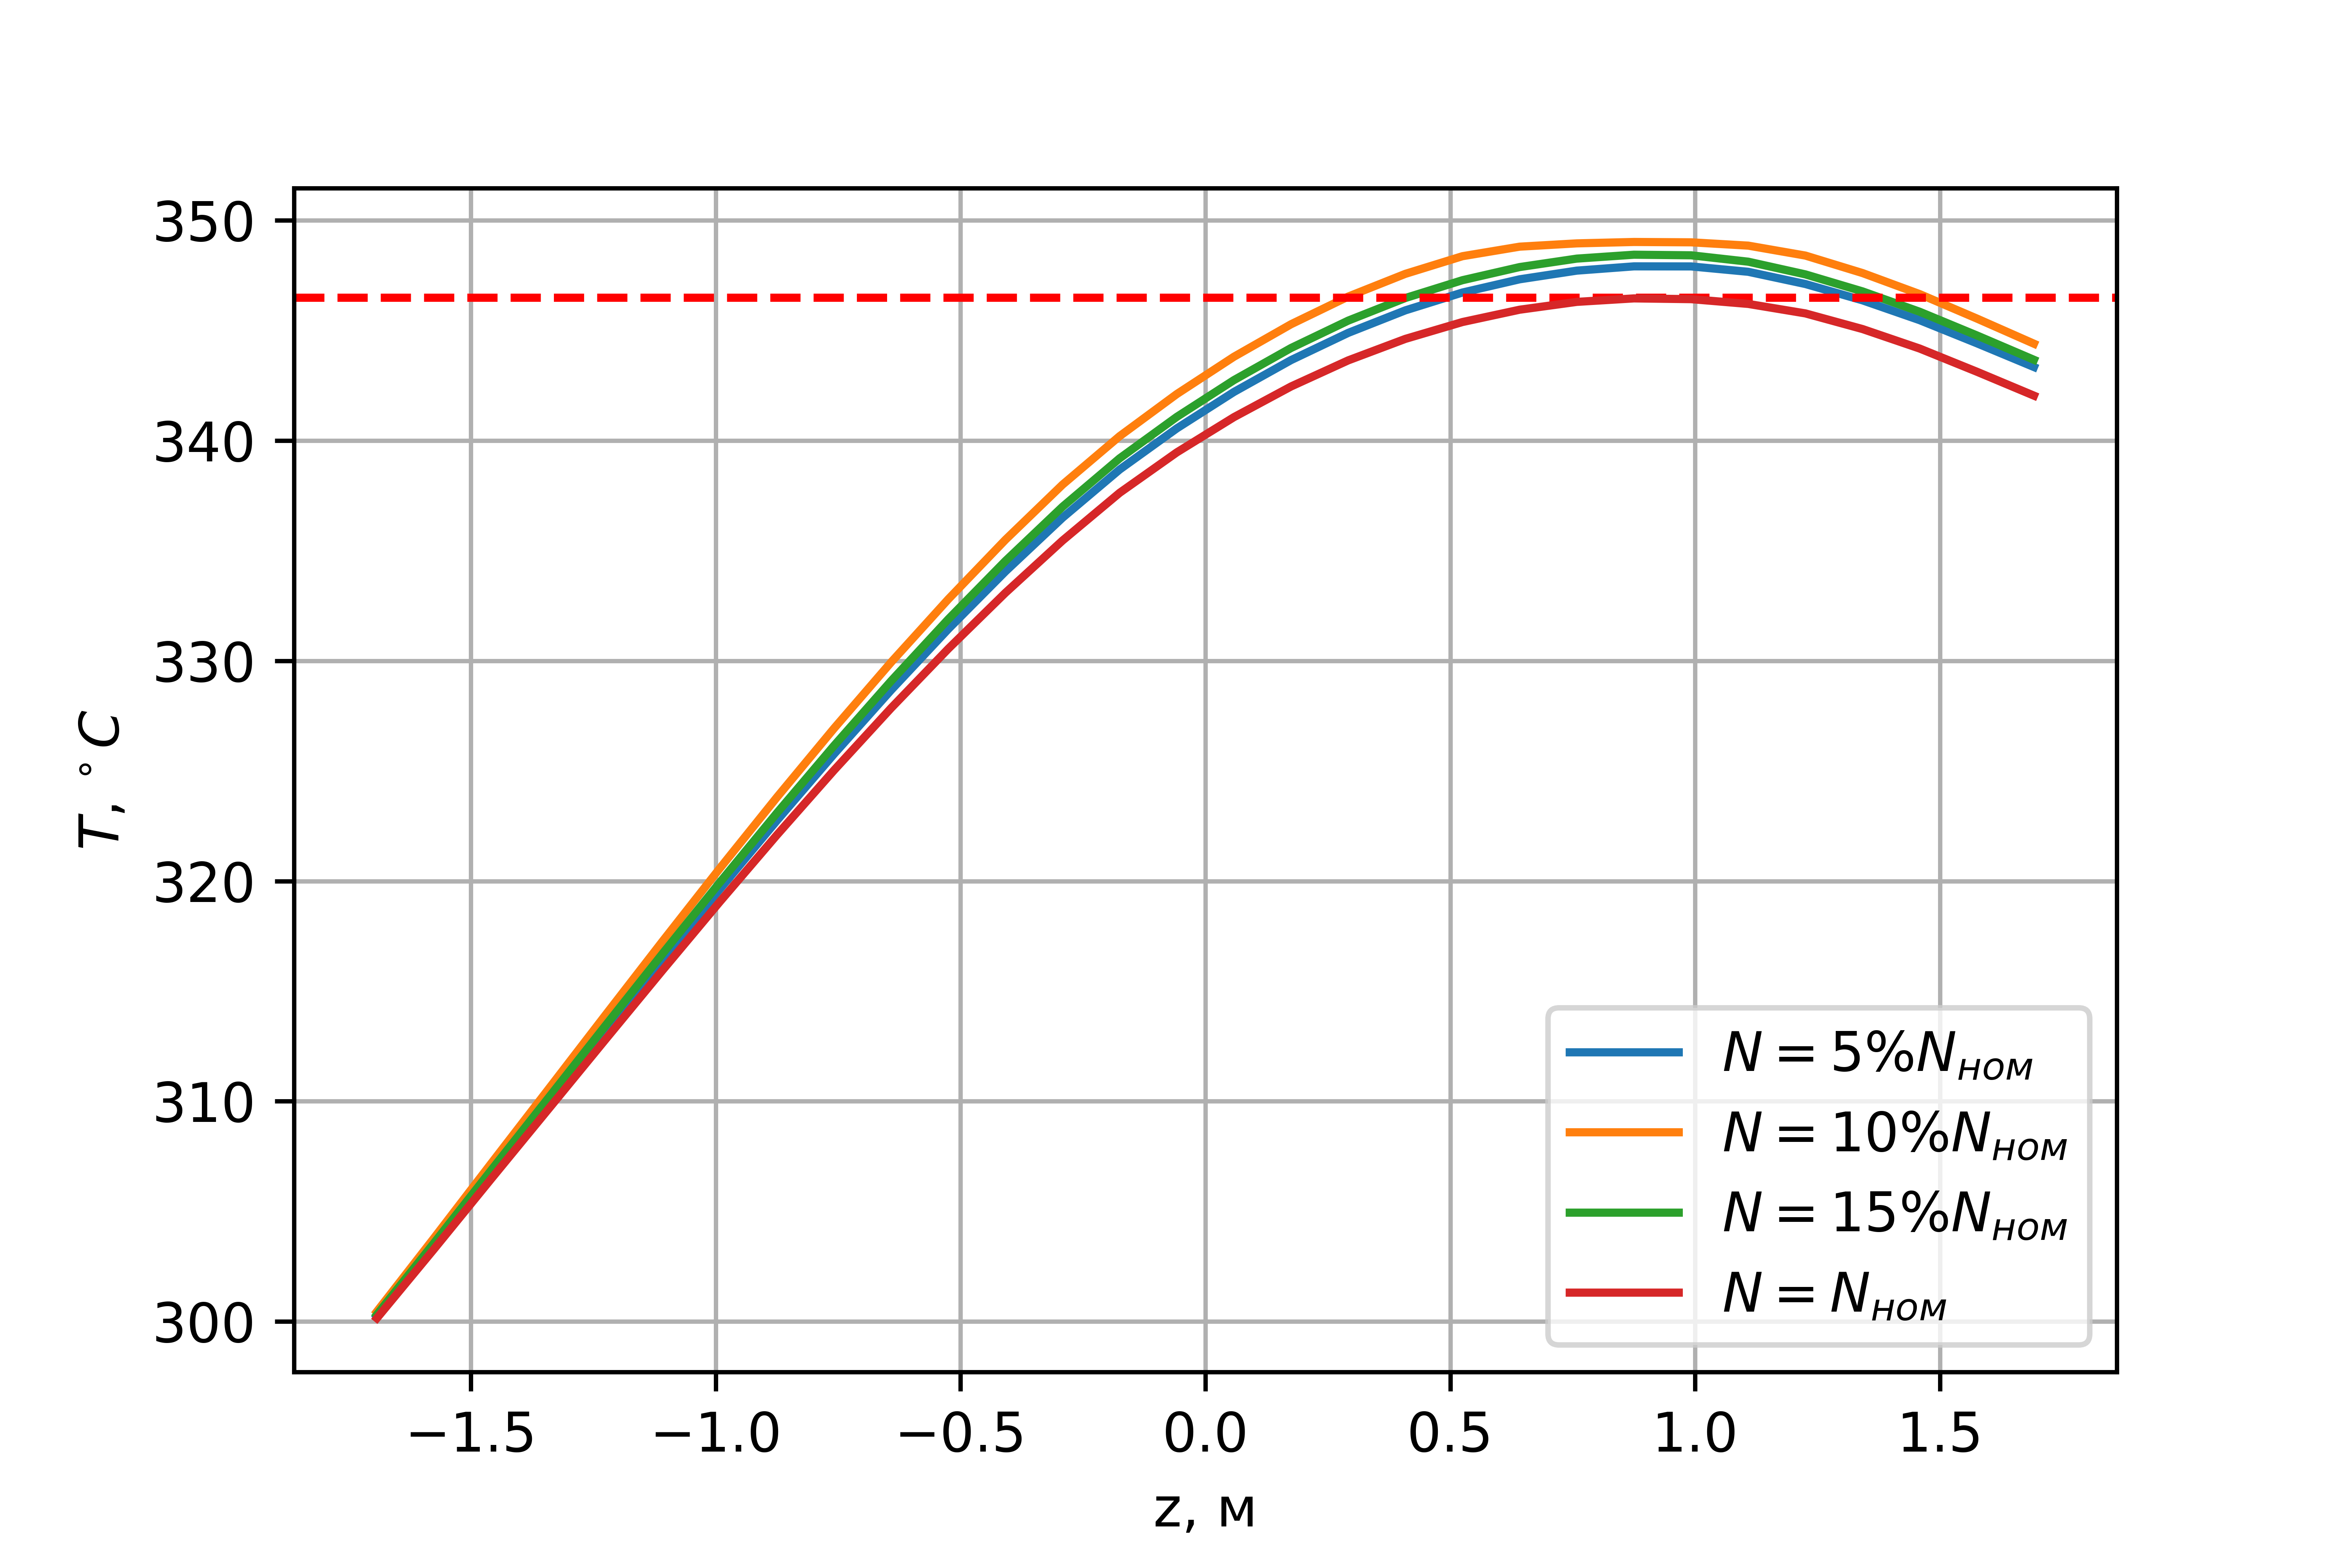
\includegraphics{treton_obl_naruj_max_compare.png}
		\caption{Распределение температуры внешней оболчоки по высоте активной зоны для работы реактора на повышенных мощностях }
		\label{pic:treton-obl-naruj-max-compare} % название для ссылок внутри кода
	\end{center}
\end{figure}

\begin{figure}[H]
	\begin{center}
		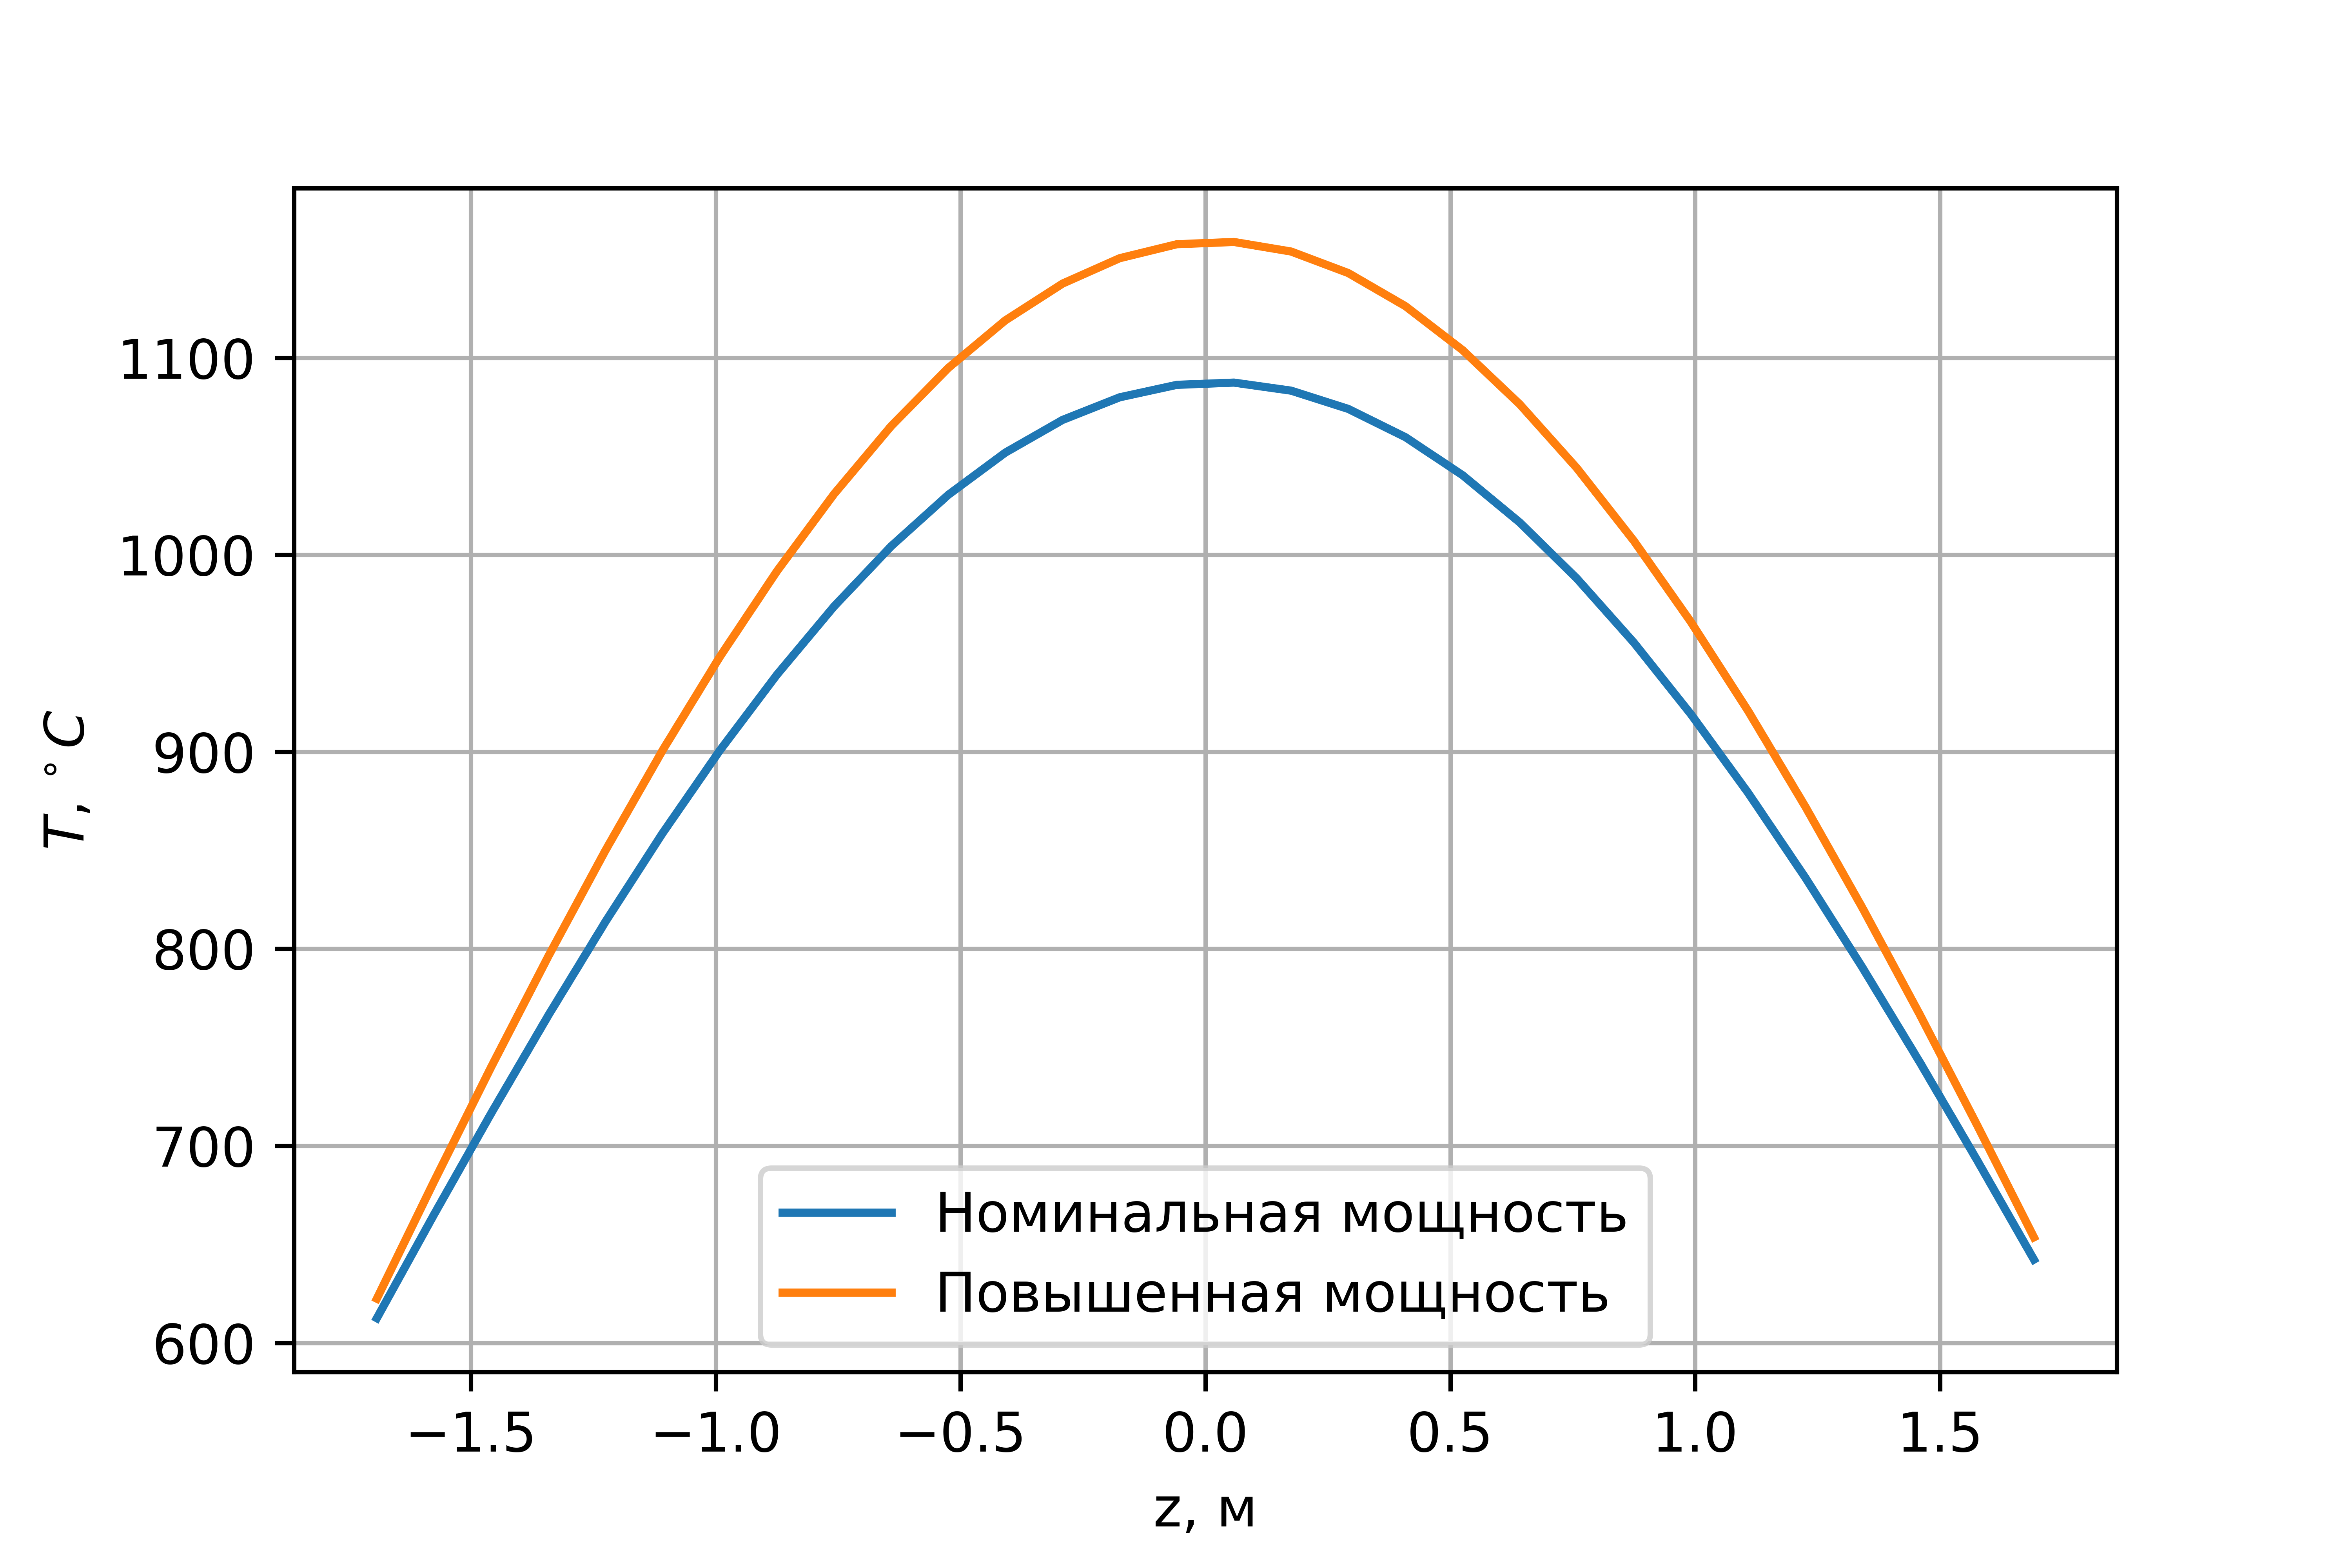
\includegraphics{treton_t_fuel_povish_compare.png}
		\caption{Распределение температуры топлива по высоте АЗ}
		\label{pic:treton-t-fuel-povish-compare} % название для ссылок внутри кода
	\end{center}
\end{figure}

\begin{figure}[H]
	\begin{center}
		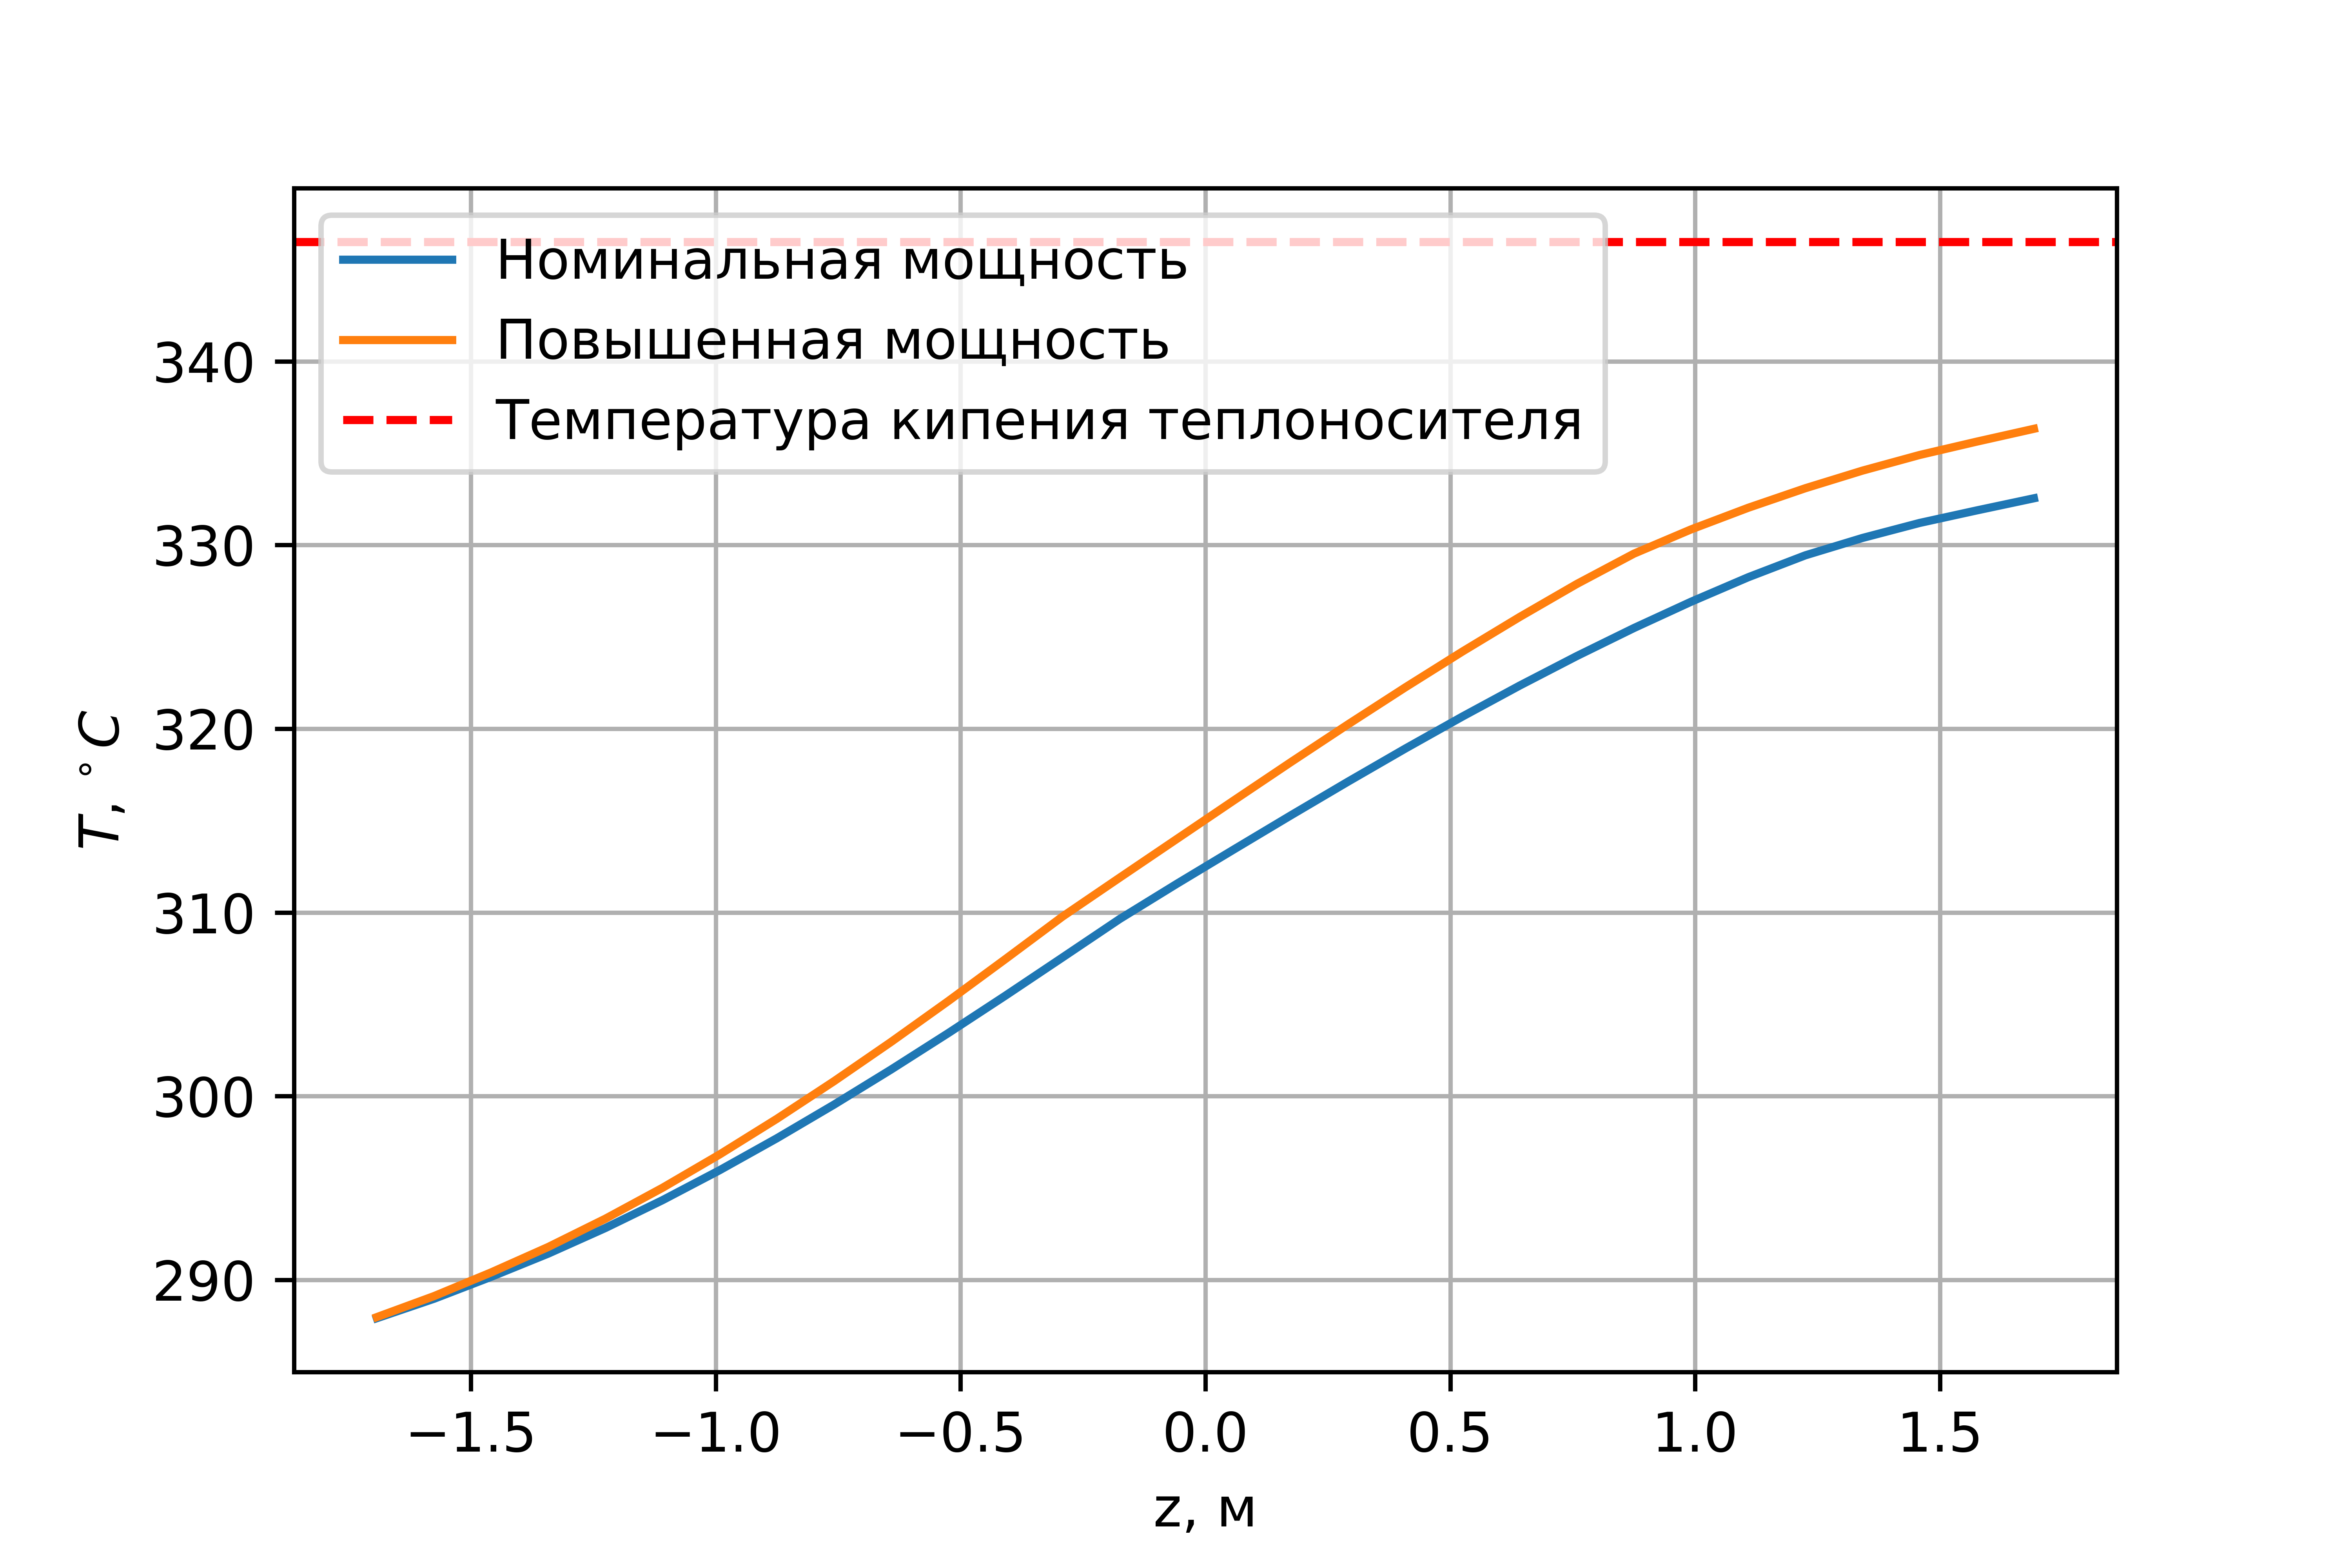
\includegraphics{treton_t_tepl_povish_compare.png}
		\caption{Распределение температуры теплоносителя по высоте АЗ}
		\label{pic:treton-t-tepl-povish-compare} % название для ссылок внутри кода
	\end{center}
\end{figure}

\begin{figure}[H]
	\begin{center}
		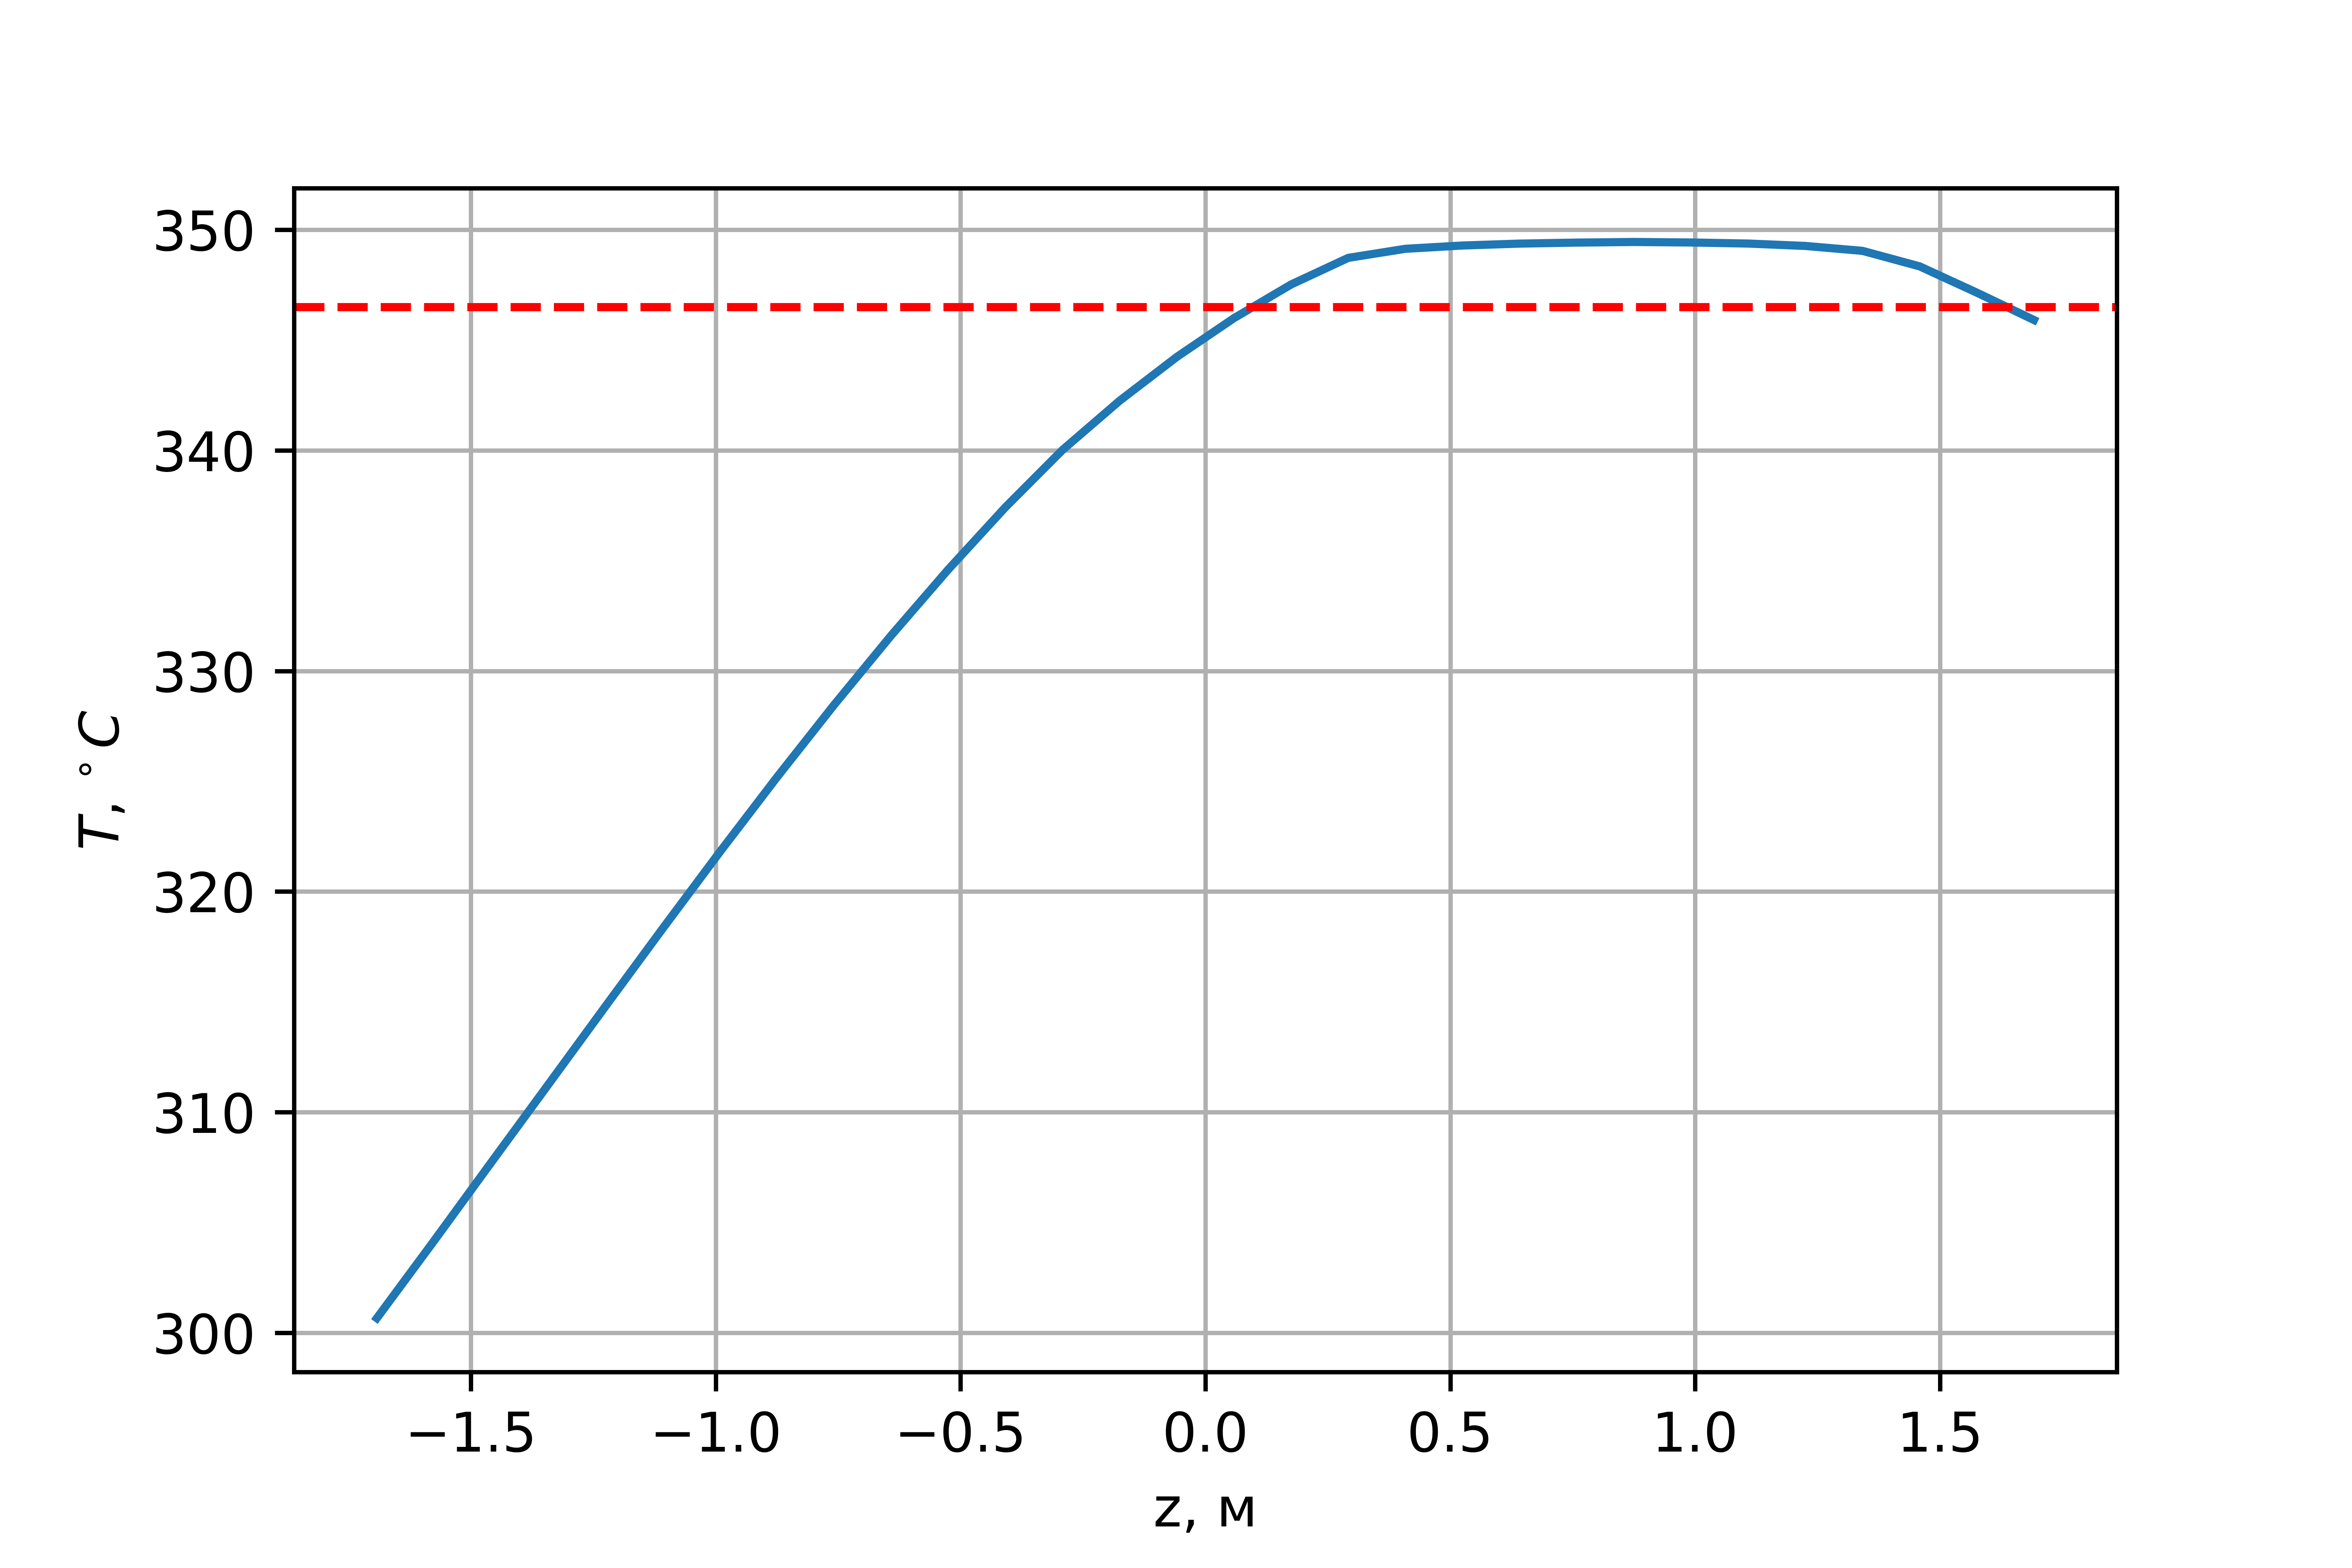
\includegraphics{treton_povish_obl_naruj_max.png}
		\caption{Распределение температуры наруженй оболочки твэлов по высоте для кассеты с максимальной температурой теплоносителя}
		\label{pic:treton-povish-obl-naruj-max} % название для ссылок внутри кода
	\end{center}
\end{figure}

из \ref{tabular:t_max_nominal_compare} видно, что при повышении мощности на 5\% наблюдается превышение максимальной температуры теплоносителя на 1.65 $^\circ C$, что по прежнему не превышает температуру насыщения. Для кассеты с максимальной температурой теплоносителя наблюдается пристеночное кипение вблизи оболочек твэлов, однако температура оболочки превысила температуру кипения теплоносителя на 1.9 $^\circ C$, что говорит нам о его незначительном вкладе в рамках расчетной модели.
Для топлива превышение температуры составило 25.6 $^\circ C$, однако превышения критических для топлва температур не наблюдается. Общий график температур для работы реактора на повышенном уровне мощности представлен на рисунке \ref{pic:treton-povish-obl-tepl-obsh}

\begin{figure}[H]
	\begin{center}
		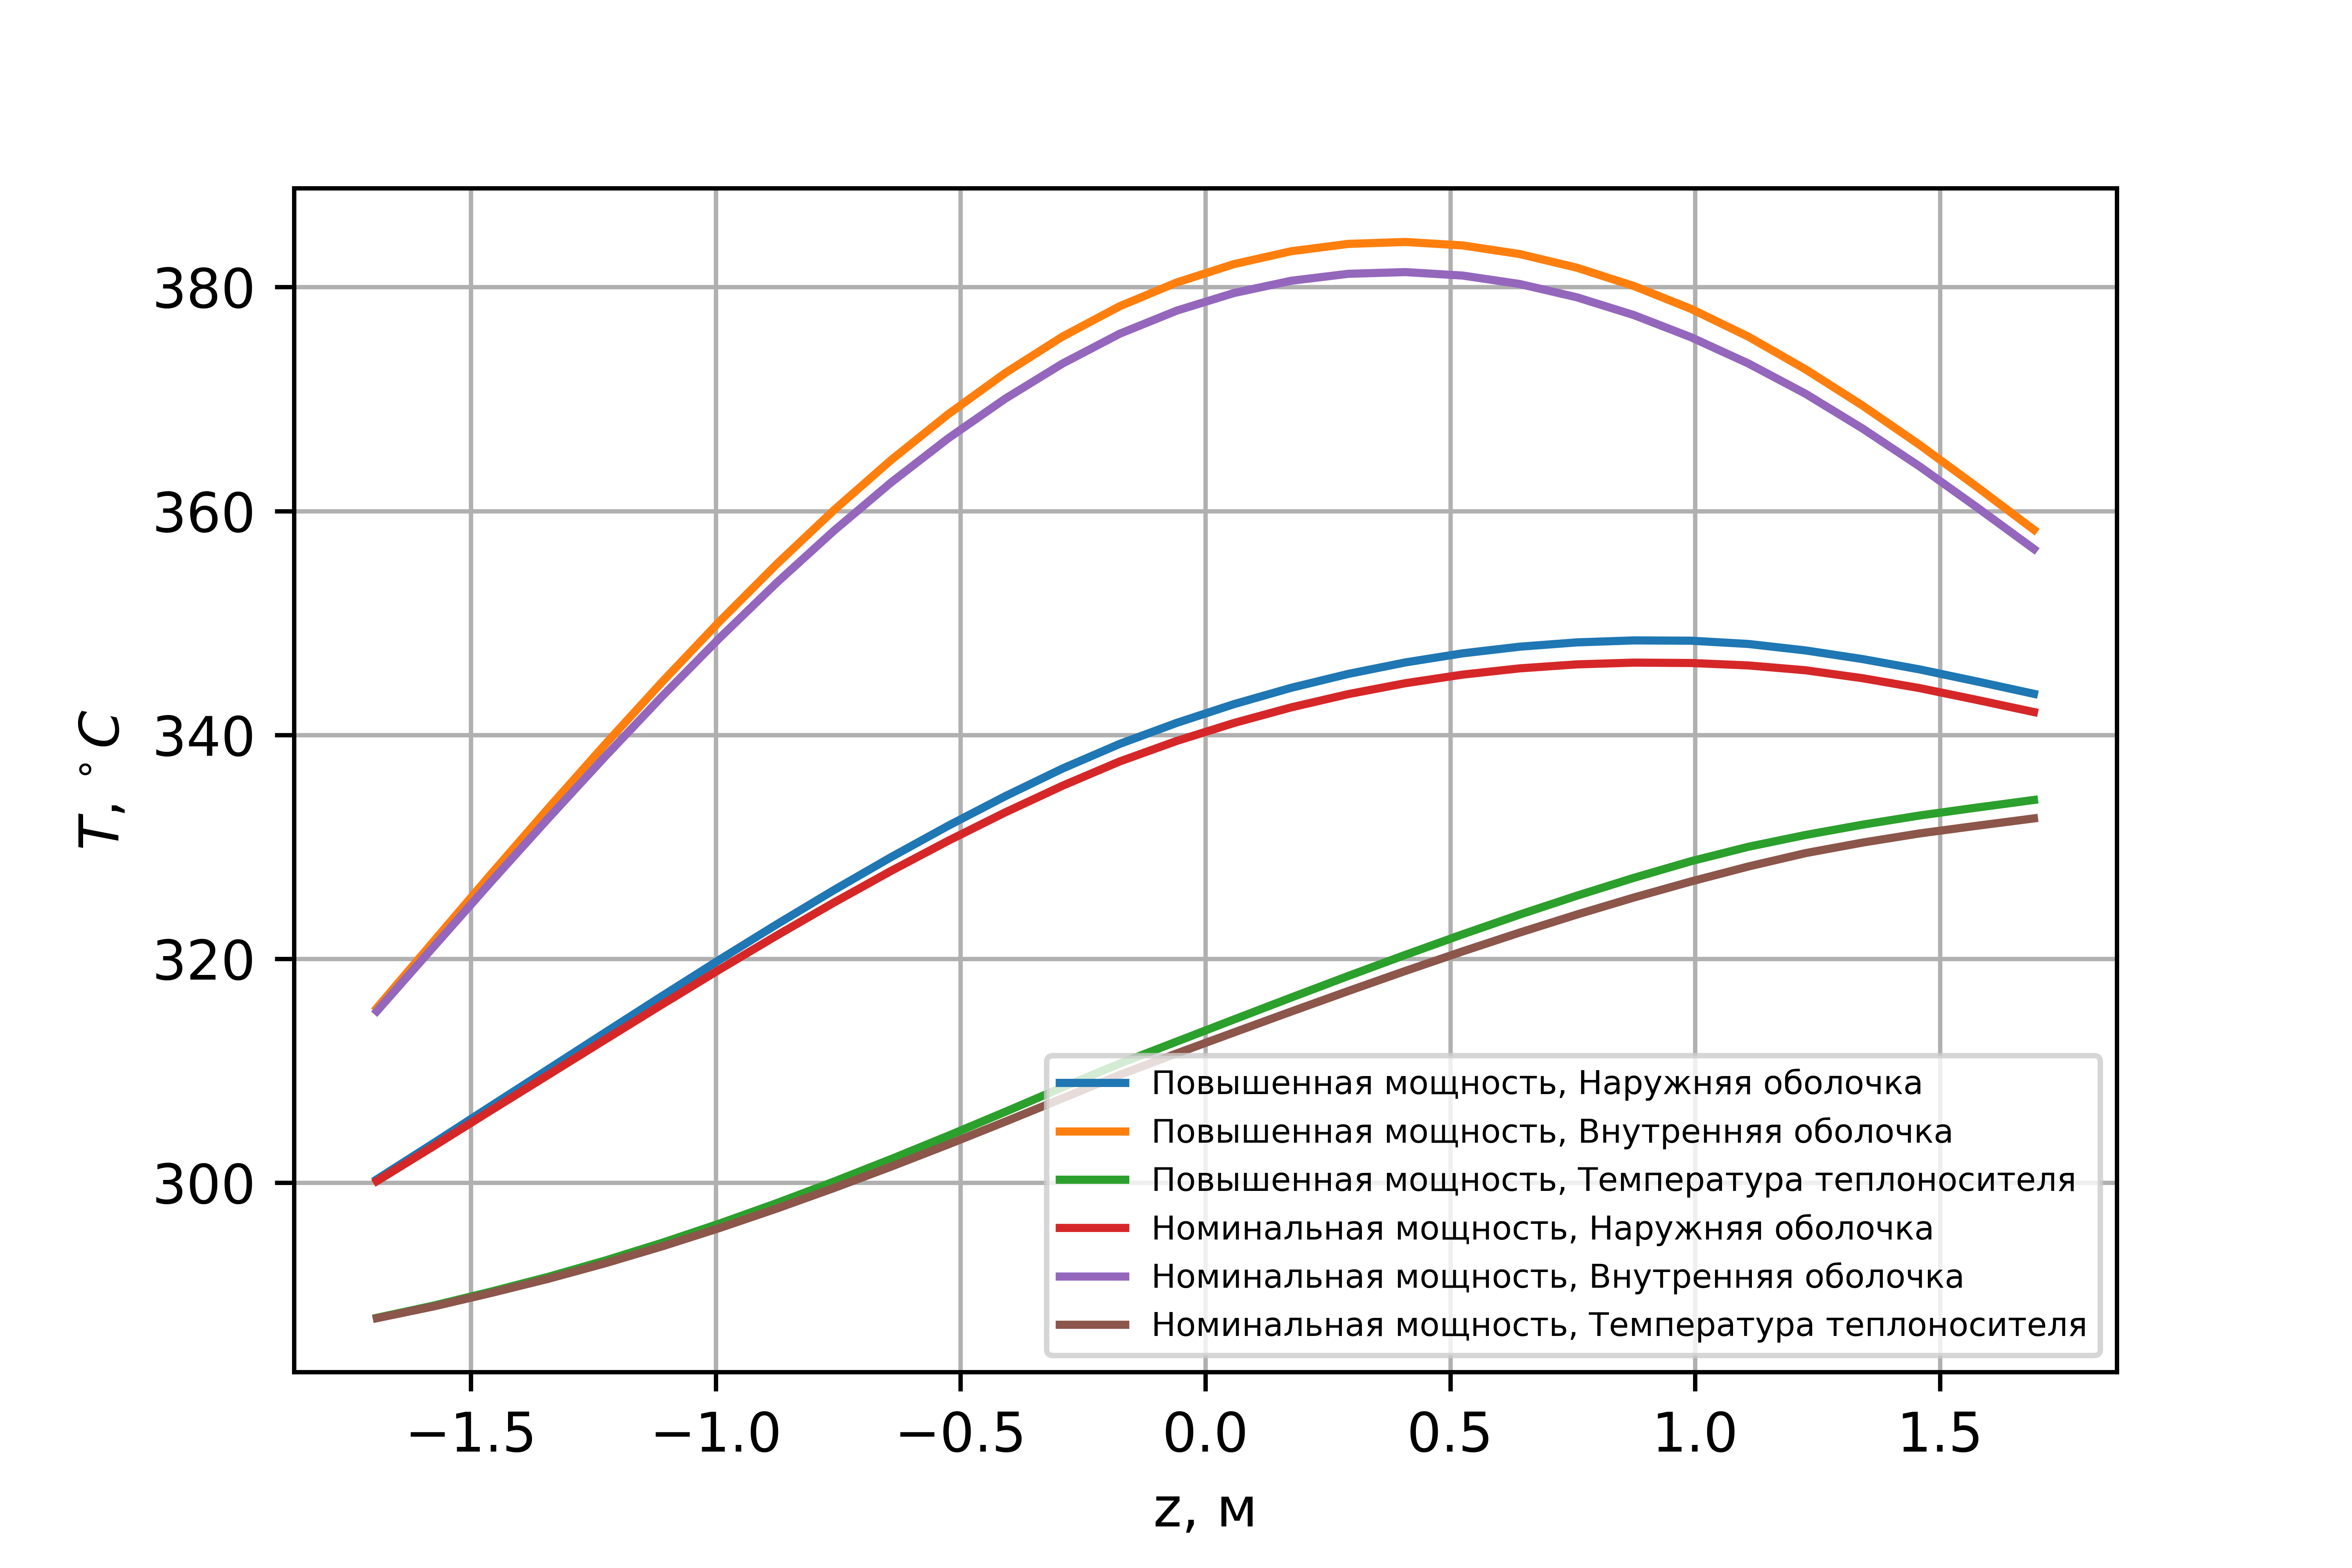
\includegraphics{treton_povish_obl_tepl_obsh.png}
		\caption{Распределение температур по высоте АЗ}
		\label{pic:treton-povish-obl-tepl-obsh} % название для ссылок внутри кода
	\end{center}
\end{figure}


На рисунке \ref{pic:p-povish-max} представлена зависимость давления в кассете с максимальной температурой от высоты. Для давления наблюдается понижение в центре ТВС на 5 КПа по сравнению с номинальным режимом. 


\begin{figure}[H]
	\begin{center}
		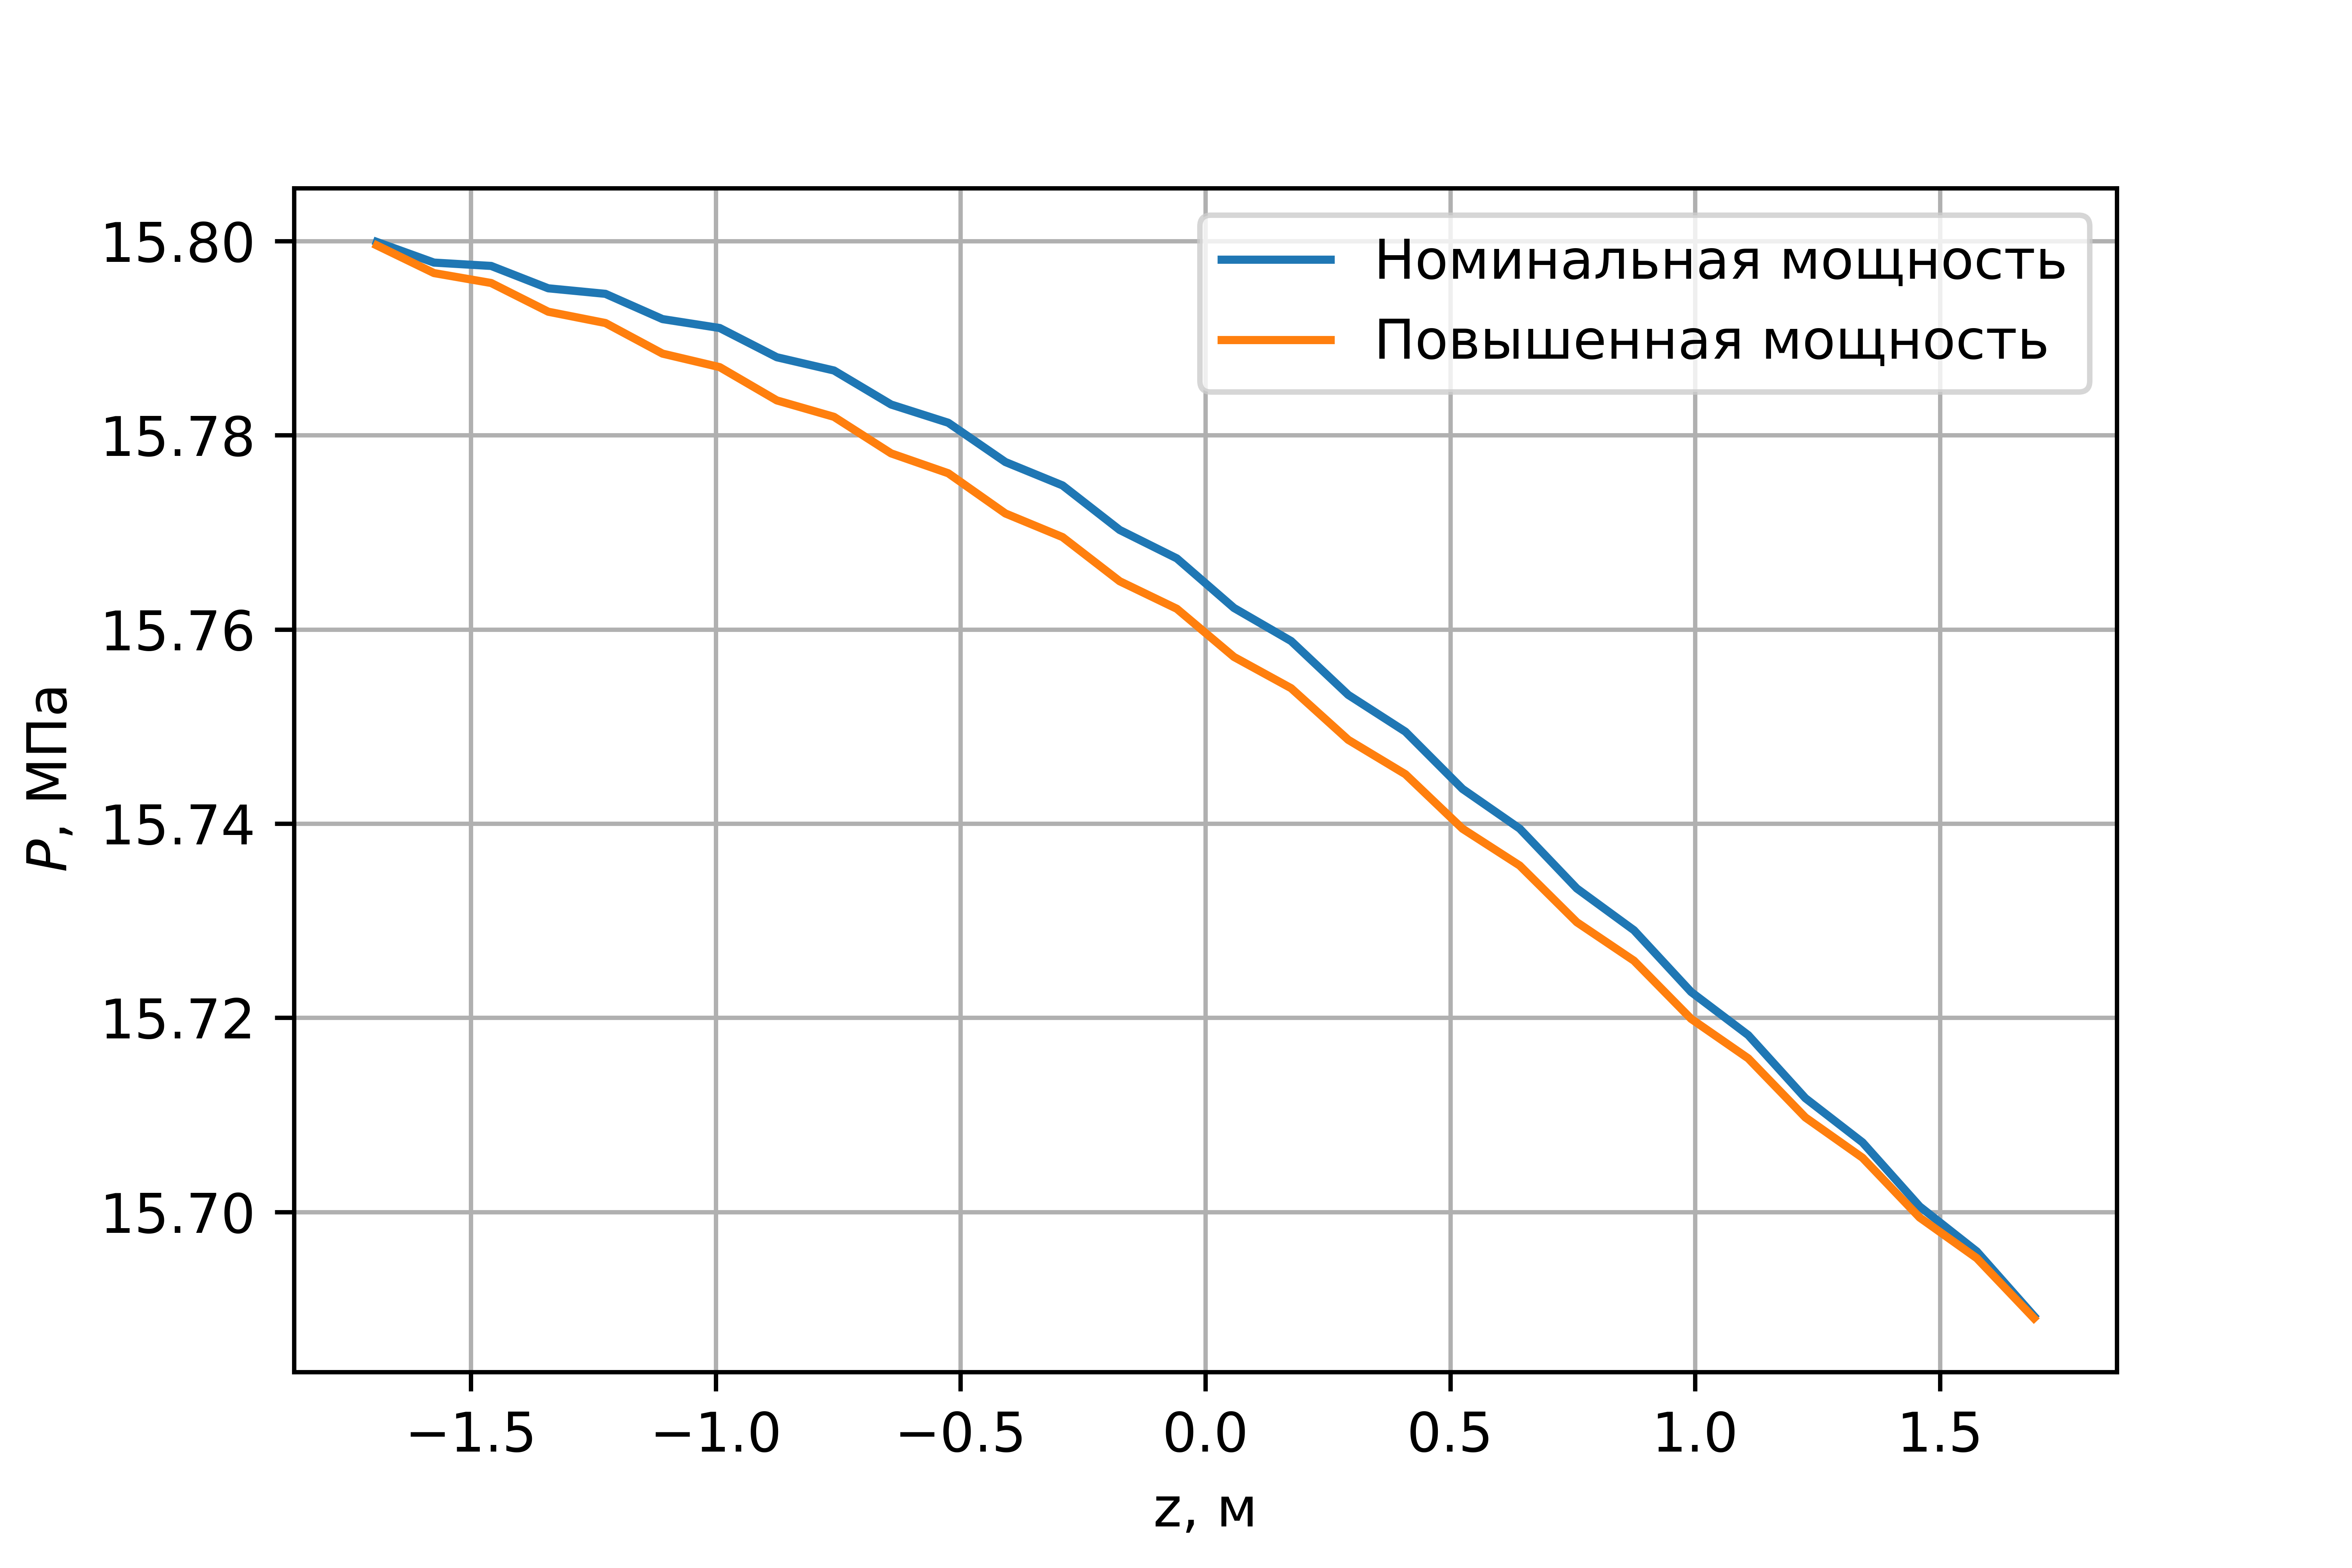
\includegraphics{p_povish_max.png}
		\caption{Распределение давления в кассете с максимальной температурой по высоте АЗ}
		\label{pic:p-povish-max} % название для ссылок внутри кода
	\end{center}
\end{figure}

Из рисунка \ref{pic:podogrev-povish} видно, что при повышении мощности на 5\% подогрев между первой и последней расчетными точками в центральной ТВС поднялся на 1.6 $^\circ C$. На рисунке \ref{pic:podogrev-povish-by-r} представлено распределение подогревов, усредненных по радиальным группам ТВС


\begin{figure}[H]
	\begin{center}
		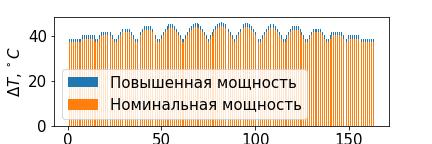
\includegraphics{podogrev_povish.jpg}
		\caption{Распределение подогревов по всем ТВС}
		\label{pic:podogrev-povish} % название для ссылок внутри кода
	\end{center}
\end{figure}

\begin{figure}[H]
	\begin{center}
		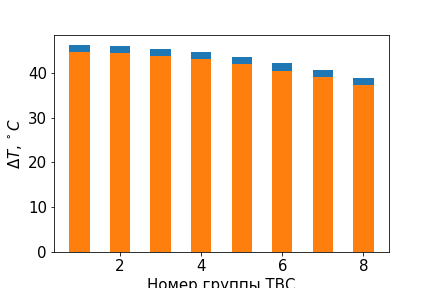
\includegraphics{podogrev_povish_by_r.png}
		\caption{Распределение подогревов по радиальным группам ТВС}
		\label{pic:podogrev-povish-by-r} % название для ссылок внутри кода
	\end{center}
\end{figure}

% TODO: сравнение расходов

\subsection{Расчет теплогидравлических характеристик при отключении одного ГЦН}
Для рассматриваемой установки были проведены расчеты основных теплогидравлических параметров в случае отключения одного из четырех ГЦН. Такой режим работы характерен сниженным уровнем мощности и расхода теплоносителя. При моделировании данного процесса был учтен возникающий при отключении петли возникающий обратный ток теплоносителя. В таком случае в петле, для которой ГЦН отключается, температура теплоносителя на входе снижается. 

С точки зрения расчетной модели для воспроизведения описанных условий была задана пониженная температура $T_{\text{in}}^{\text{low}}=284 \circ C$ на входе в захоложенные петли. Распределение номеров ячеек по четырем петлям ГЦН представлено на рисунке \ref{pic:treton-quarts}. Температура была снижена для ячеек, расположенных в левой верхней области по картограмме \ref{pic:treton-quarts}. При задании во входном файле T\_IN.TXT расчетного модуля «ТРЕТОН». В файл Q6.TXT входное тепловыделение для всех ячеек было снижено до 67\%$Q_{\text{ном}}$ ввиду снижения мощности. 

\begin{figure}[H]
	\begin{center}
		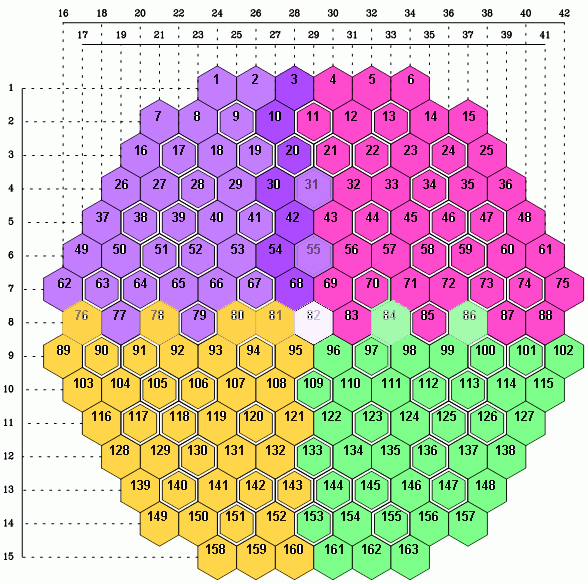
\includegraphics[scale=0.5]{quarts.jpg}
		\caption{Распределение номер ТВС по четырем зонам}
		\label{pic:treton-quarts}
	\end{center}
\end{figure}

По результатам расчета получены максимальные занчения температур топлива, оболочек и теплоносителя, которые представлены в таблице \ref{tabular:t-one-gcn-nominal-compare}

\begin{table}[H]
    \caption{Максимальные температуры теплоносителя, топлива и оболочки твэлов при работе РУ на номинальной и повышенной мощности}
    \begin{center}
        \begin{tabular}{|l|c|c|}
        \toprule
        Тепловая мощность, МВт & 2903 & 1945 \\
        \midrule
        \hline
        Максимальная температура теплоносителя, $\circ C$ & 332.5 & 324.45  \\ 
        \hline
        Запас до кипения теплоносителя, $\circ C$ & 13.9 &  22 \\
        \hline
        Максимальная температура топлива, $\circ C$ & 1452 & 1202.2  \\
        \hline
        Максимальная температура внешней оболочки & 346.46 & 335.3 \\
        \hline
        Максимальная температура внутренней оболочки & 381.3 & 361.5 \\
        \hline
        Запас до кипения теплоносителя вблизи оболоки & 0.04 & 11.2 \\
        \bottomrule
        \end{tabular}
		\label{tabular:t-one-gcn-nominal-compare}
    \end{center}
\end{table}

\begin{figure}[H]
	\begin{center}
		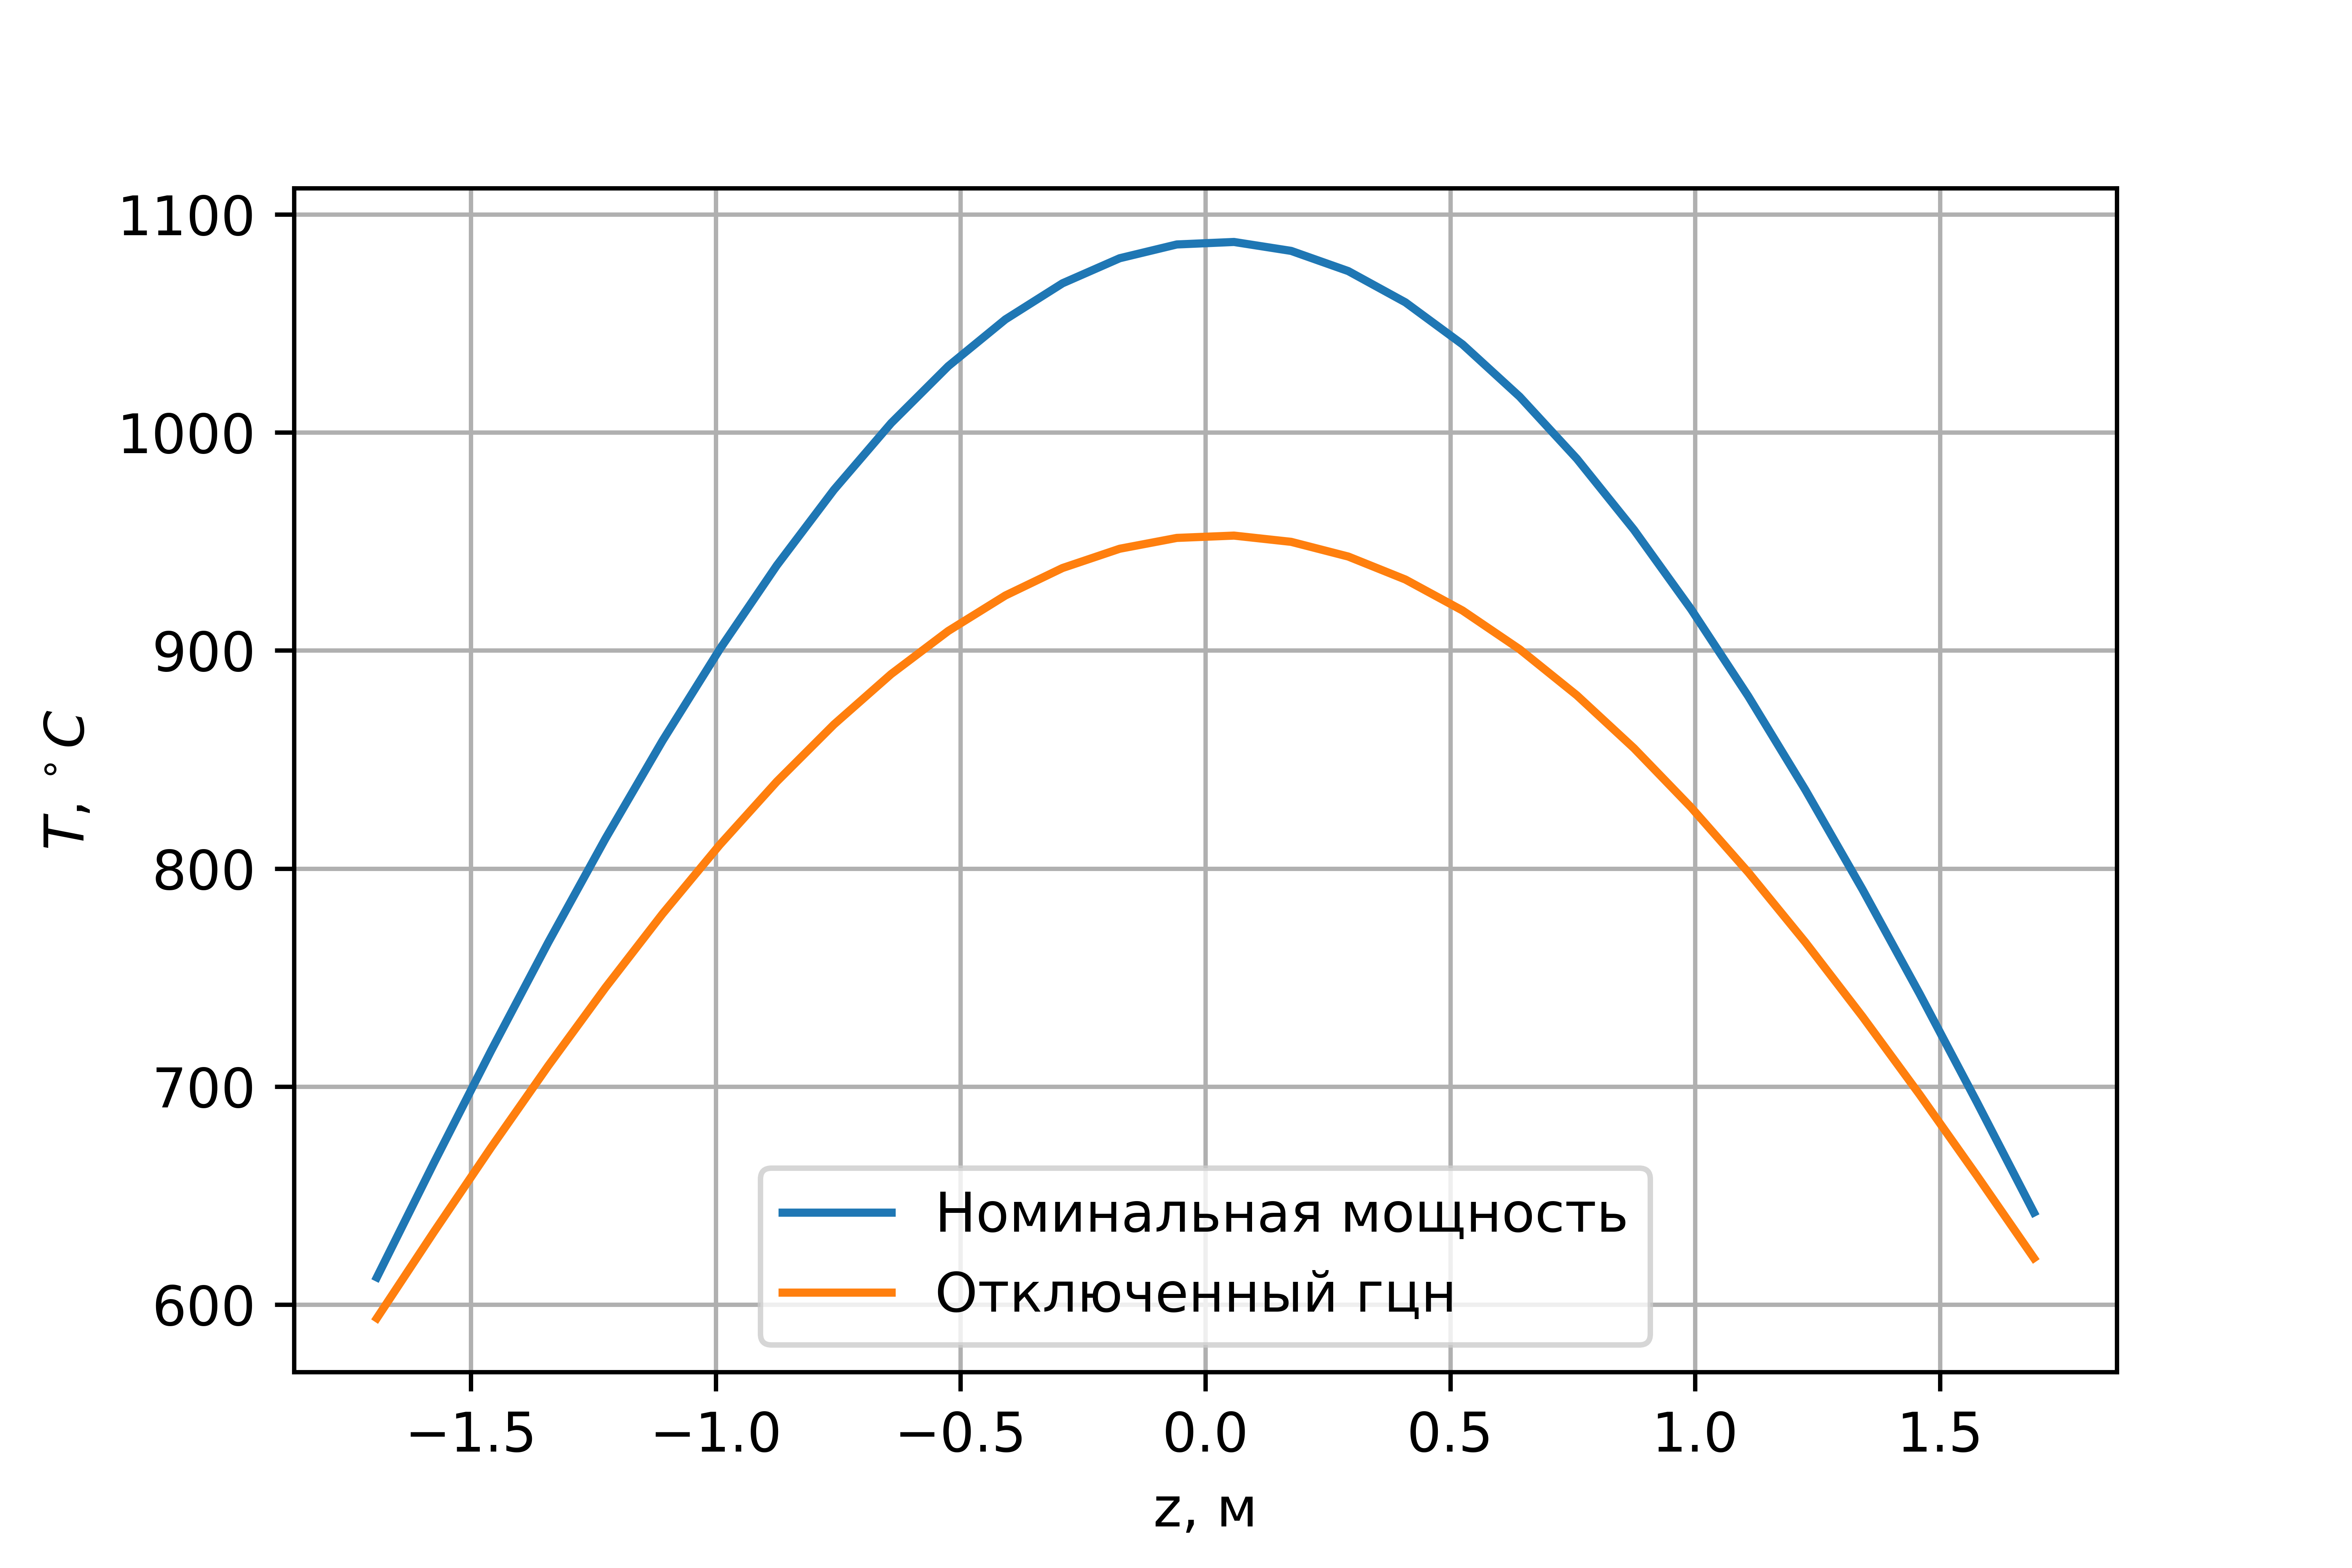
\includegraphics{treton_t_fuel_one_gcn_compare.png}
		\caption{Распределение температуры топлива по высоте АЗ}
		\label{pic:treton-t-fuel-one-gcn-compare} % название для ссылок внутри кода
	\end{center}
\end{figure}

\begin{figure}[H]
	\begin{center}
		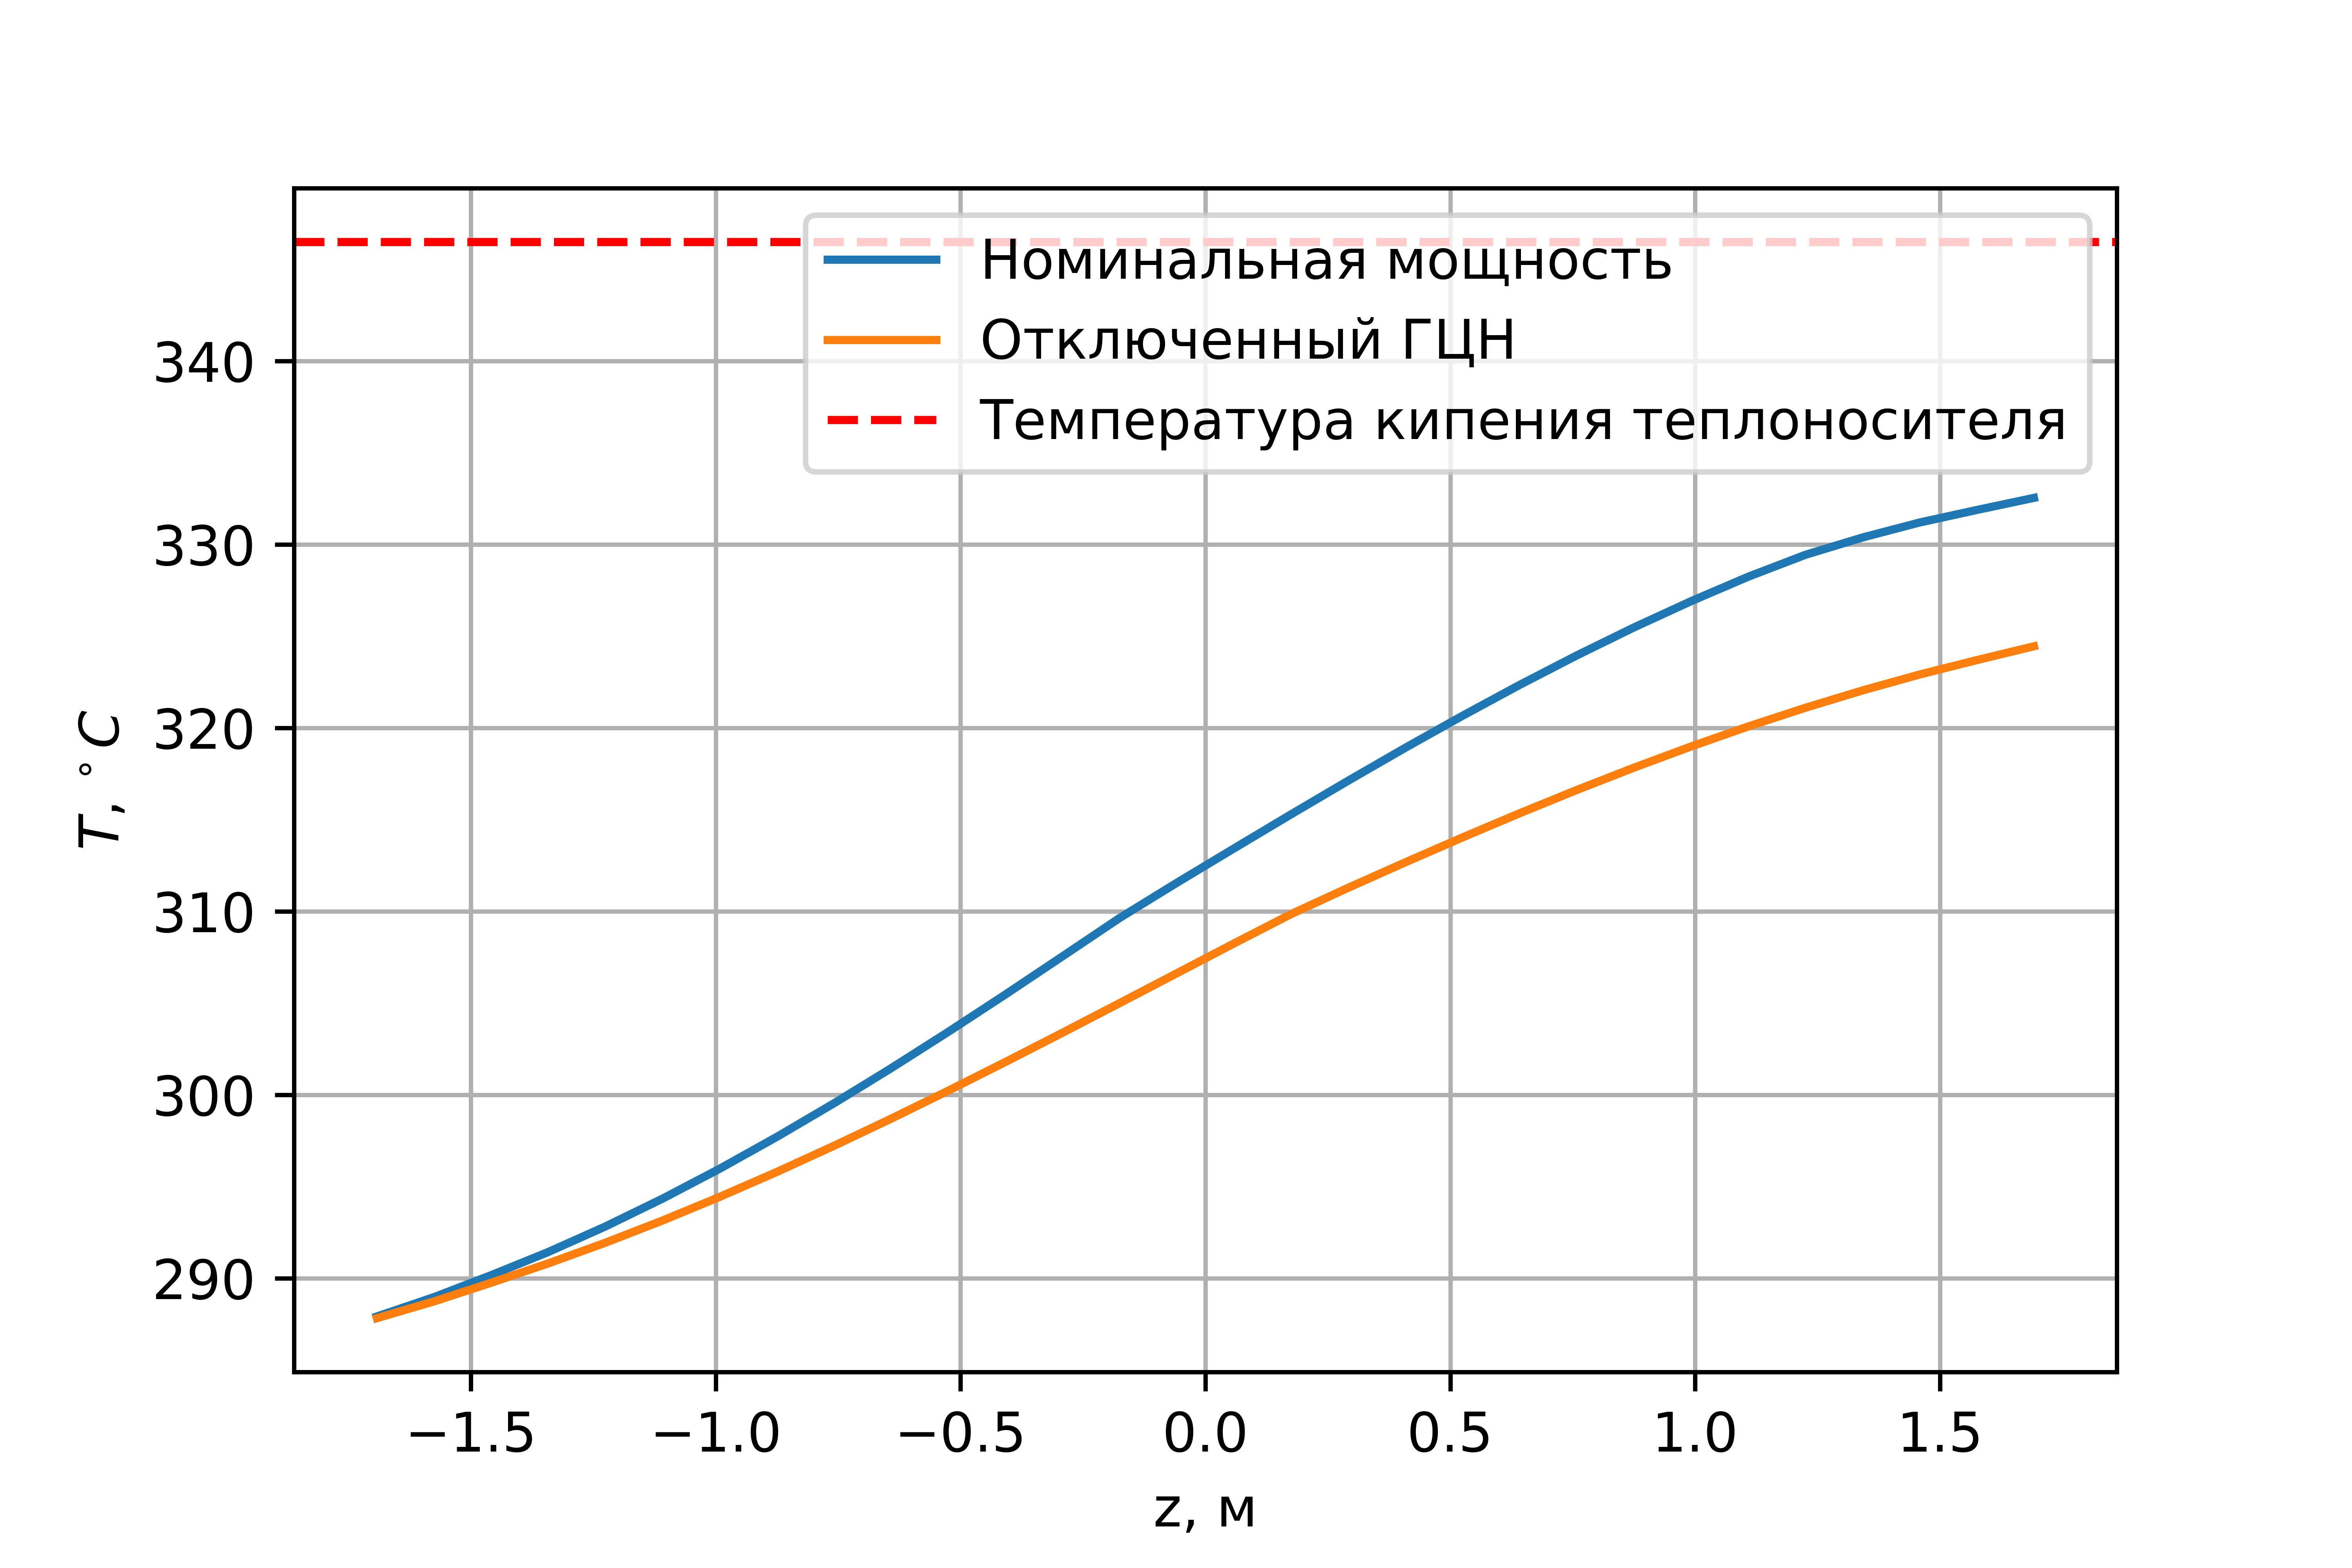
\includegraphics{treton_t_tepl_one_gcn_compare.png}
		\caption{Распределение температуры теплоносителя по высоте АЗ}
		\label{pic:treton-t-tepl-one-gcn-compare} % название для ссылок внутри кода
	\end{center}
\end{figure}

\begin{figure}[H]
	\begin{center}
		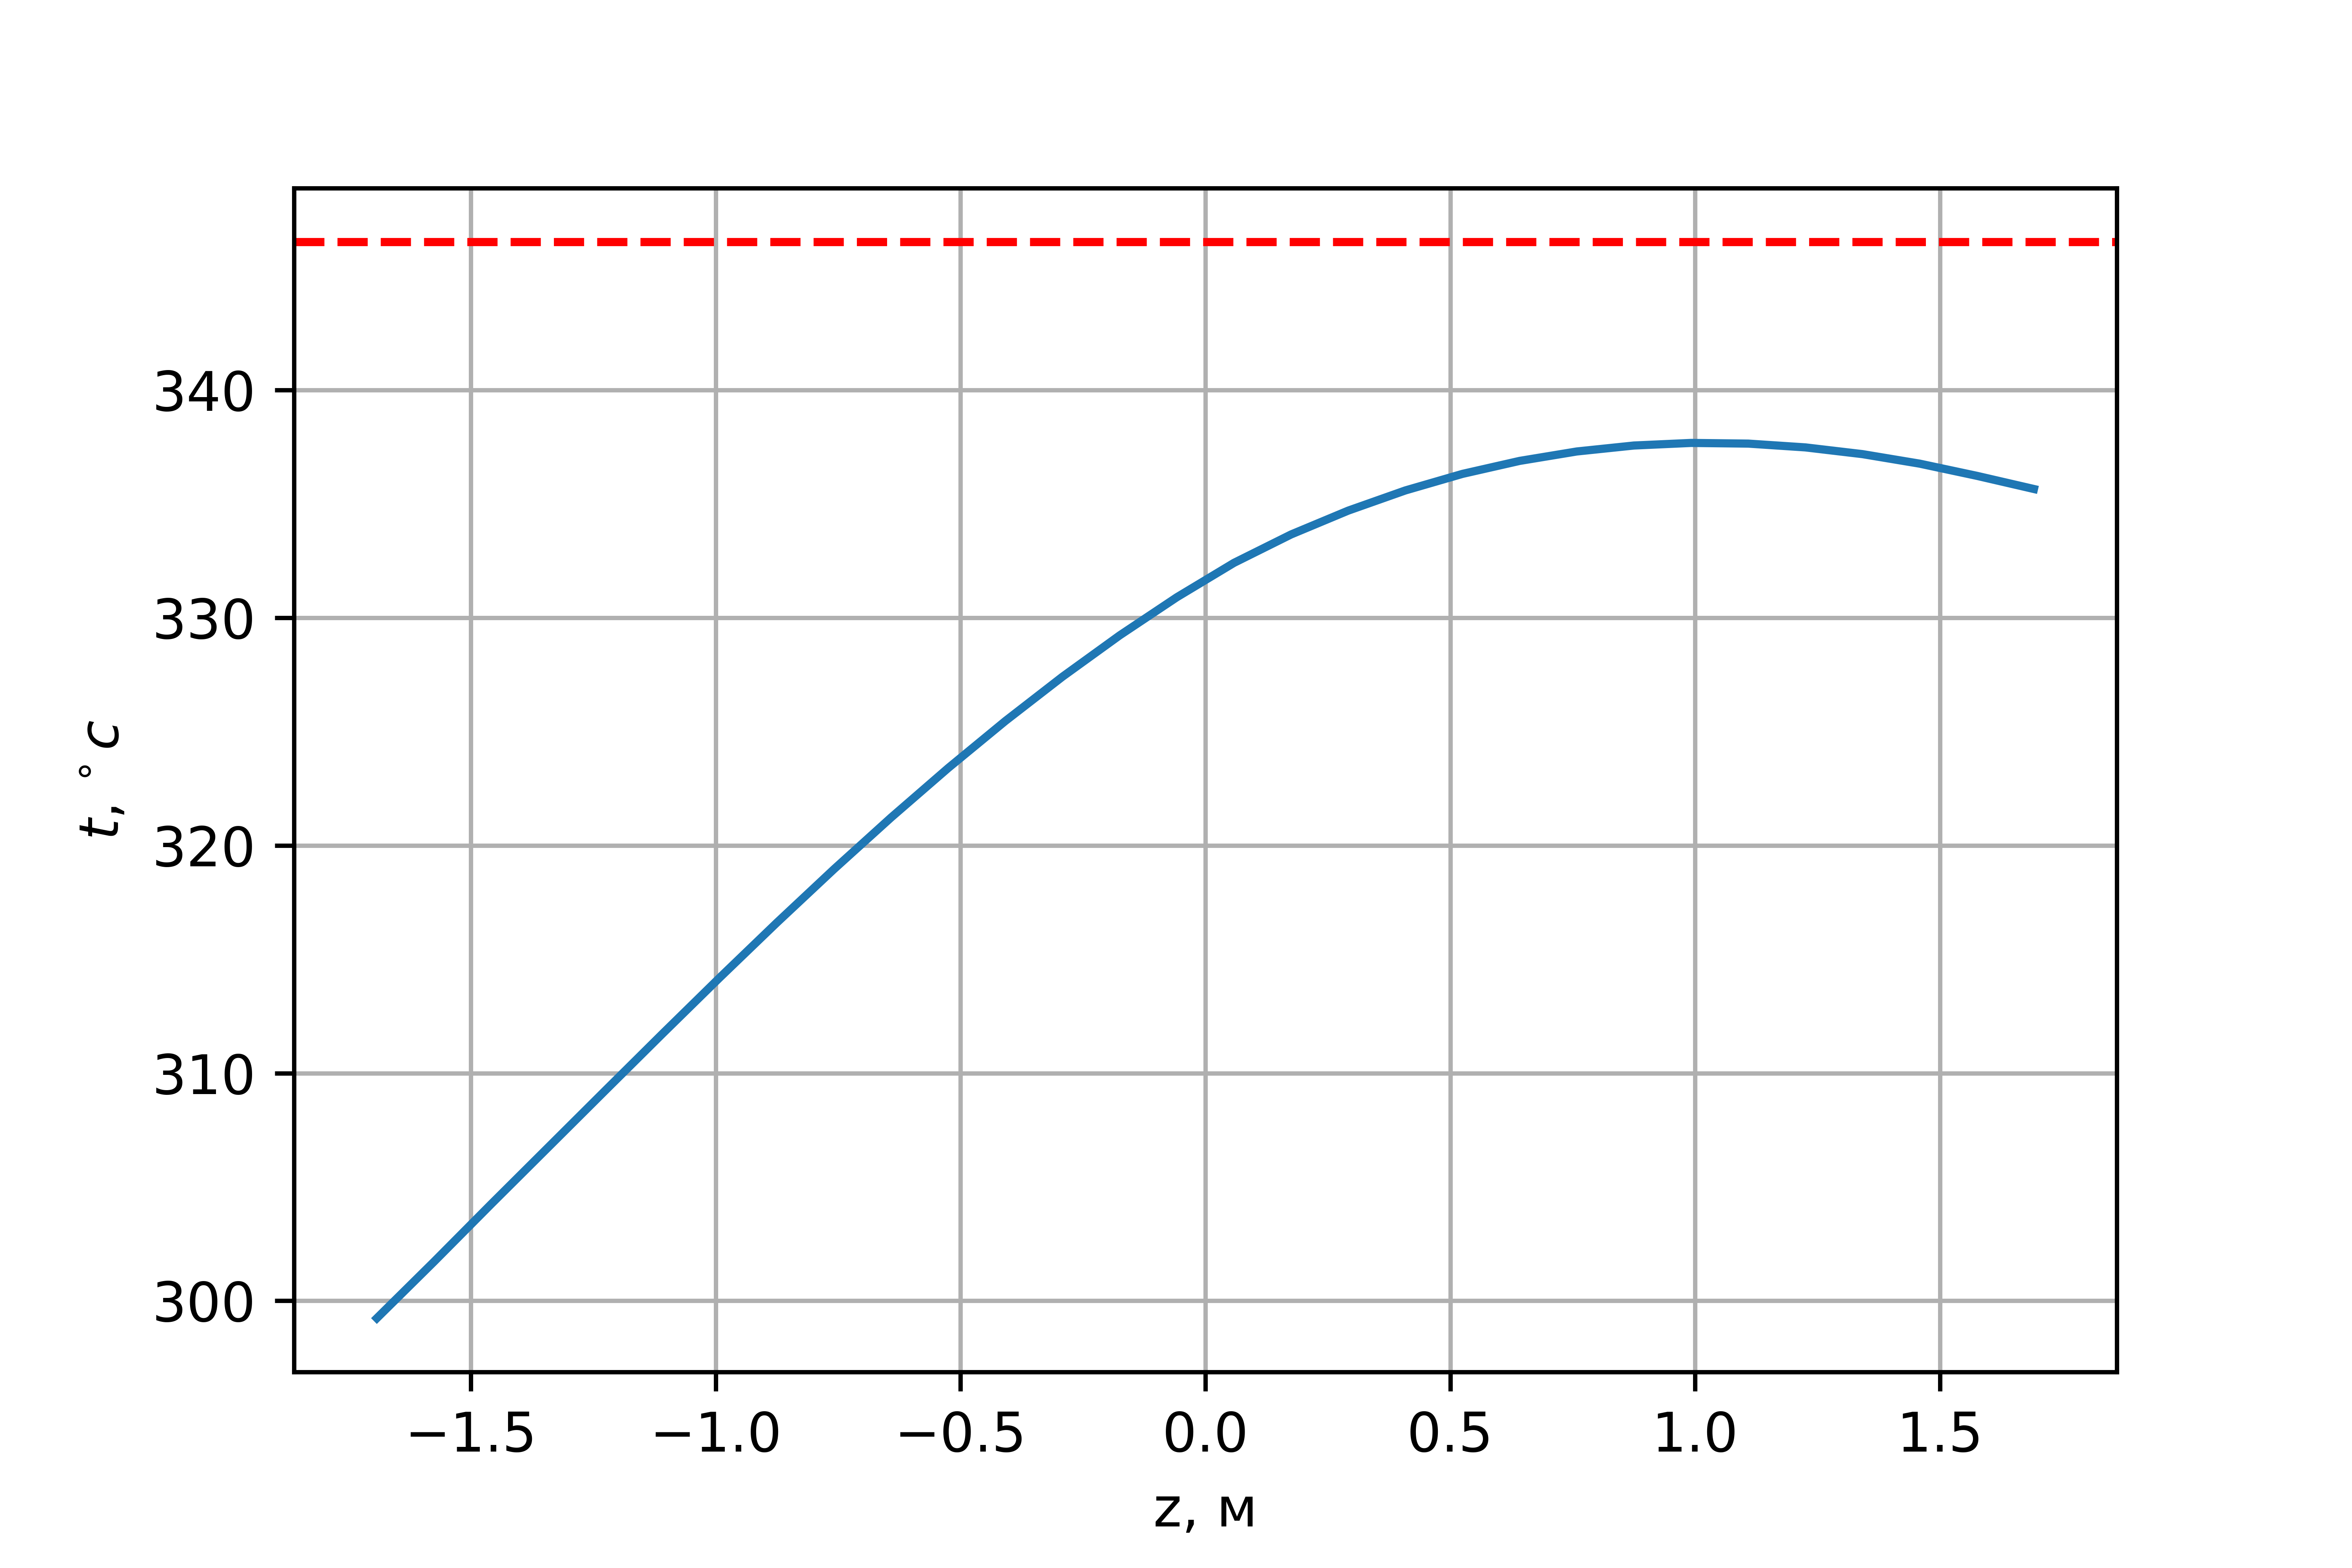
\includegraphics{treton_one_gcn_obl_naruj_max.png}
		\caption{Распределение температуры наруженй оболочки твэлов по высоте для кассеты с максимальной температурой теплоносителя}
		\label{pic:treton-one-gcn-obl-naruj-max} % название для ссылок внутри кода
	\end{center}
\end{figure}

из \ref{tabular:t-one-gcn-nominal-compare} видно, что при оключении одного из ГЦН наблюдаются снижения максимальных температур и увеличение запаса до кипения. Общий график температур для работы реактора при работе на пониженной мощности в следствие отключения одного из ГЦН представлен на рисунке \ref{pic:treton-one-gcn-obl-tepl-obsh}

\begin{figure}[H]
	\begin{center}
		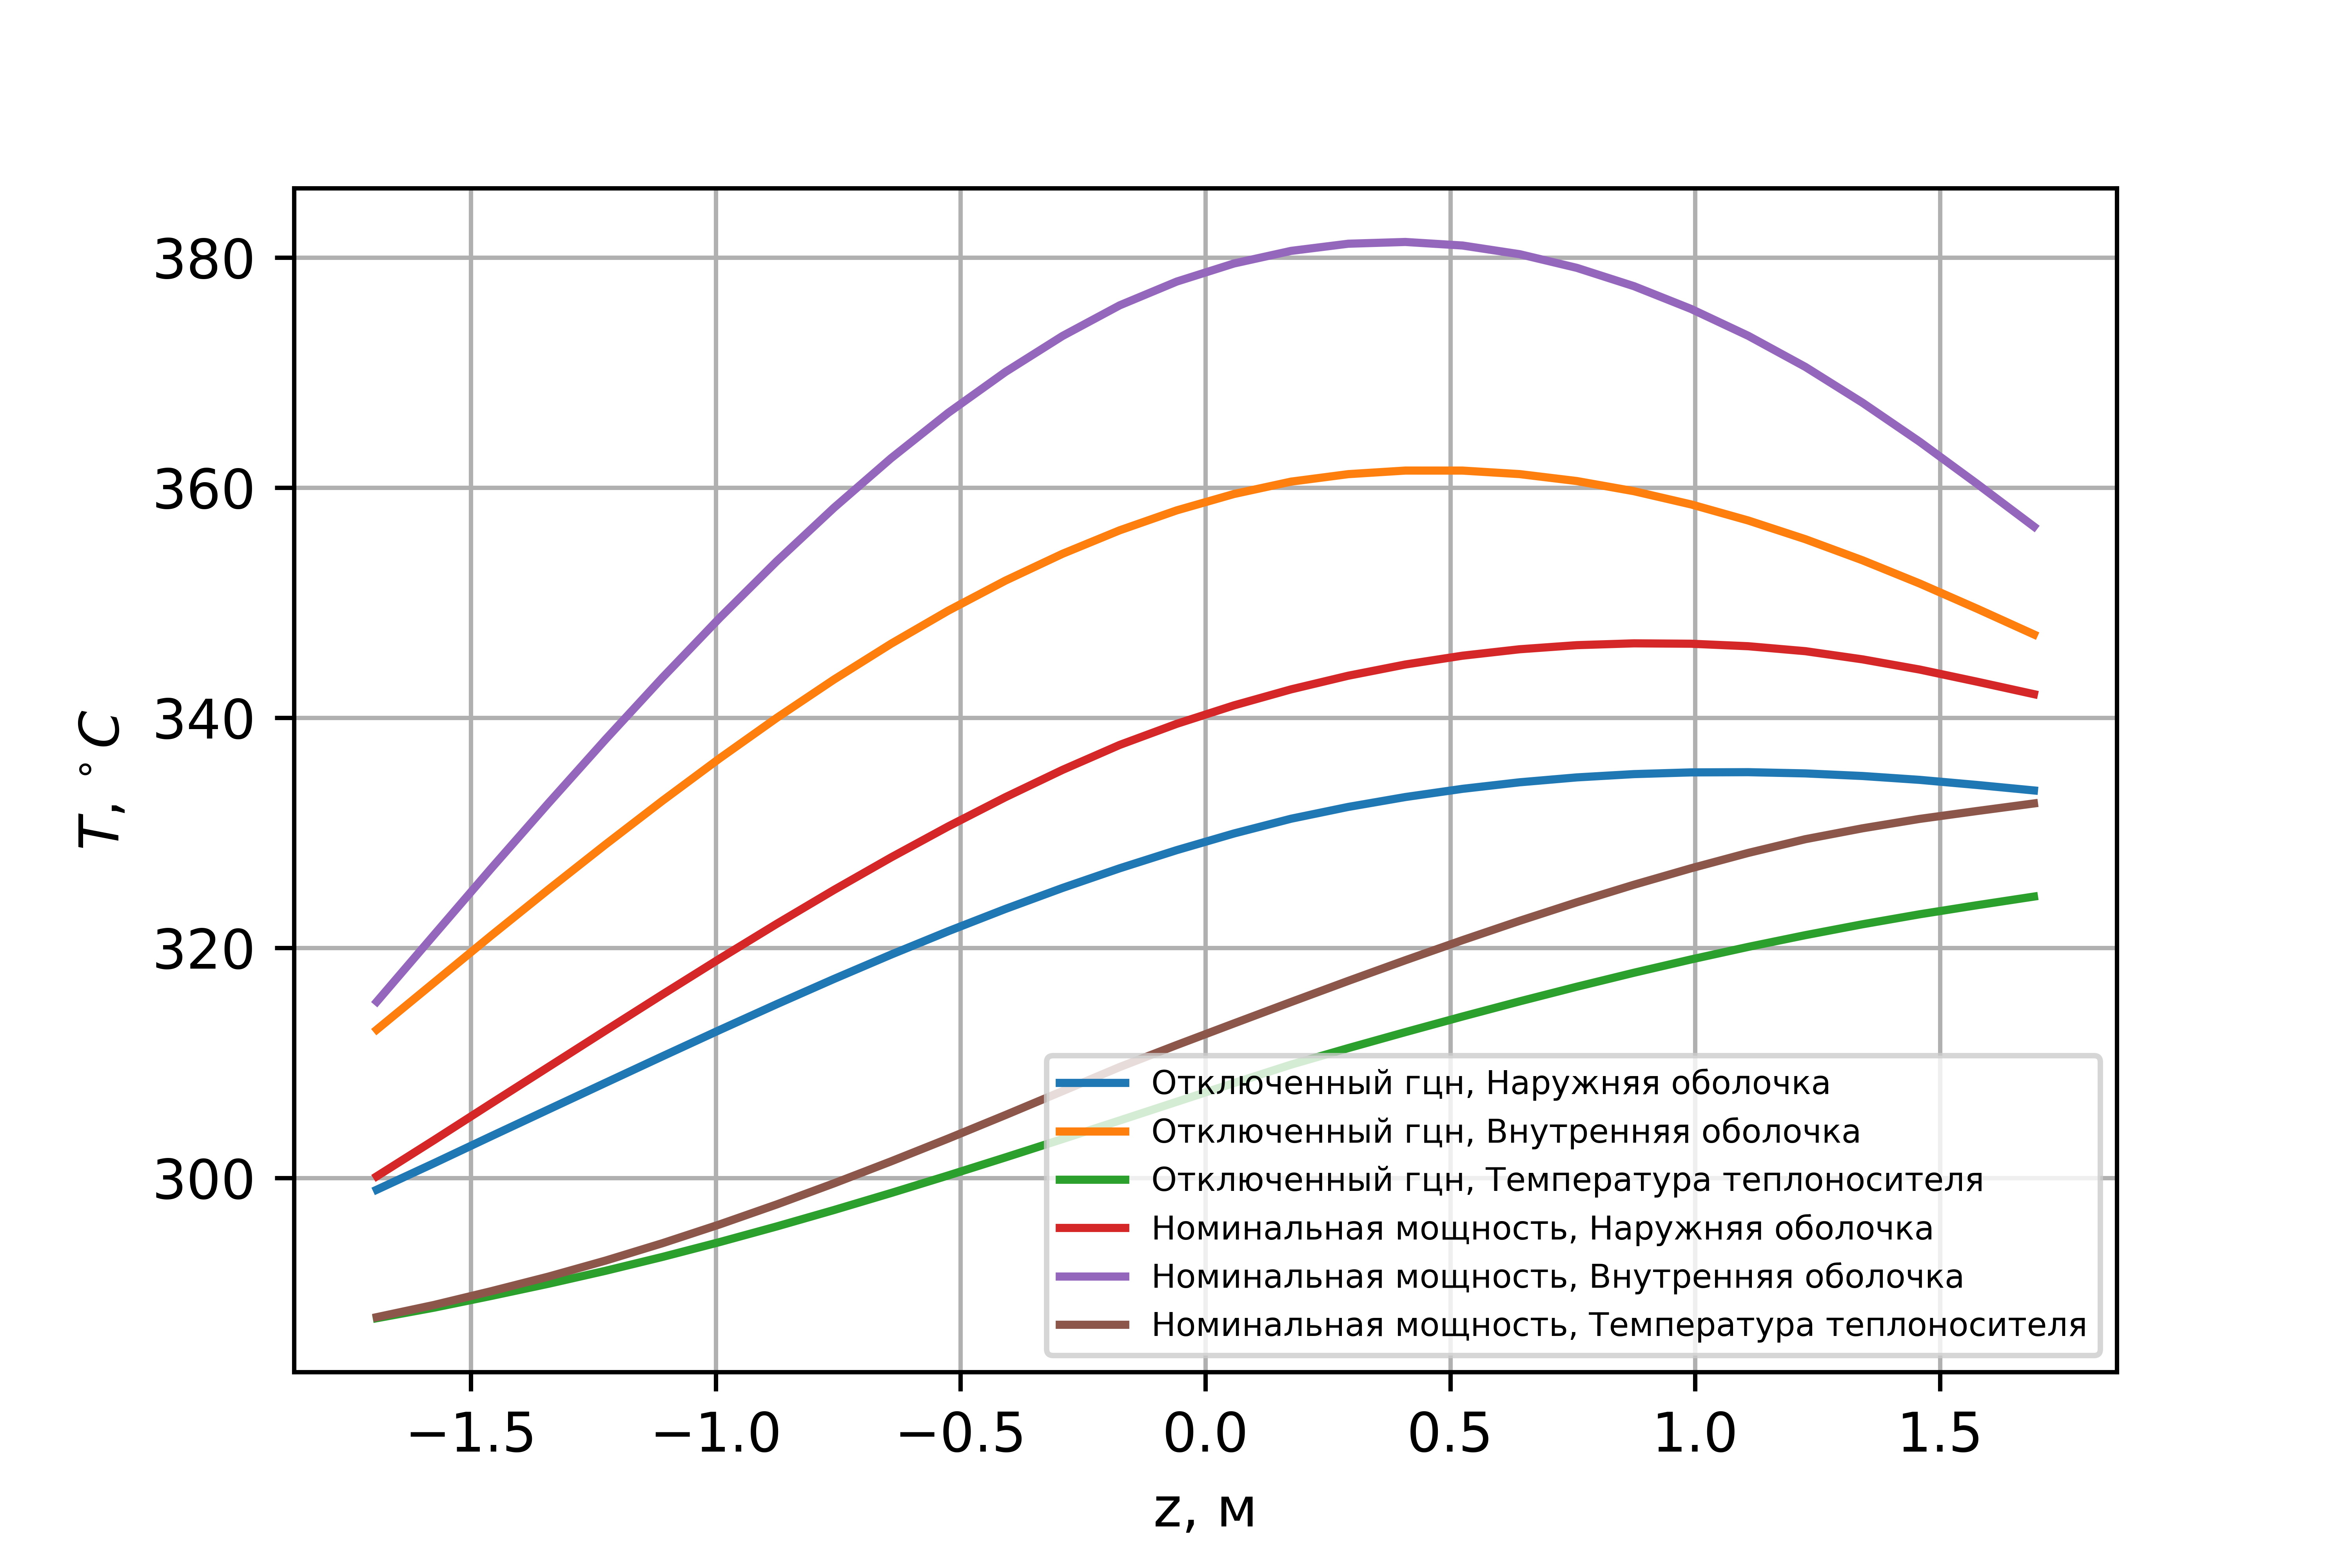
\includegraphics{treton_one_gcn_obl_tepl_obsh.png}
		\caption{Распределение температур по высоте АЗ}
		\label{pic:treton-one-gcn-obl-tepl-obsh} % название для ссылок внутри кода
	\end{center}
\end{figure}

На \ref{pic:podogrev-one-gcn} видно, что при отключении одного ГЦН подогрев в центральной ТВС уменьшился на 8 градусов, средний по всем ТВС подогрев уменьшился на 6.57. 

Для наблюдения возникающей при отключении неравномерности поля температур было построено распределение температуры теплоносителя на входе в активную зоны и на выходе из нее. Соответствующие зависимости представлены на \ref{pic:treton-one-gcn-t-all-cells-z-is-0}, \ref{pic:treton-one-gcn-t-all-cells-z-is-29}. на графиках наблюдается заметный перекос и захолаживание температурного поля в области отключенной петли, возникающий в следствие неравномерности энерговыделения. Для оценки максимального эффекта от неравномерности энерговыделения было построено распределение температуры теплоносителя по высоте АЗ для второй радиальной группы, соответствующей семи ТВС вокруг центарльного. Такое распределение выбрано в силу того что для центарльной ТВС влияние перекоса на характер зависимости незначительный. Распределение представлено на рисунке \ref{pic:treton-one-gcn-2-radius-T}.

\begin{figure}[H]
	\begin{center}
		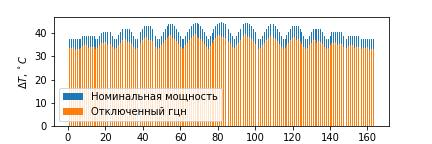
\includegraphics{podogrev_one_gcn.jpg}
		\caption{Распределение подогревов по всем ТВС}
		\label{pic:podogrev-one-gcn} % название для ссылок внутри кода
	\end{center}
\end{figure}

\begin{figure}[H]
	\begin{center}
		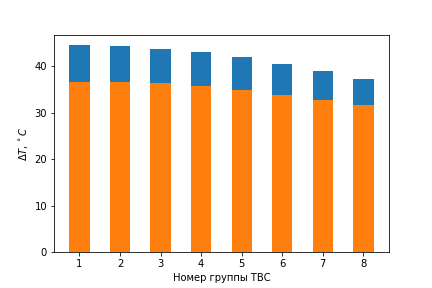
\includegraphics{podogrev_one_gcn_by_r.png}
		\caption{Распределение подогревов по радиальным группам ТВС}
		\label{pic:podogrev-one-gcn-by-r} % название для ссылок внутри кода
	\end{center}
\end{figure}

\begin{figure}[H]
	\begin{center}
		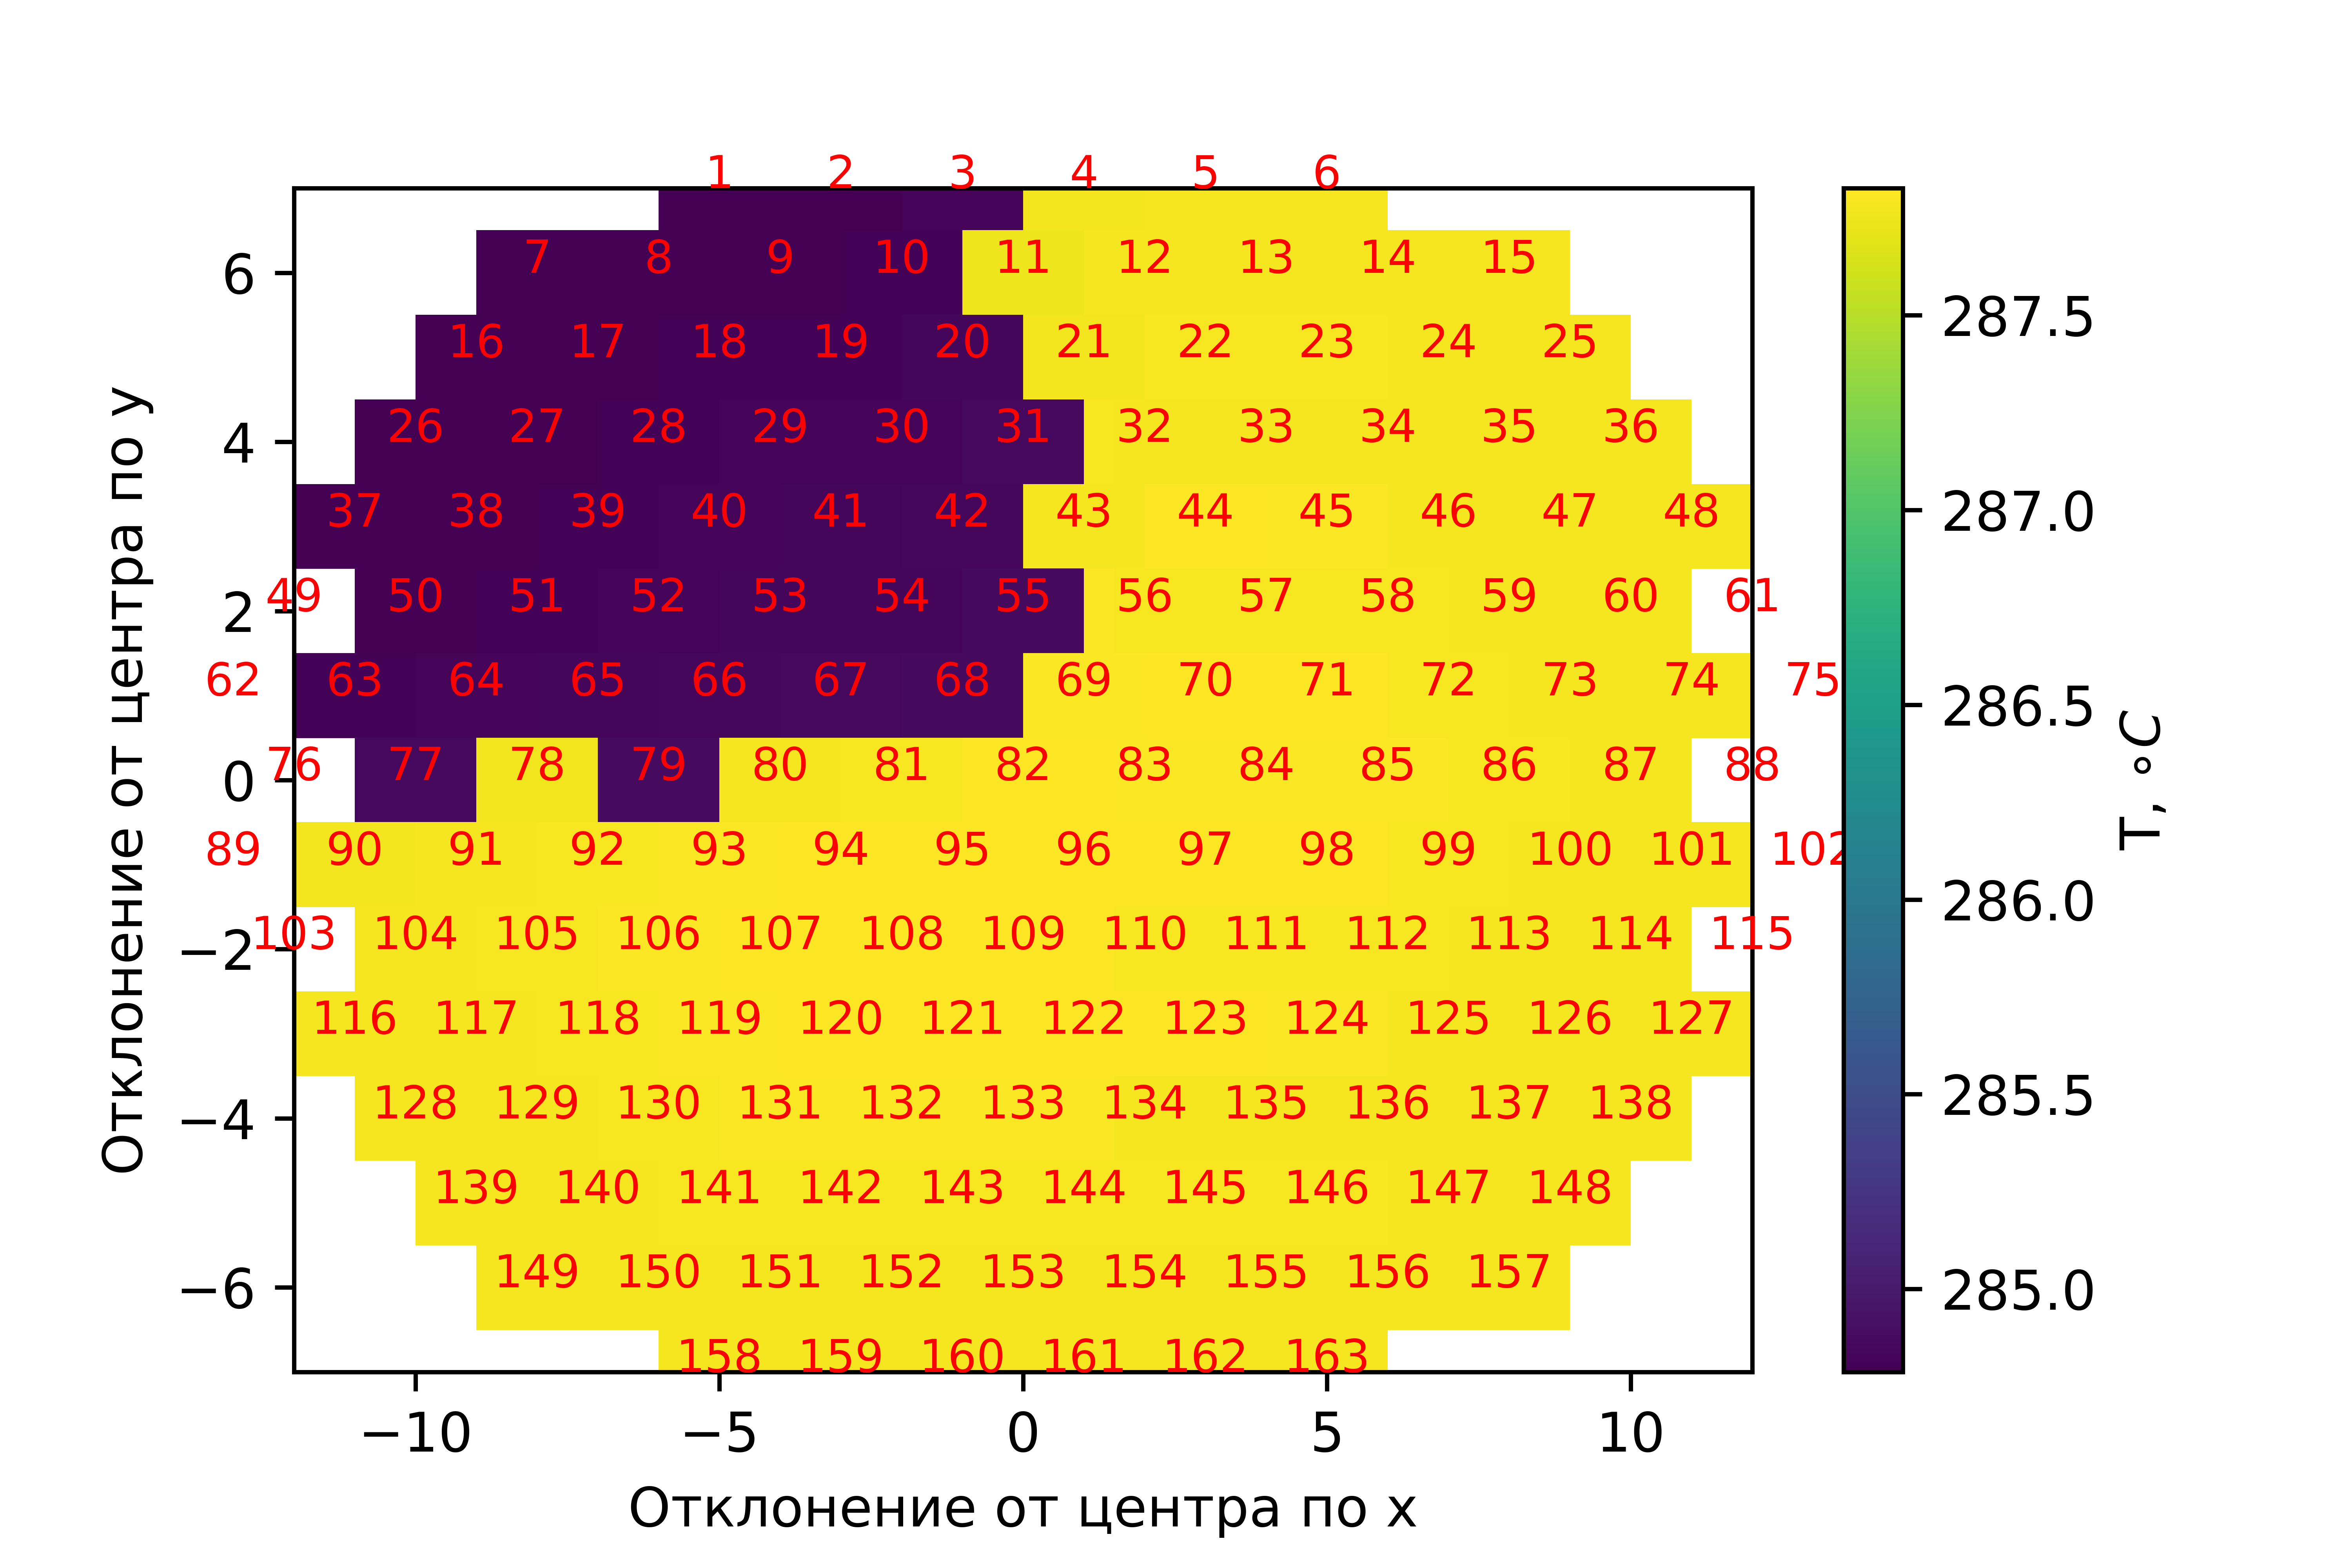
\includegraphics{treton_one_gcn_t_all_cells_z_is_0.png}
		\caption{Распределение температуры теплоносителя по ТВС на входе в АЗ}
		\label{pic:treton-one-gcn-t-all-cells-z-is-0} % название для ссылок внутри кода
	\end{center}
\end{figure}

\begin{figure}[H]
	\begin{center}
		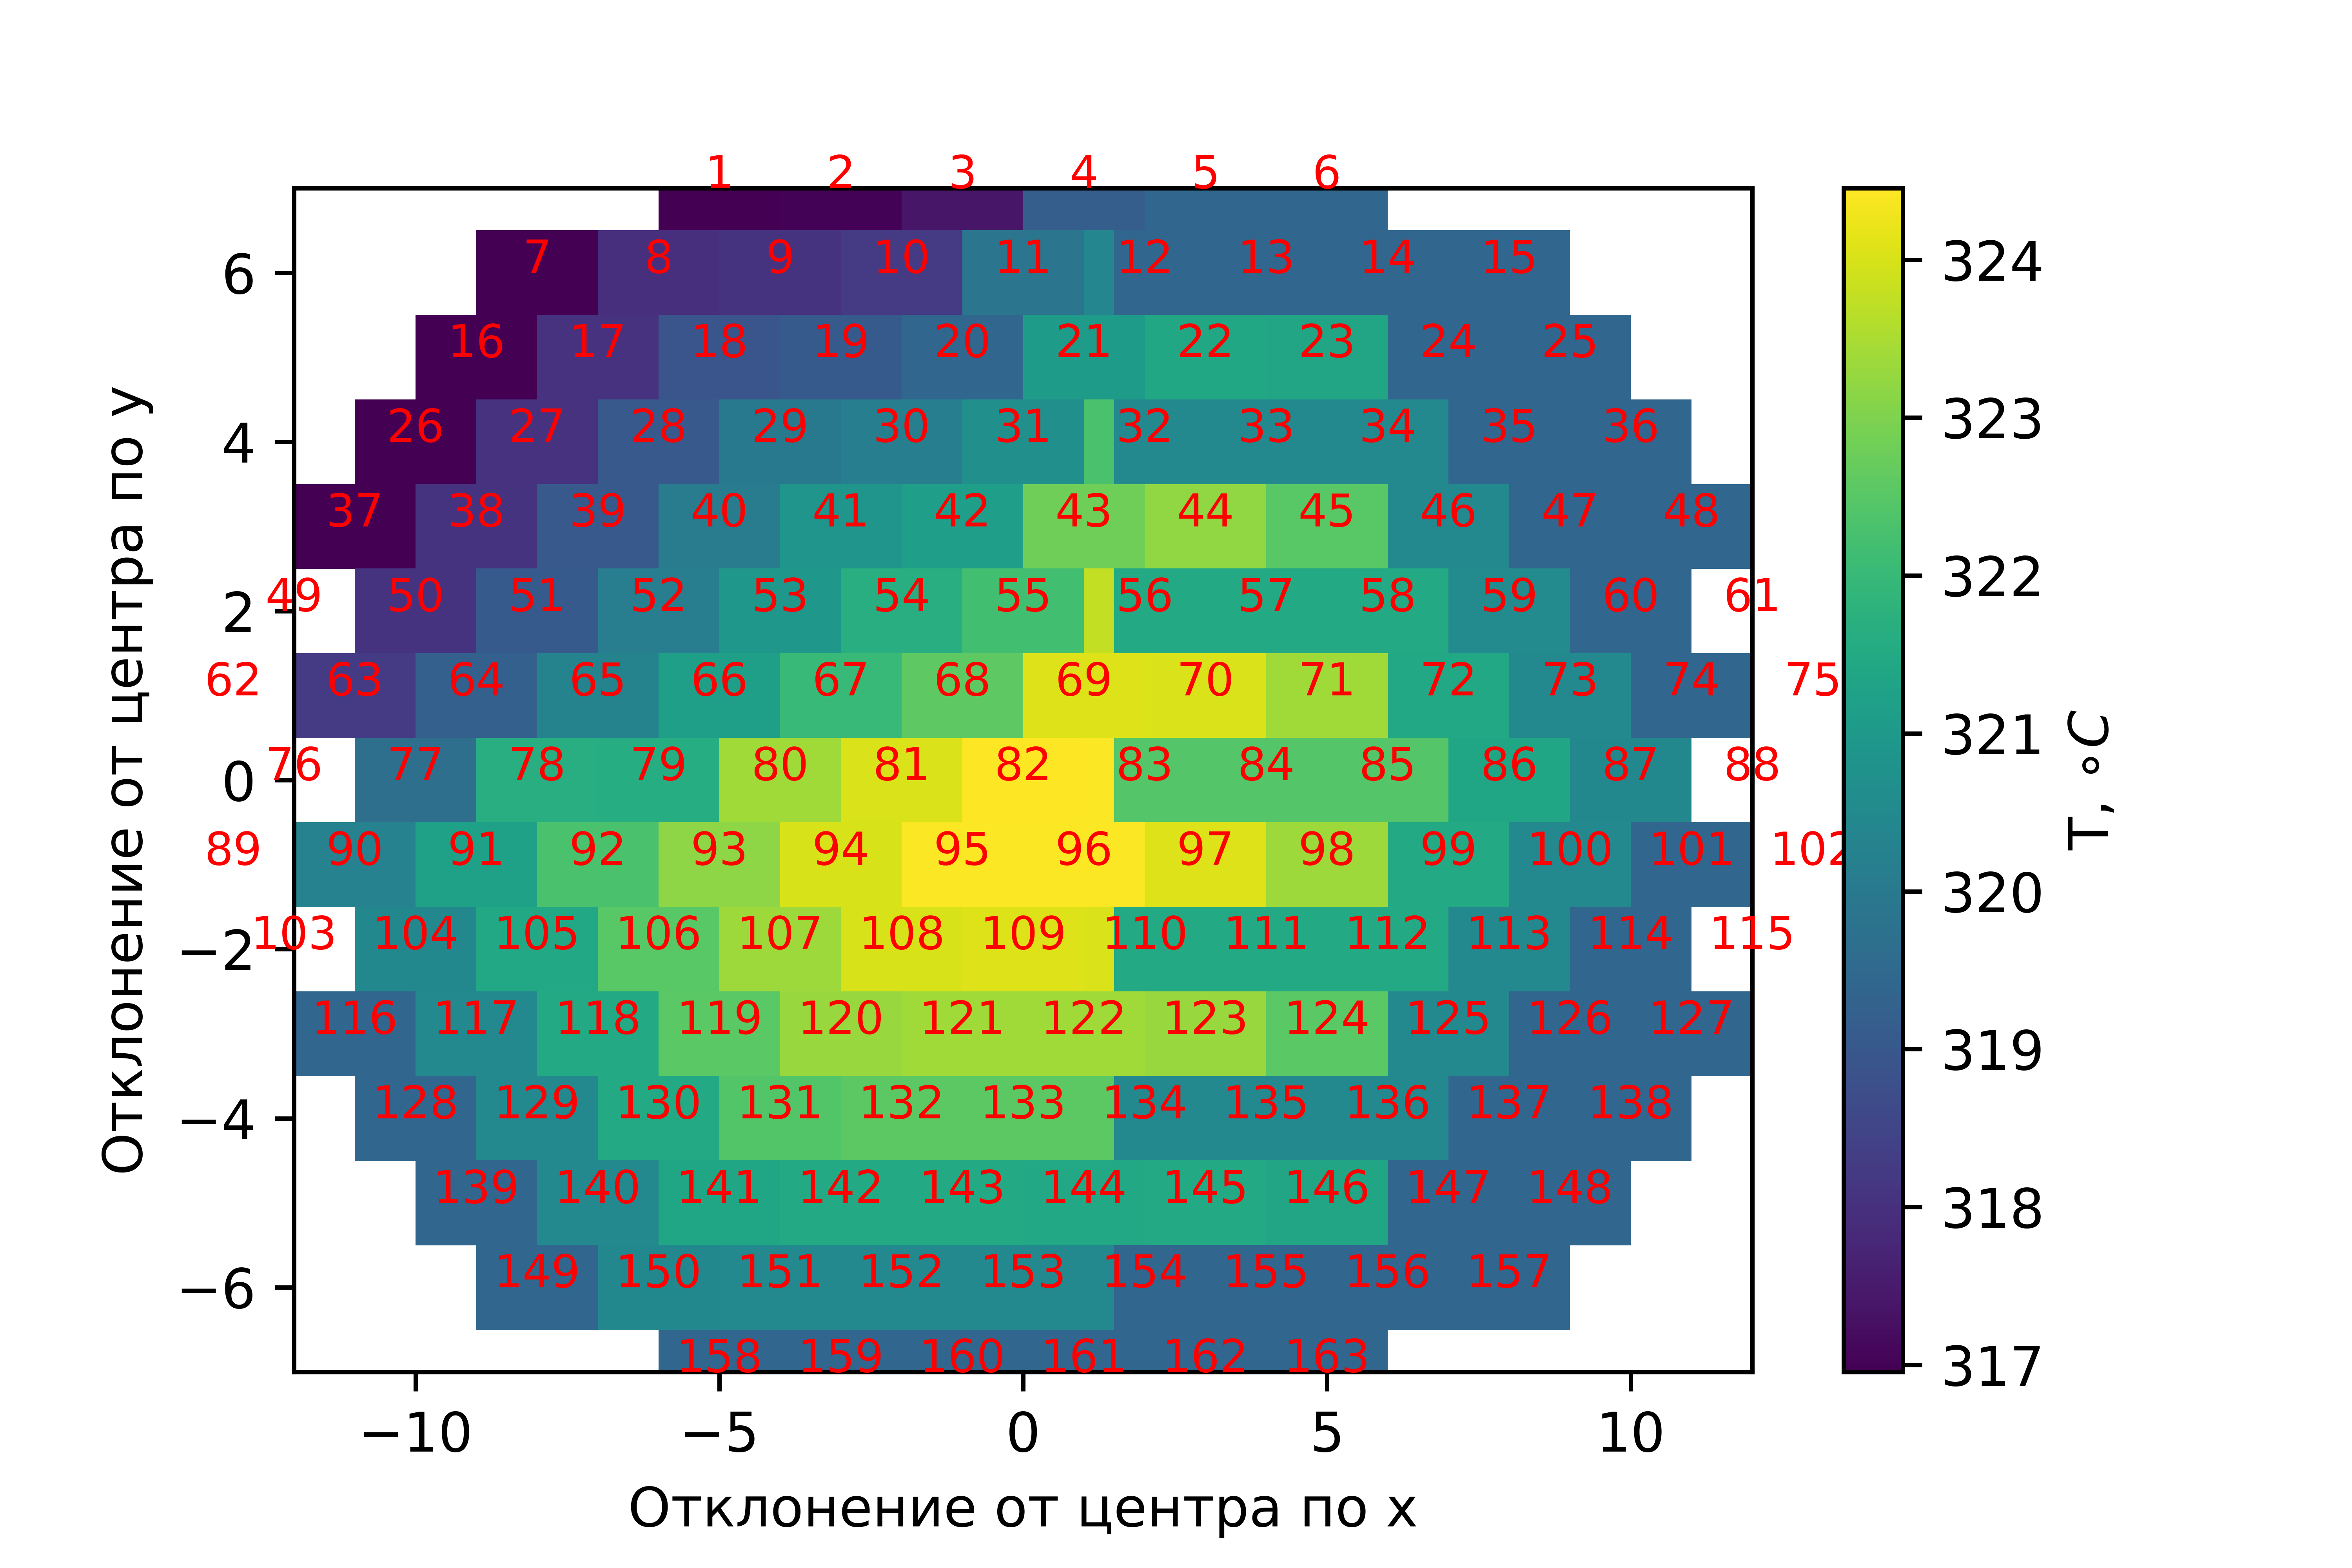
\includegraphics{treton_one_gcn_t_all_cells_z_is_29.png}
		\caption{Распределение температуры теплоносителя по ТВС на выходе из АЗ}
		\label{pic:treton-one-gcn-t-all-cells-z-is-29}
	\end{center}
\end{figure}

\begin{figure}[H]
	\begin{center}
		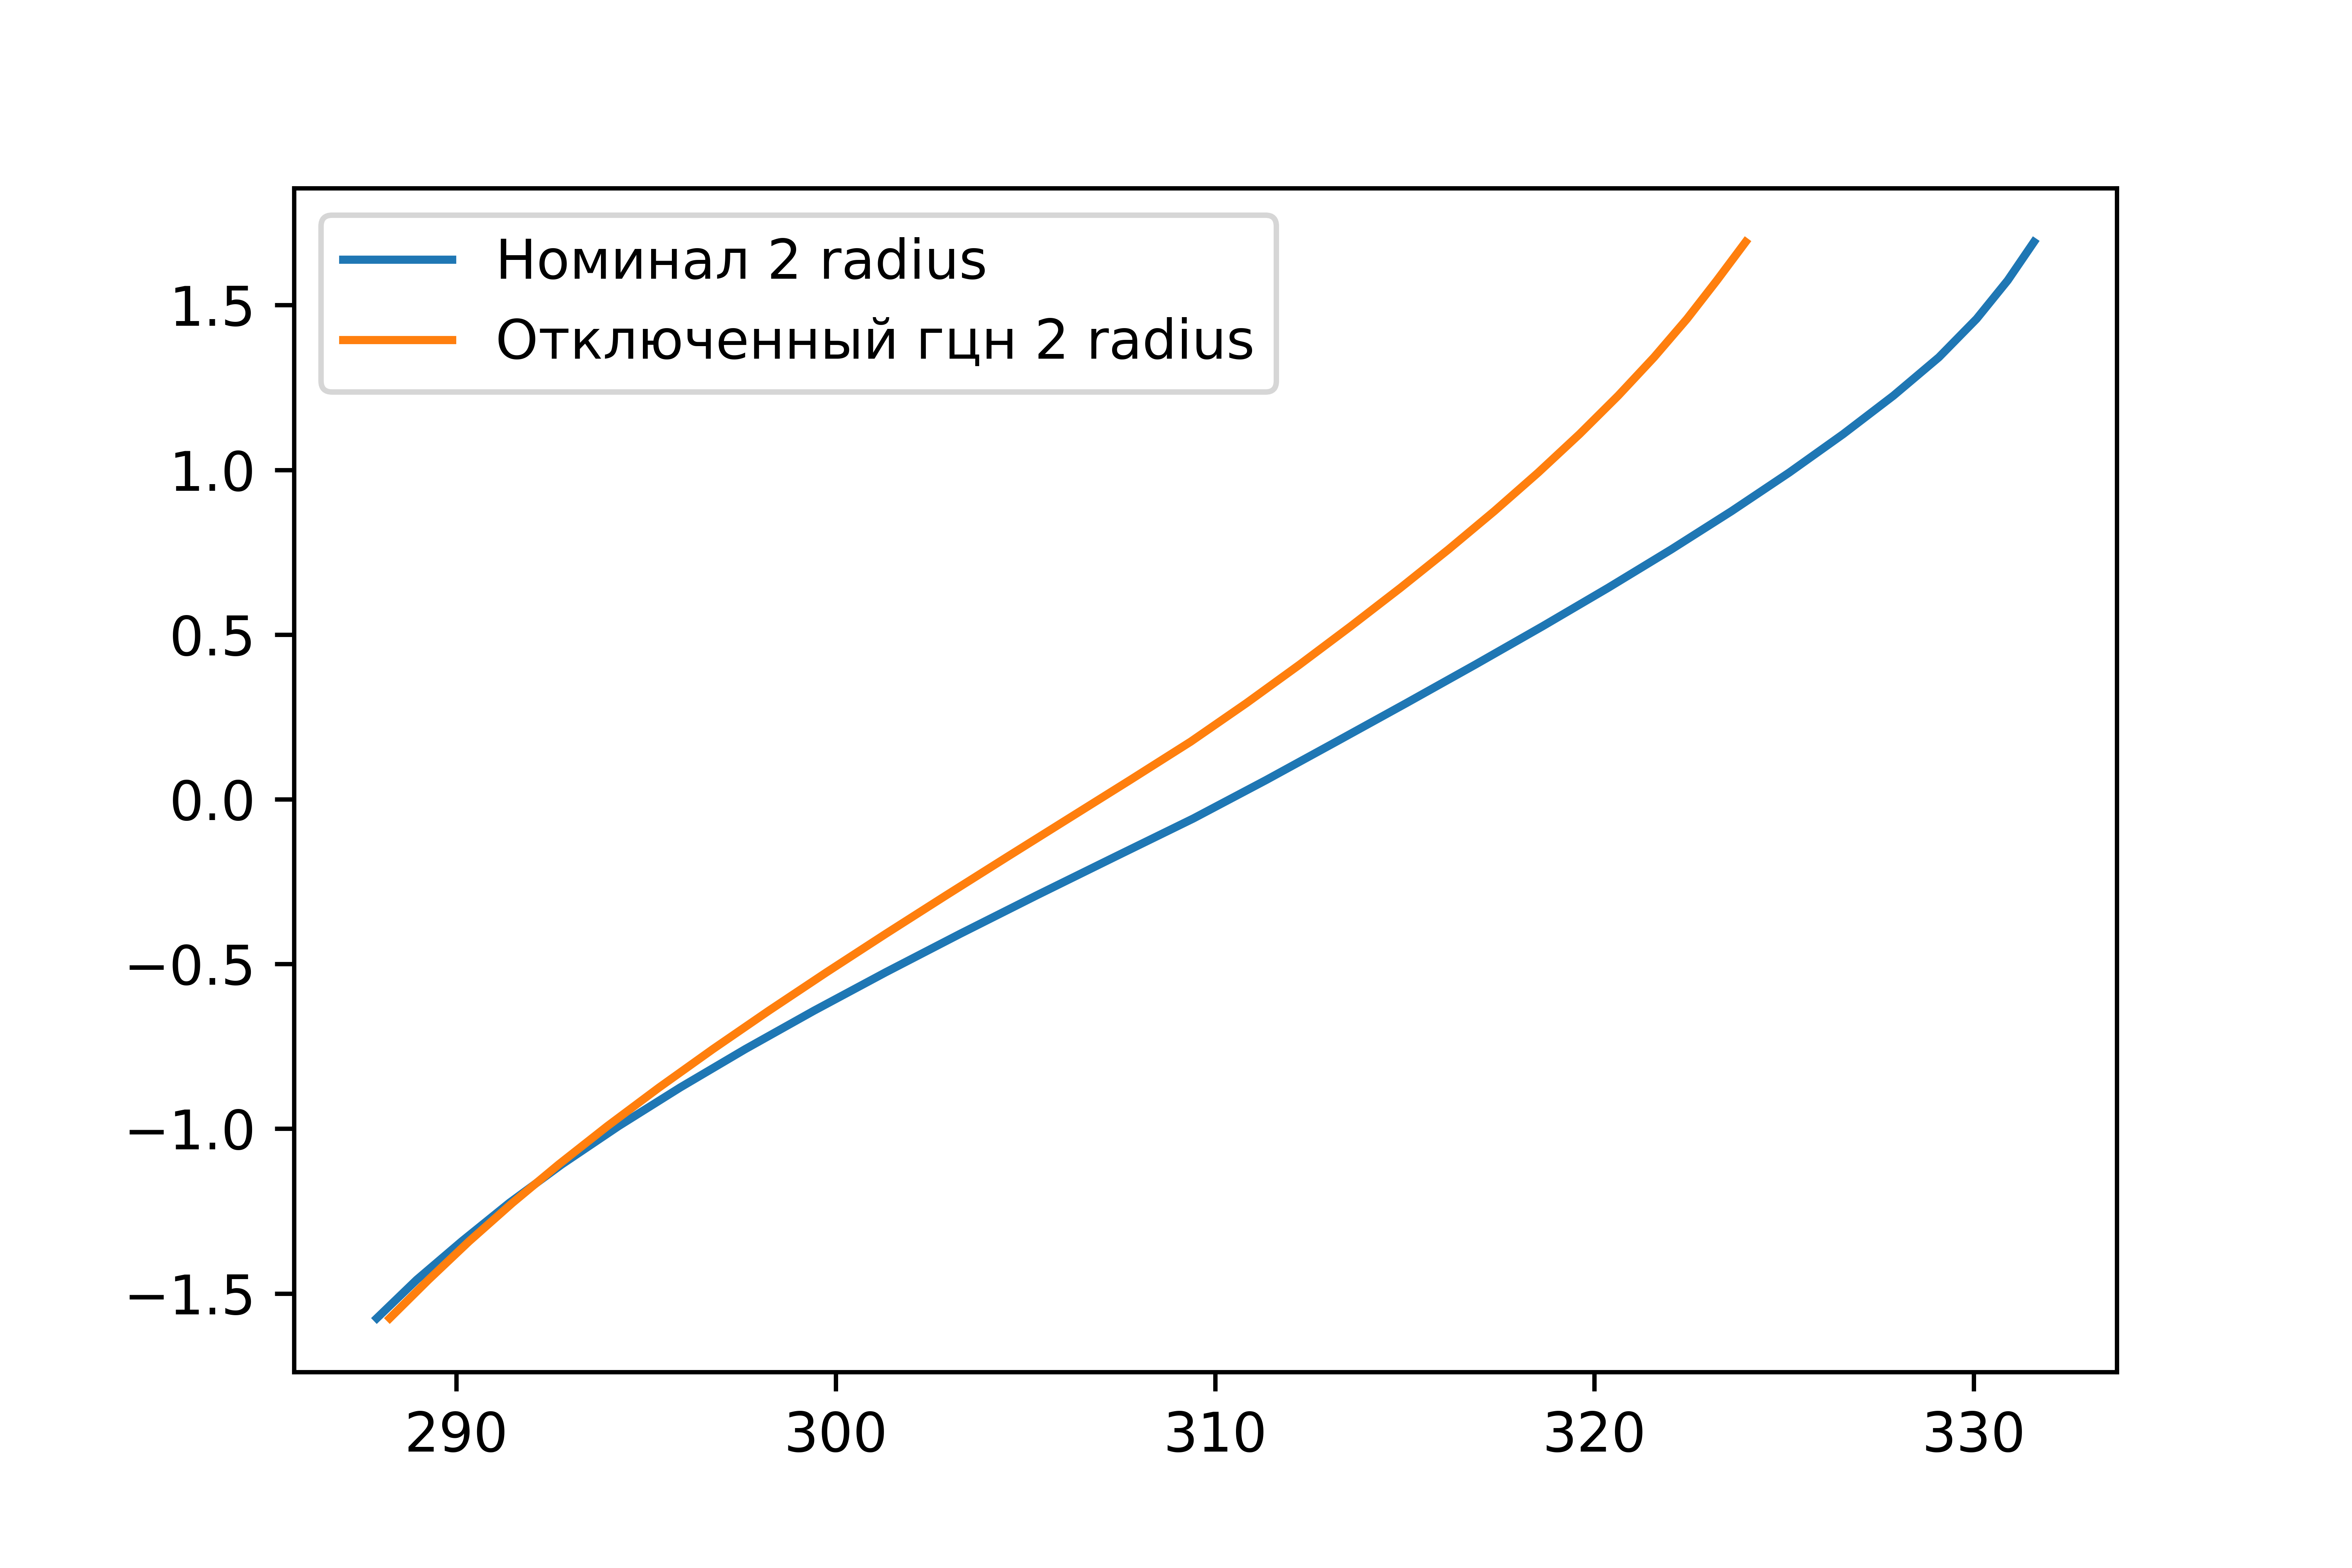
\includegraphics{treton_one_gcn_2_radius_T.png}
		\caption{Распределение температуры теплоносителя по высоте АЗ усредненное по семи ТВС вокруг центральной}
		\label{pic:treton-one-gcn-2-radius-T}
	\end{center}
\end{figure}

% Из \ref{pic:p-one-gcn-max} видно что давление в центральной ТВС уменьшилось на 1.2 КПа

% \begin{figure}[H]
% 	\begin{center}
% 		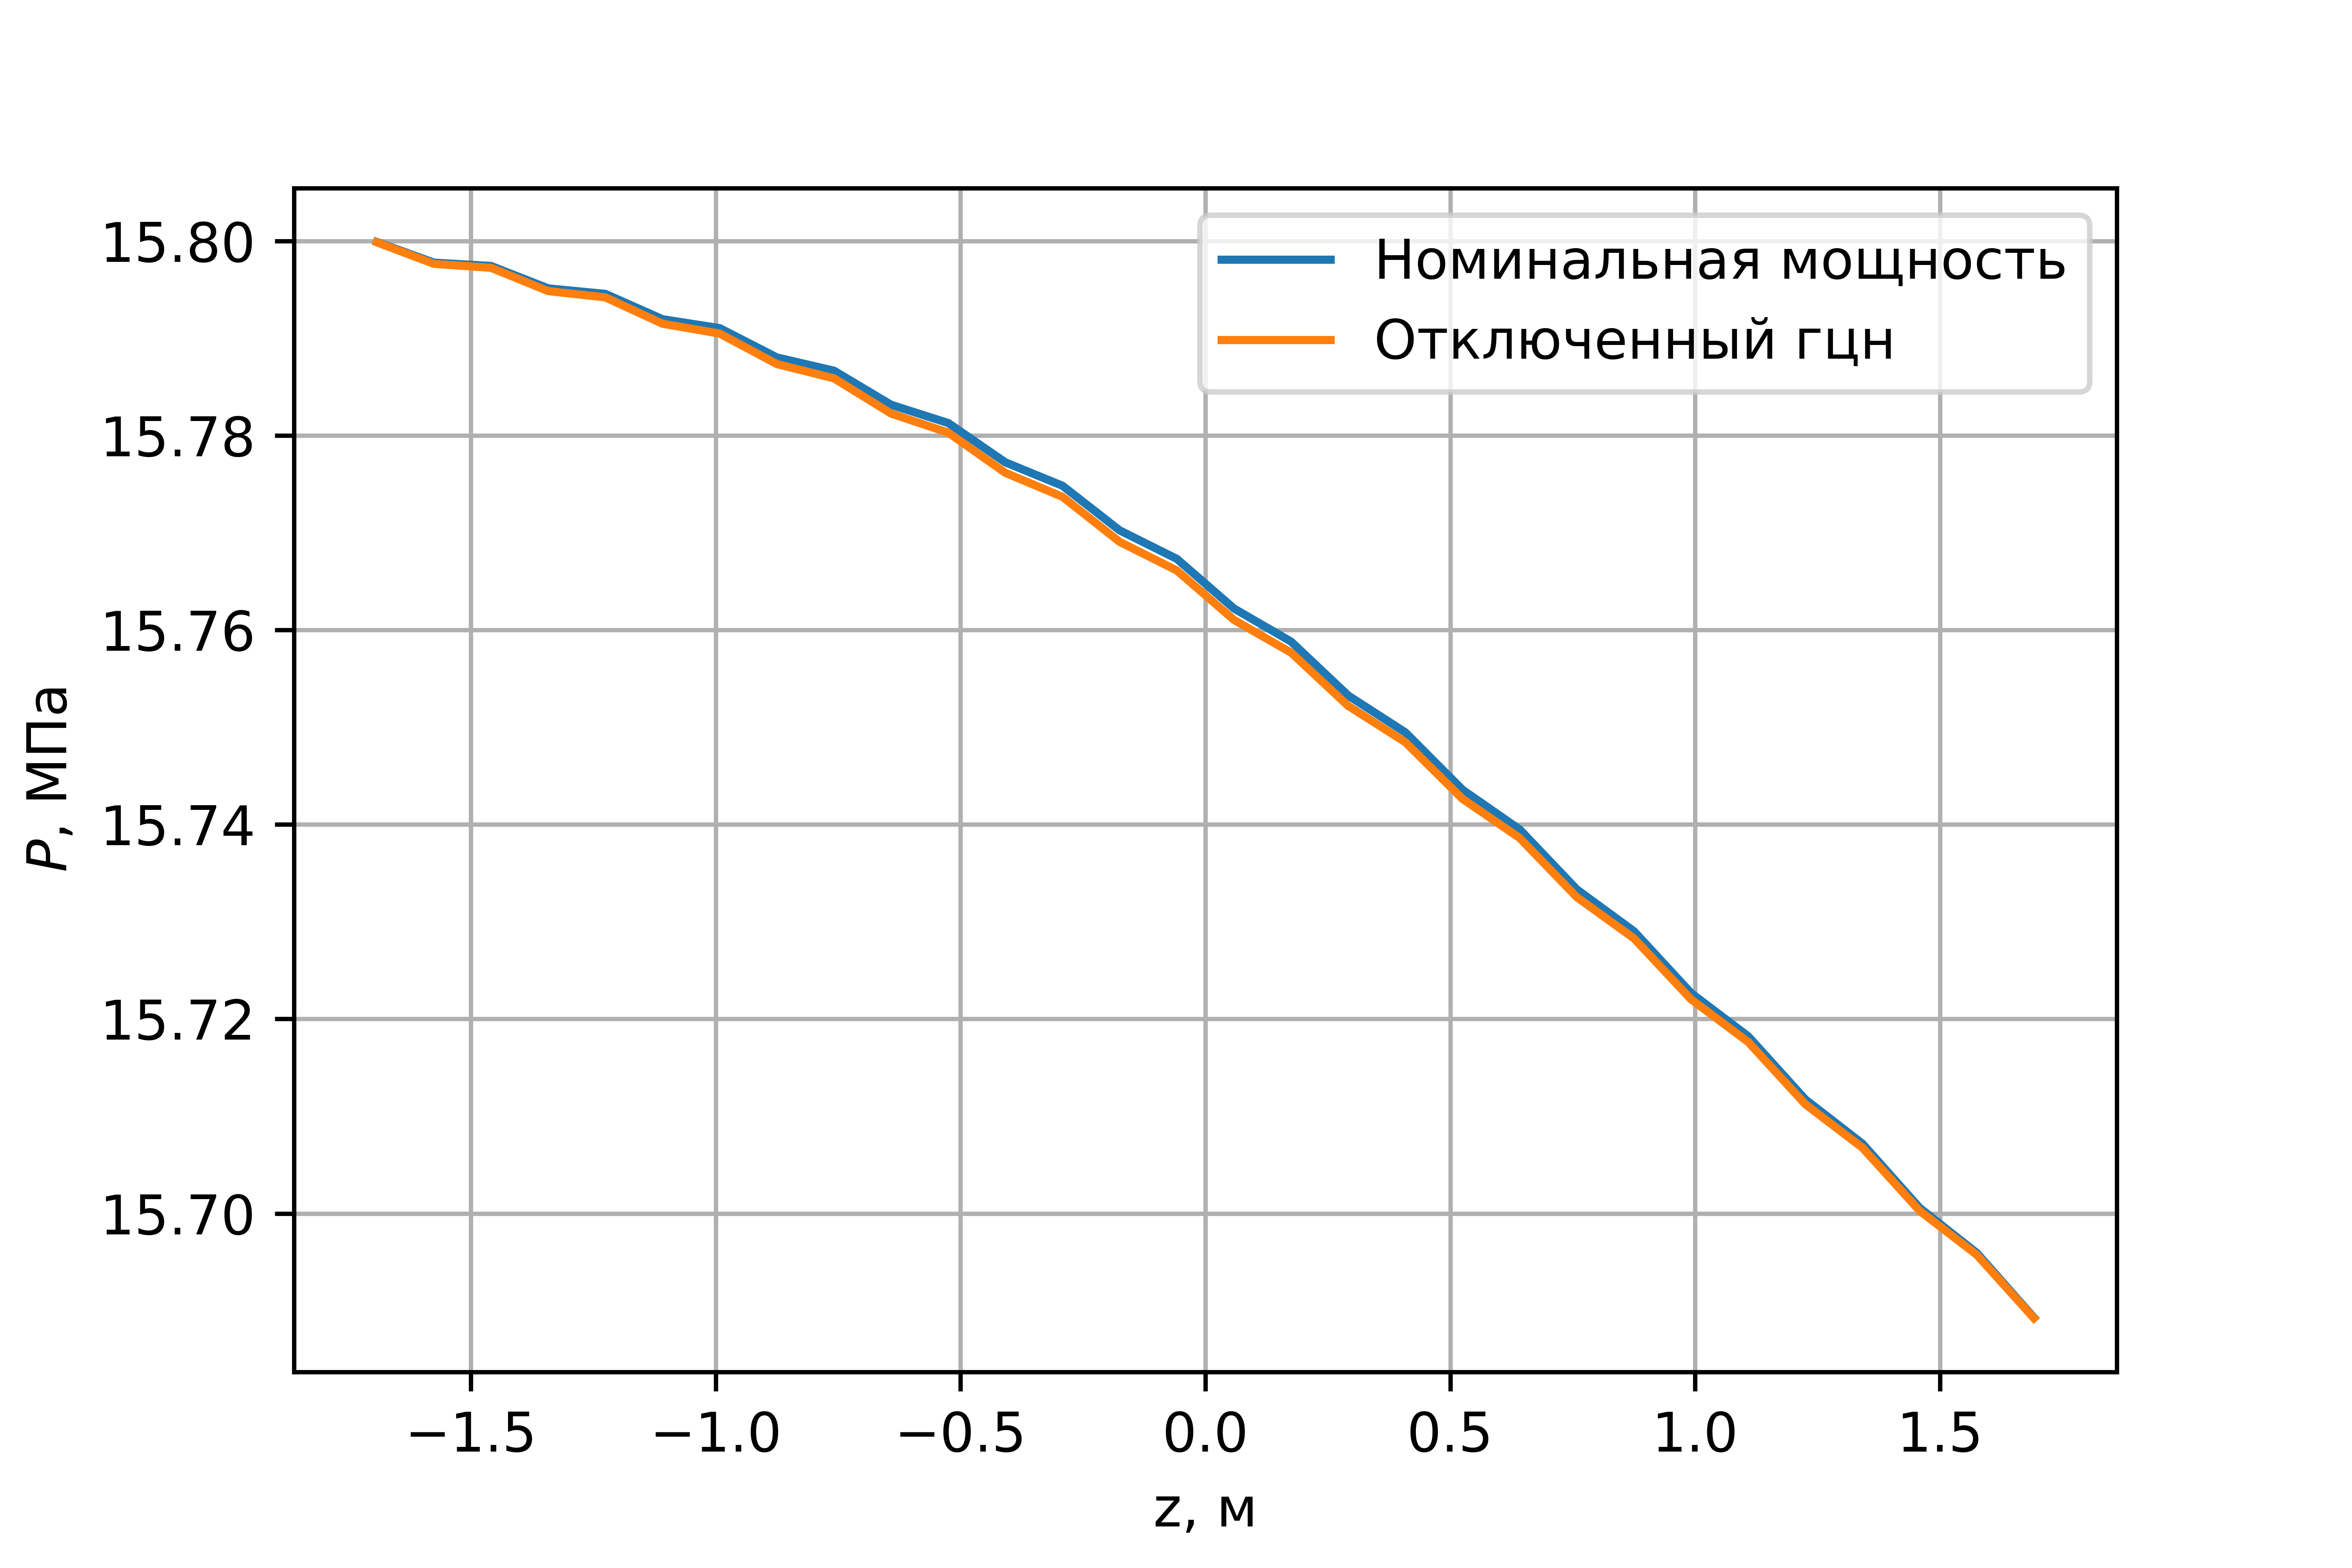
\includegraphics{p_one_gcn_max.png}
% 		\caption{распределение давления в центральной ТВС}
% 		\label{pic:p-one-gcn-max}
% 	\end{center}
% \end{figure}

\subsection{Расчет теплогидравлических характеристик при отлкючении двух ГЦН}
Аналогично проведенному расчету характеристик РУ при отключении одного ГЦН также был проведен расчет в случае отключения двух ГЦН, стоящих друг на против друга.

В расчетной модели была пониженная температура на входе до  $T_{\text{in}}^{\text{low}}=284 \circ C$ для двух петель. Температура была снижена для ячеек, расположенных в левой верхней и правой нижней области по картограмме \ref{pic:treton-quarts} при задании во входном файле T\_IN.TXT расчетного модуля «ТРЕТОН». В файл Q6.TXT входное тепловыделение для всех ячеек было снижено до 50\%$Q_{\text{ном}}$. 

По результатам расчета получены максимальные значения температур топлива, оболочек и теплоносителя, которые представлены в таблице \ref{tabular:t-two-gcn-nominal-compare}

\begin{table}[H]
    \caption{Максимальные температуры теплоносителя, топлива и оболочки твэлов при работе РУ на номинальной и повышенной мощности}
    \begin{center}
        \begin{tabular}{|l|c|c|}
        \toprule
        Тепловая мощность, МВт & 2903 & 1452 \\
        \midrule
        \hline
        Максимальная температура теплоносителя, $\circ C$ & 332.5 & 320.5  \\ 
        \hline
        Запас до кипения теплоносителя, $\circ C$ & 13.9 & 26 \\
        \hline
        Максимальная температура топлива, $\circ C$ & 1452 & 1067.8  \\
        \hline
        Максимальная температура внешней оболочки & 346.46 & 330 \\
        \hline
        Максимальная температура внутренней оболочки & 381.3 & 351.3 \\
        \hline
        Запас до кипения теплоносителя вблизи оболоки & 0.04 & 16.5 \\
        \bottomrule
        \end{tabular}
		\label{tabular:t-two-gcn-nominal-compare}
    \end{center}
\end{table}

\begin{figure}[H]
	\begin{center}
		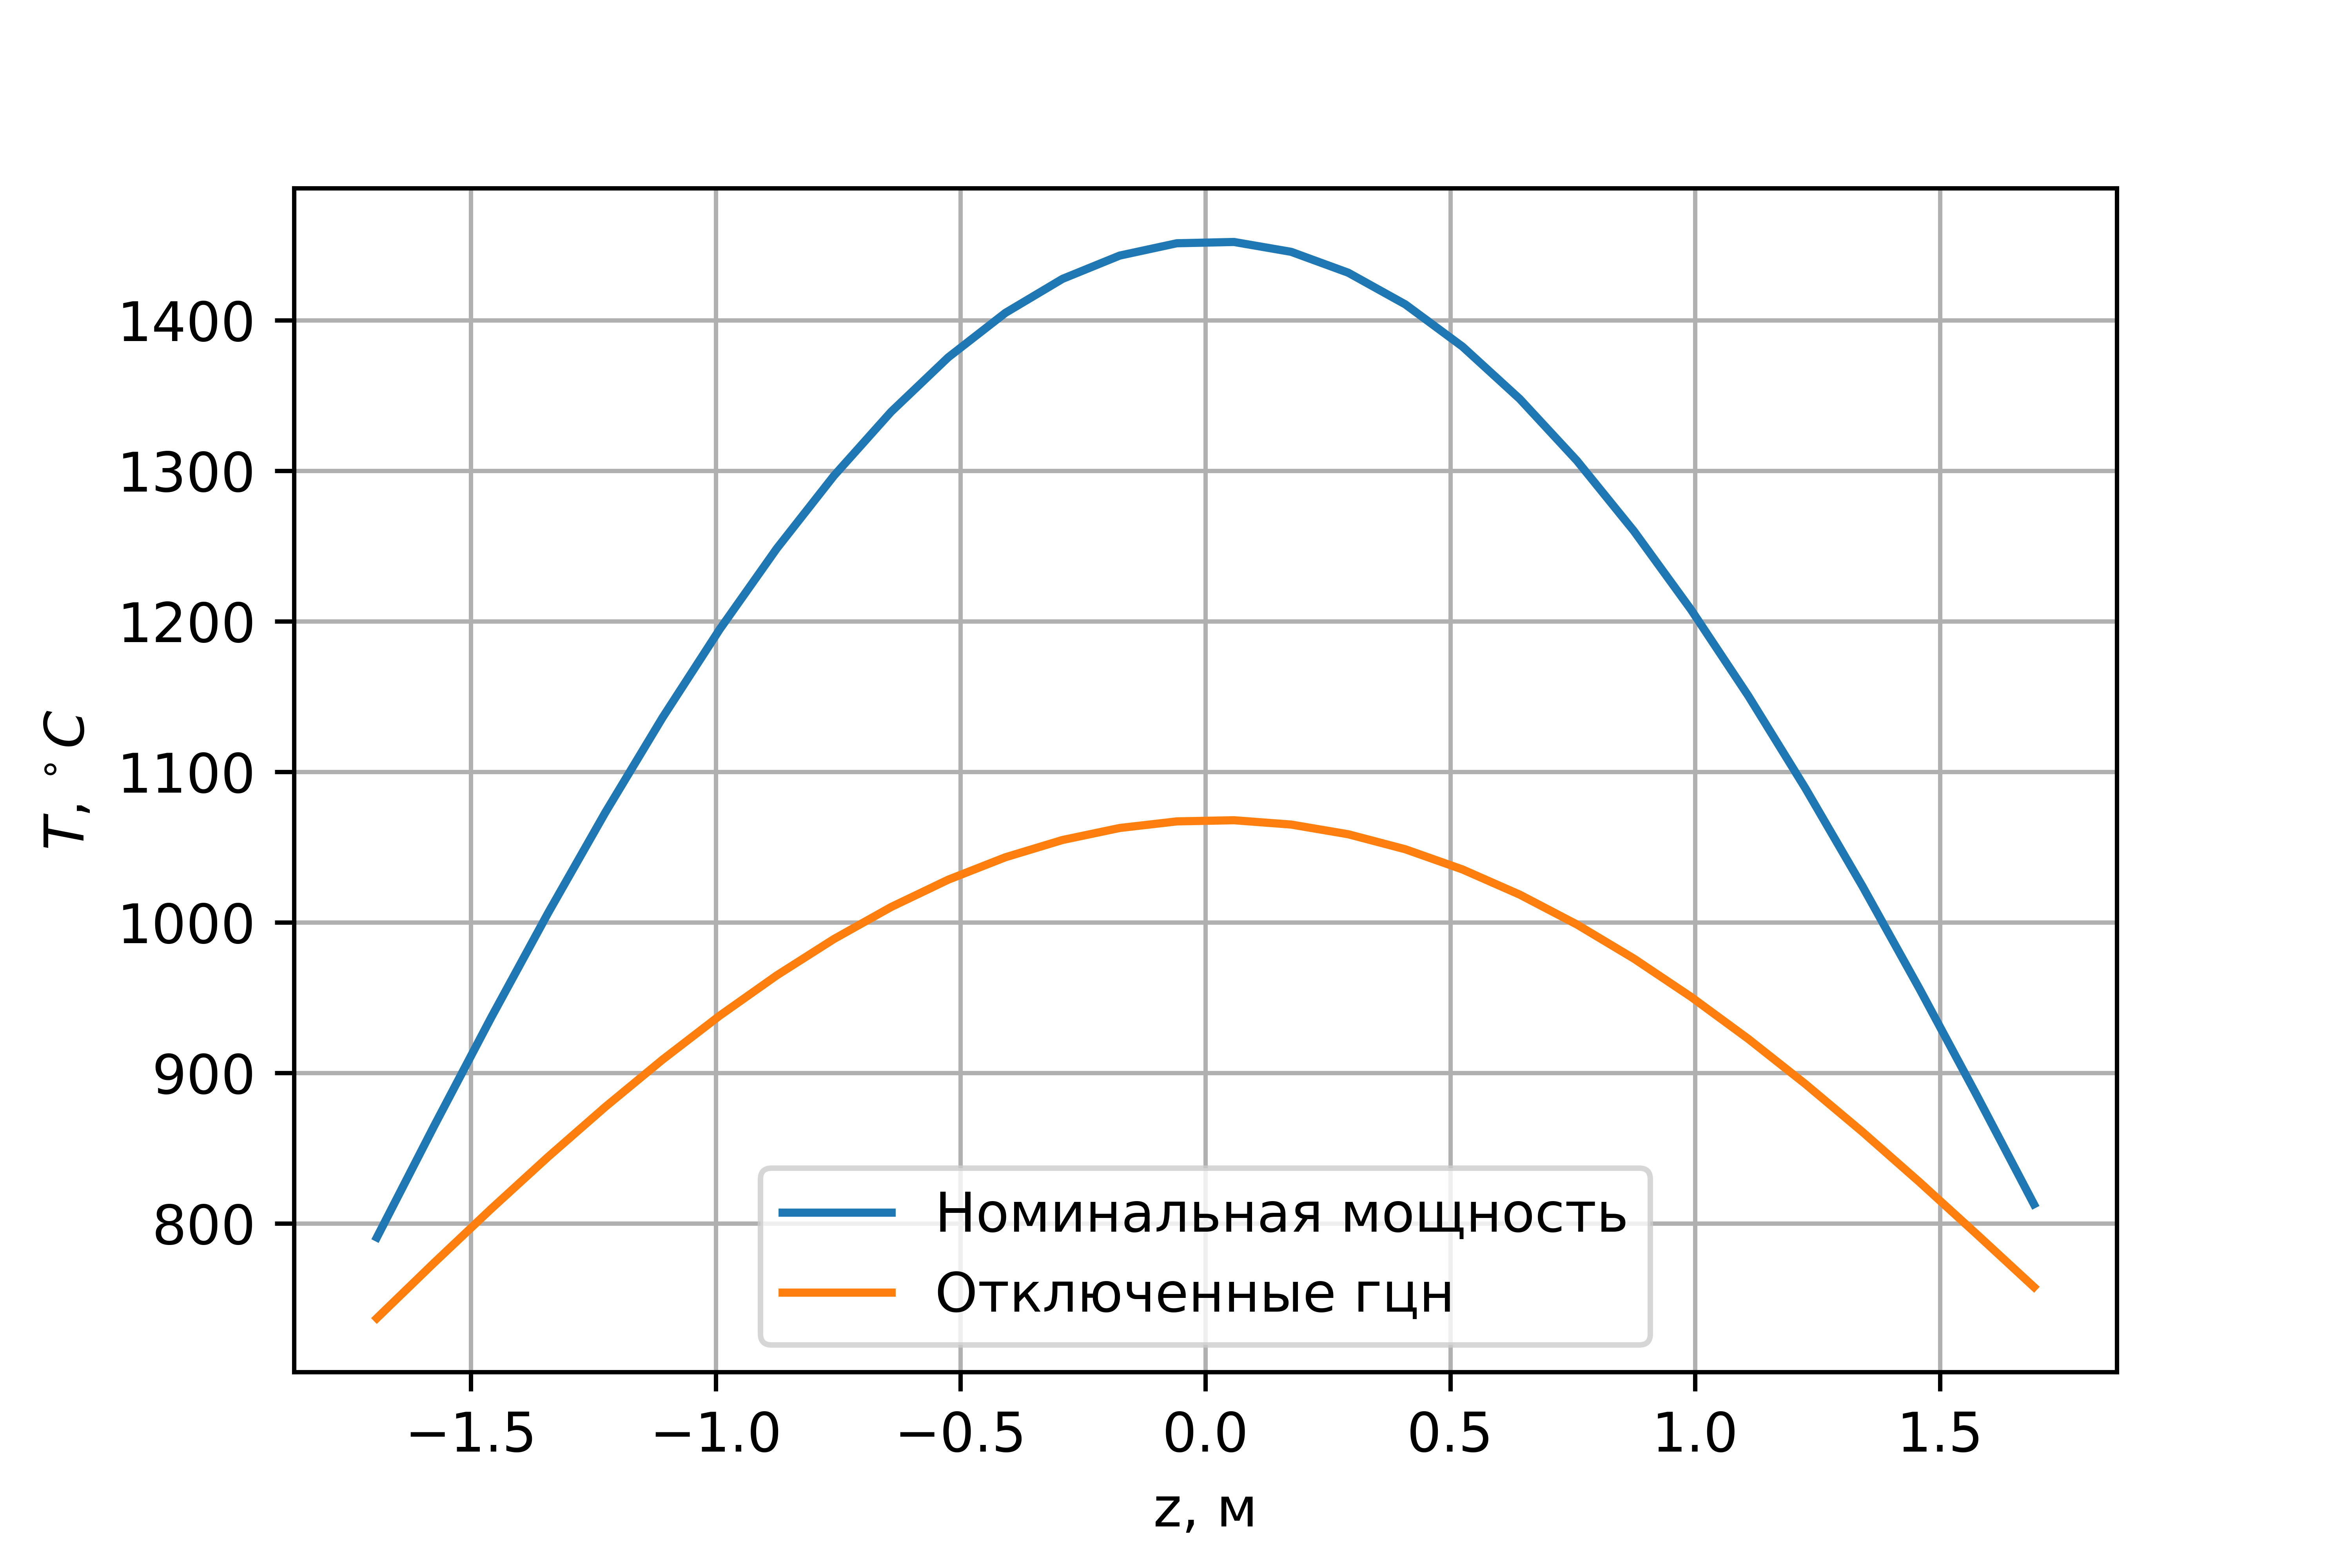
\includegraphics{treton_t_fuel_two_gcn_compare.png}
		\caption{Распределение температуры топлива по высоте АЗ}
		\label{pic:treton-t-fuel-two-gcn-compare}
	\end{center}
\end{figure}

\begin{figure}[H]
	\begin{center}
		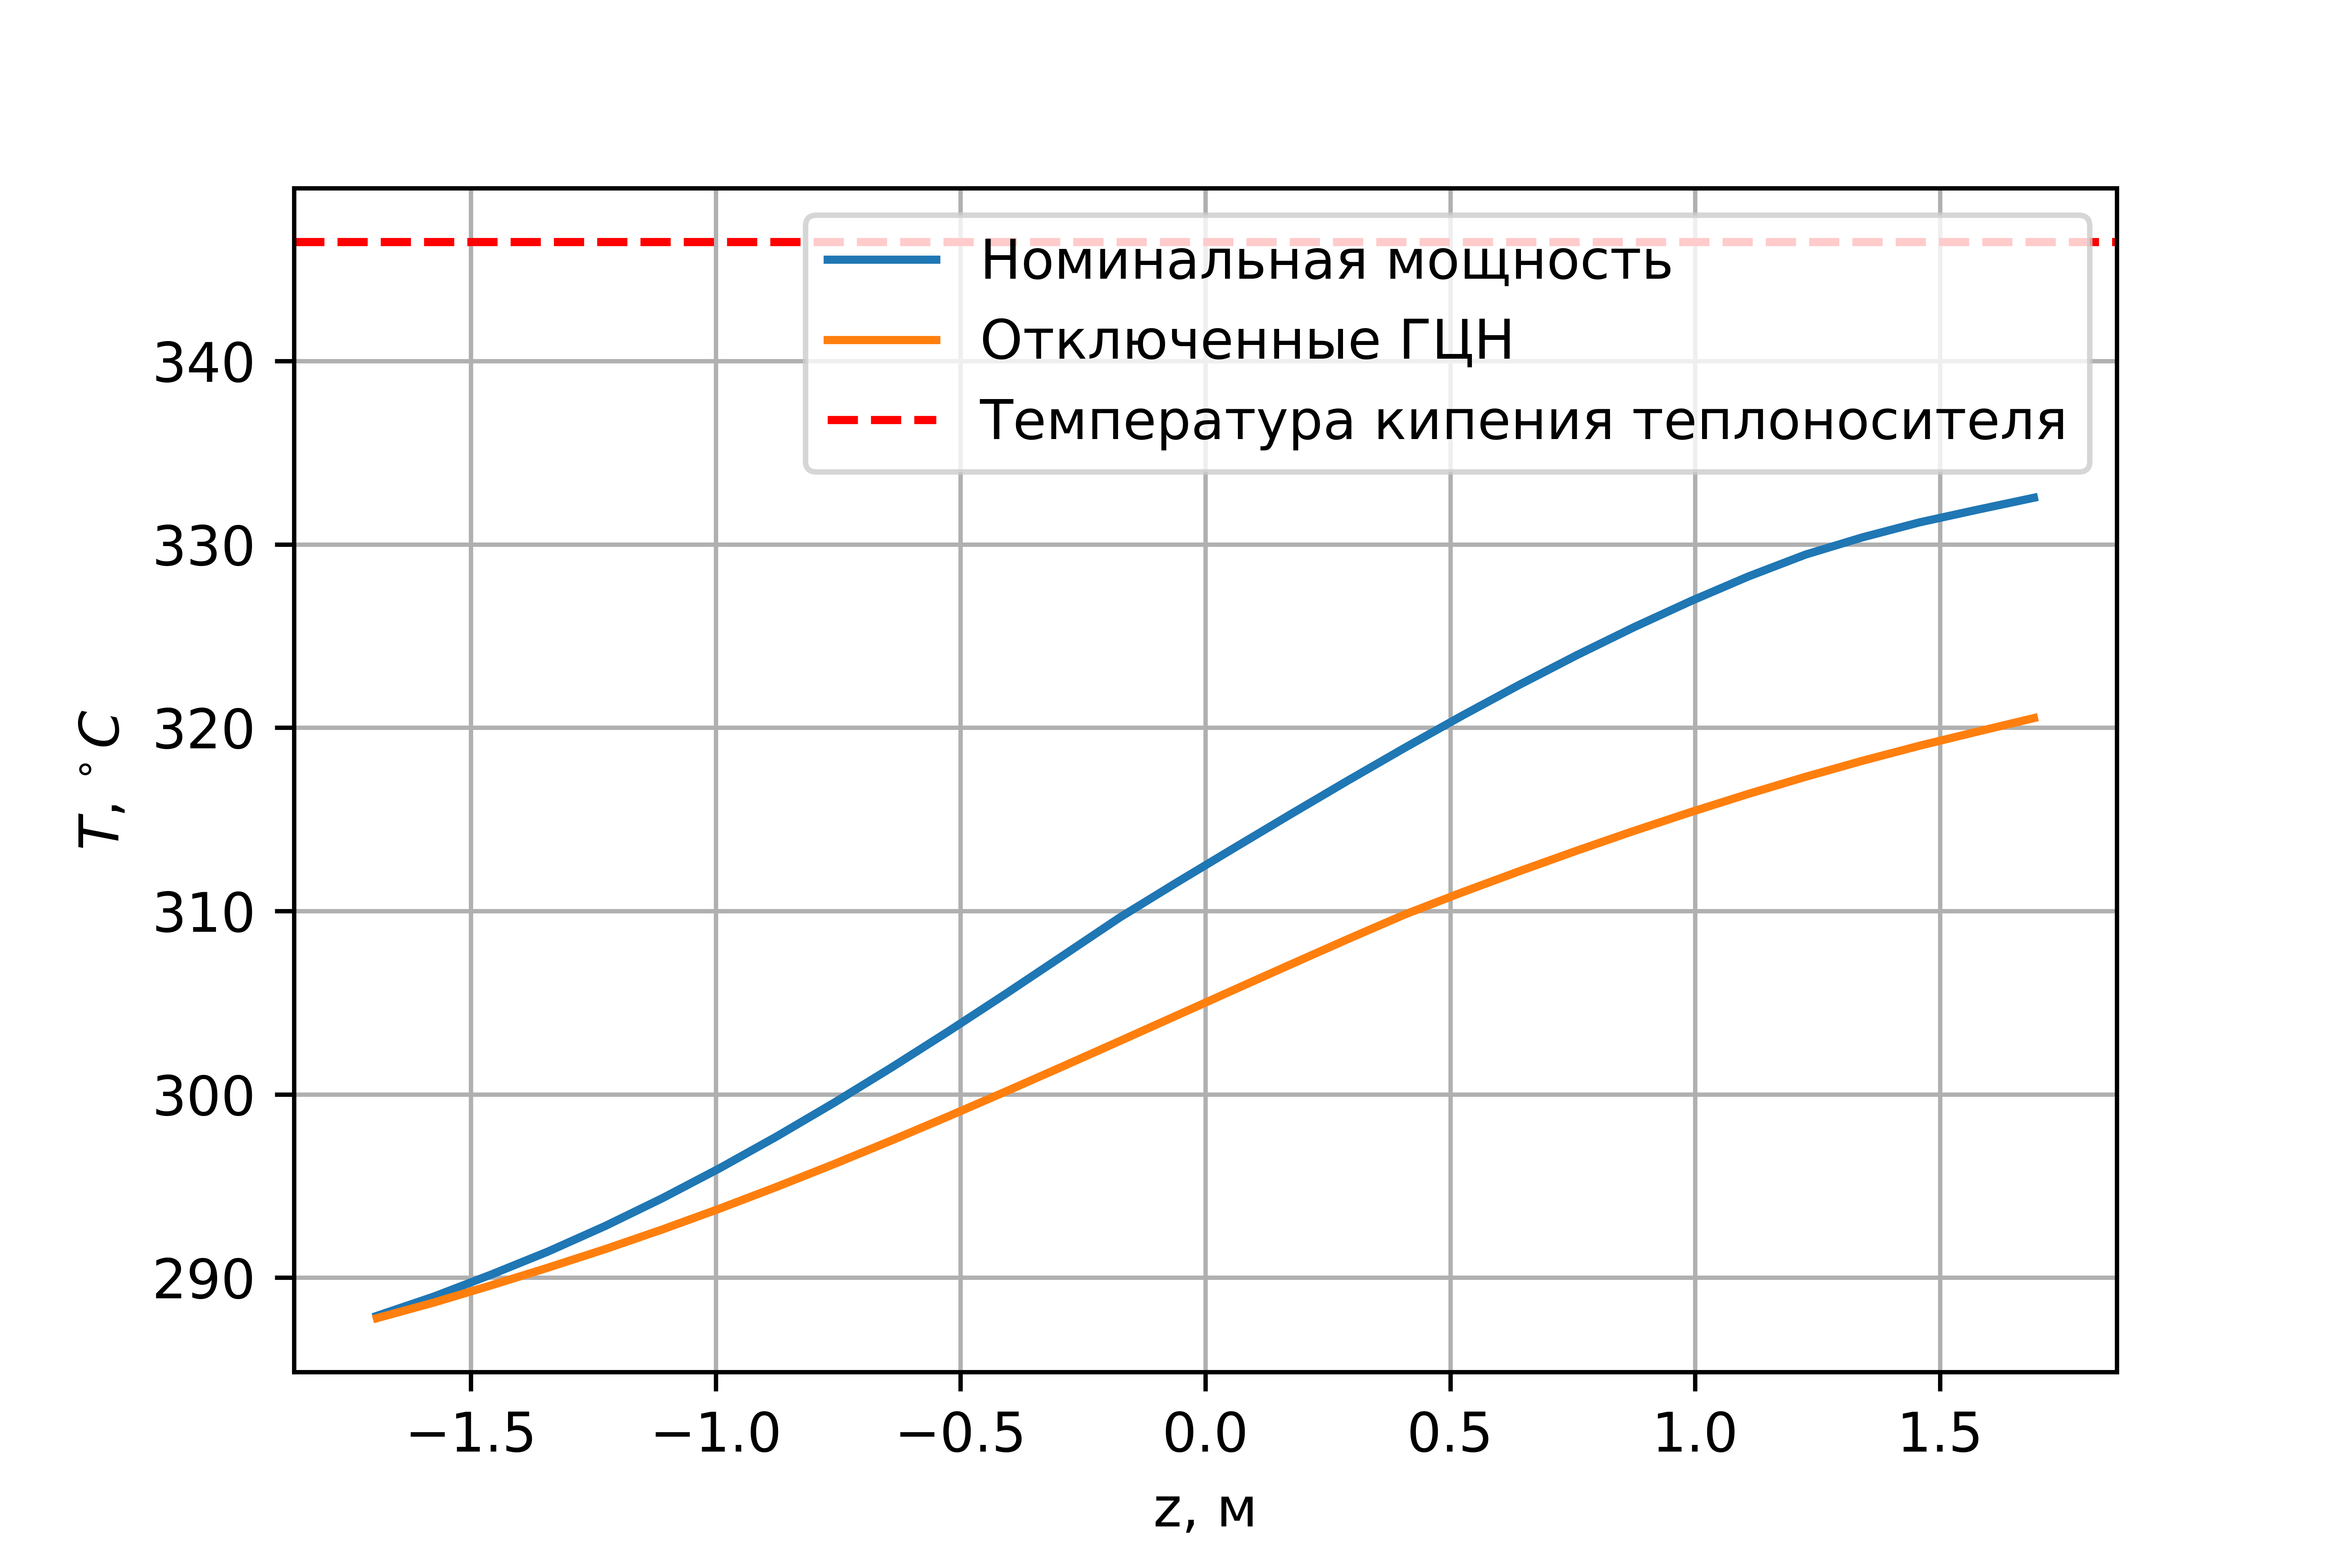
\includegraphics{treton_t_tepl_two_gcn_compare.png}
		\caption{Распределение температуры теплоносителя по высоте АЗ}
		\label{pic:treton-t-tepl-two-gcn-compare}
	\end{center}
\end{figure}

\begin{figure}[H]
	\begin{center}
		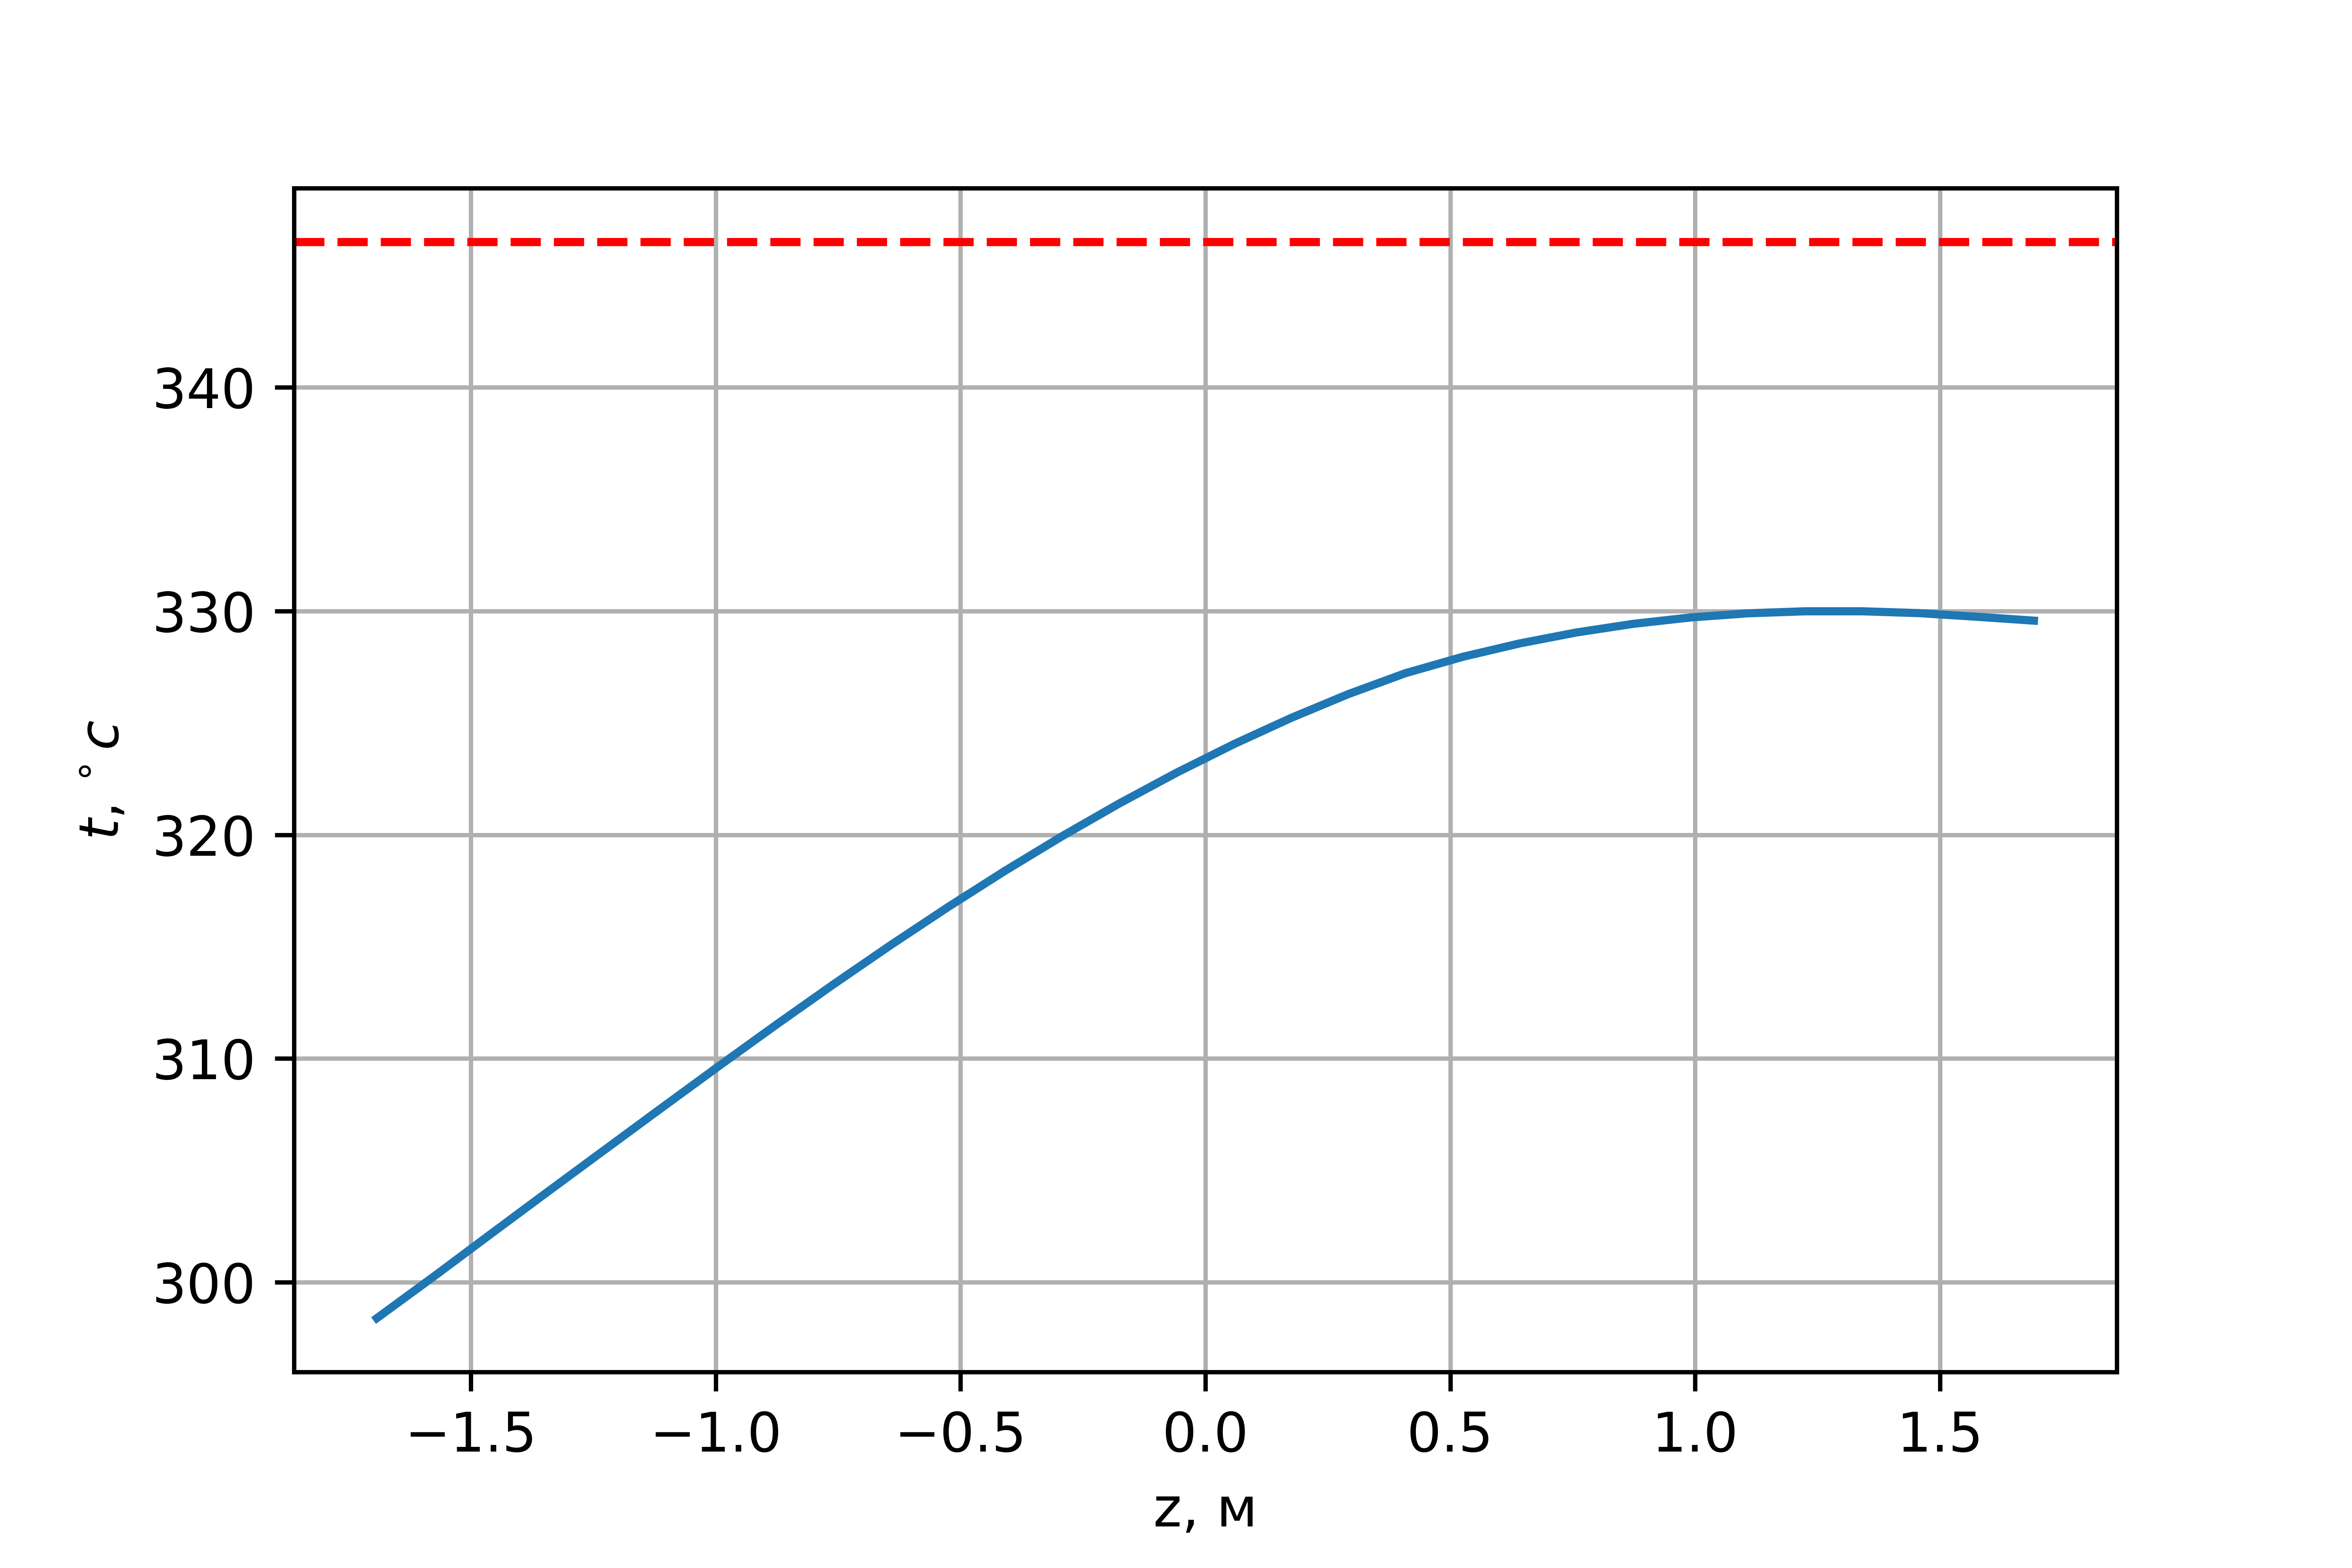
\includegraphics{treton_two_gcn_obl_naruj_max.png}
		\caption{Распределение температуры наруженй оболочки твэлов по высоте для кассеты с максимальной температурой теплоносителя}
		\label{pic:treton-two-gcn-obl-naruj-max}
	\end{center}
\end{figure}

Общий график температур для работы реактора при работе на пониженной мощности в следствие отключения двух ГЦН представлен на рисунке \ref{pic:treton-two-gcn-obl-tepl-obsh}

\begin{figure}[H]
	\begin{center}
		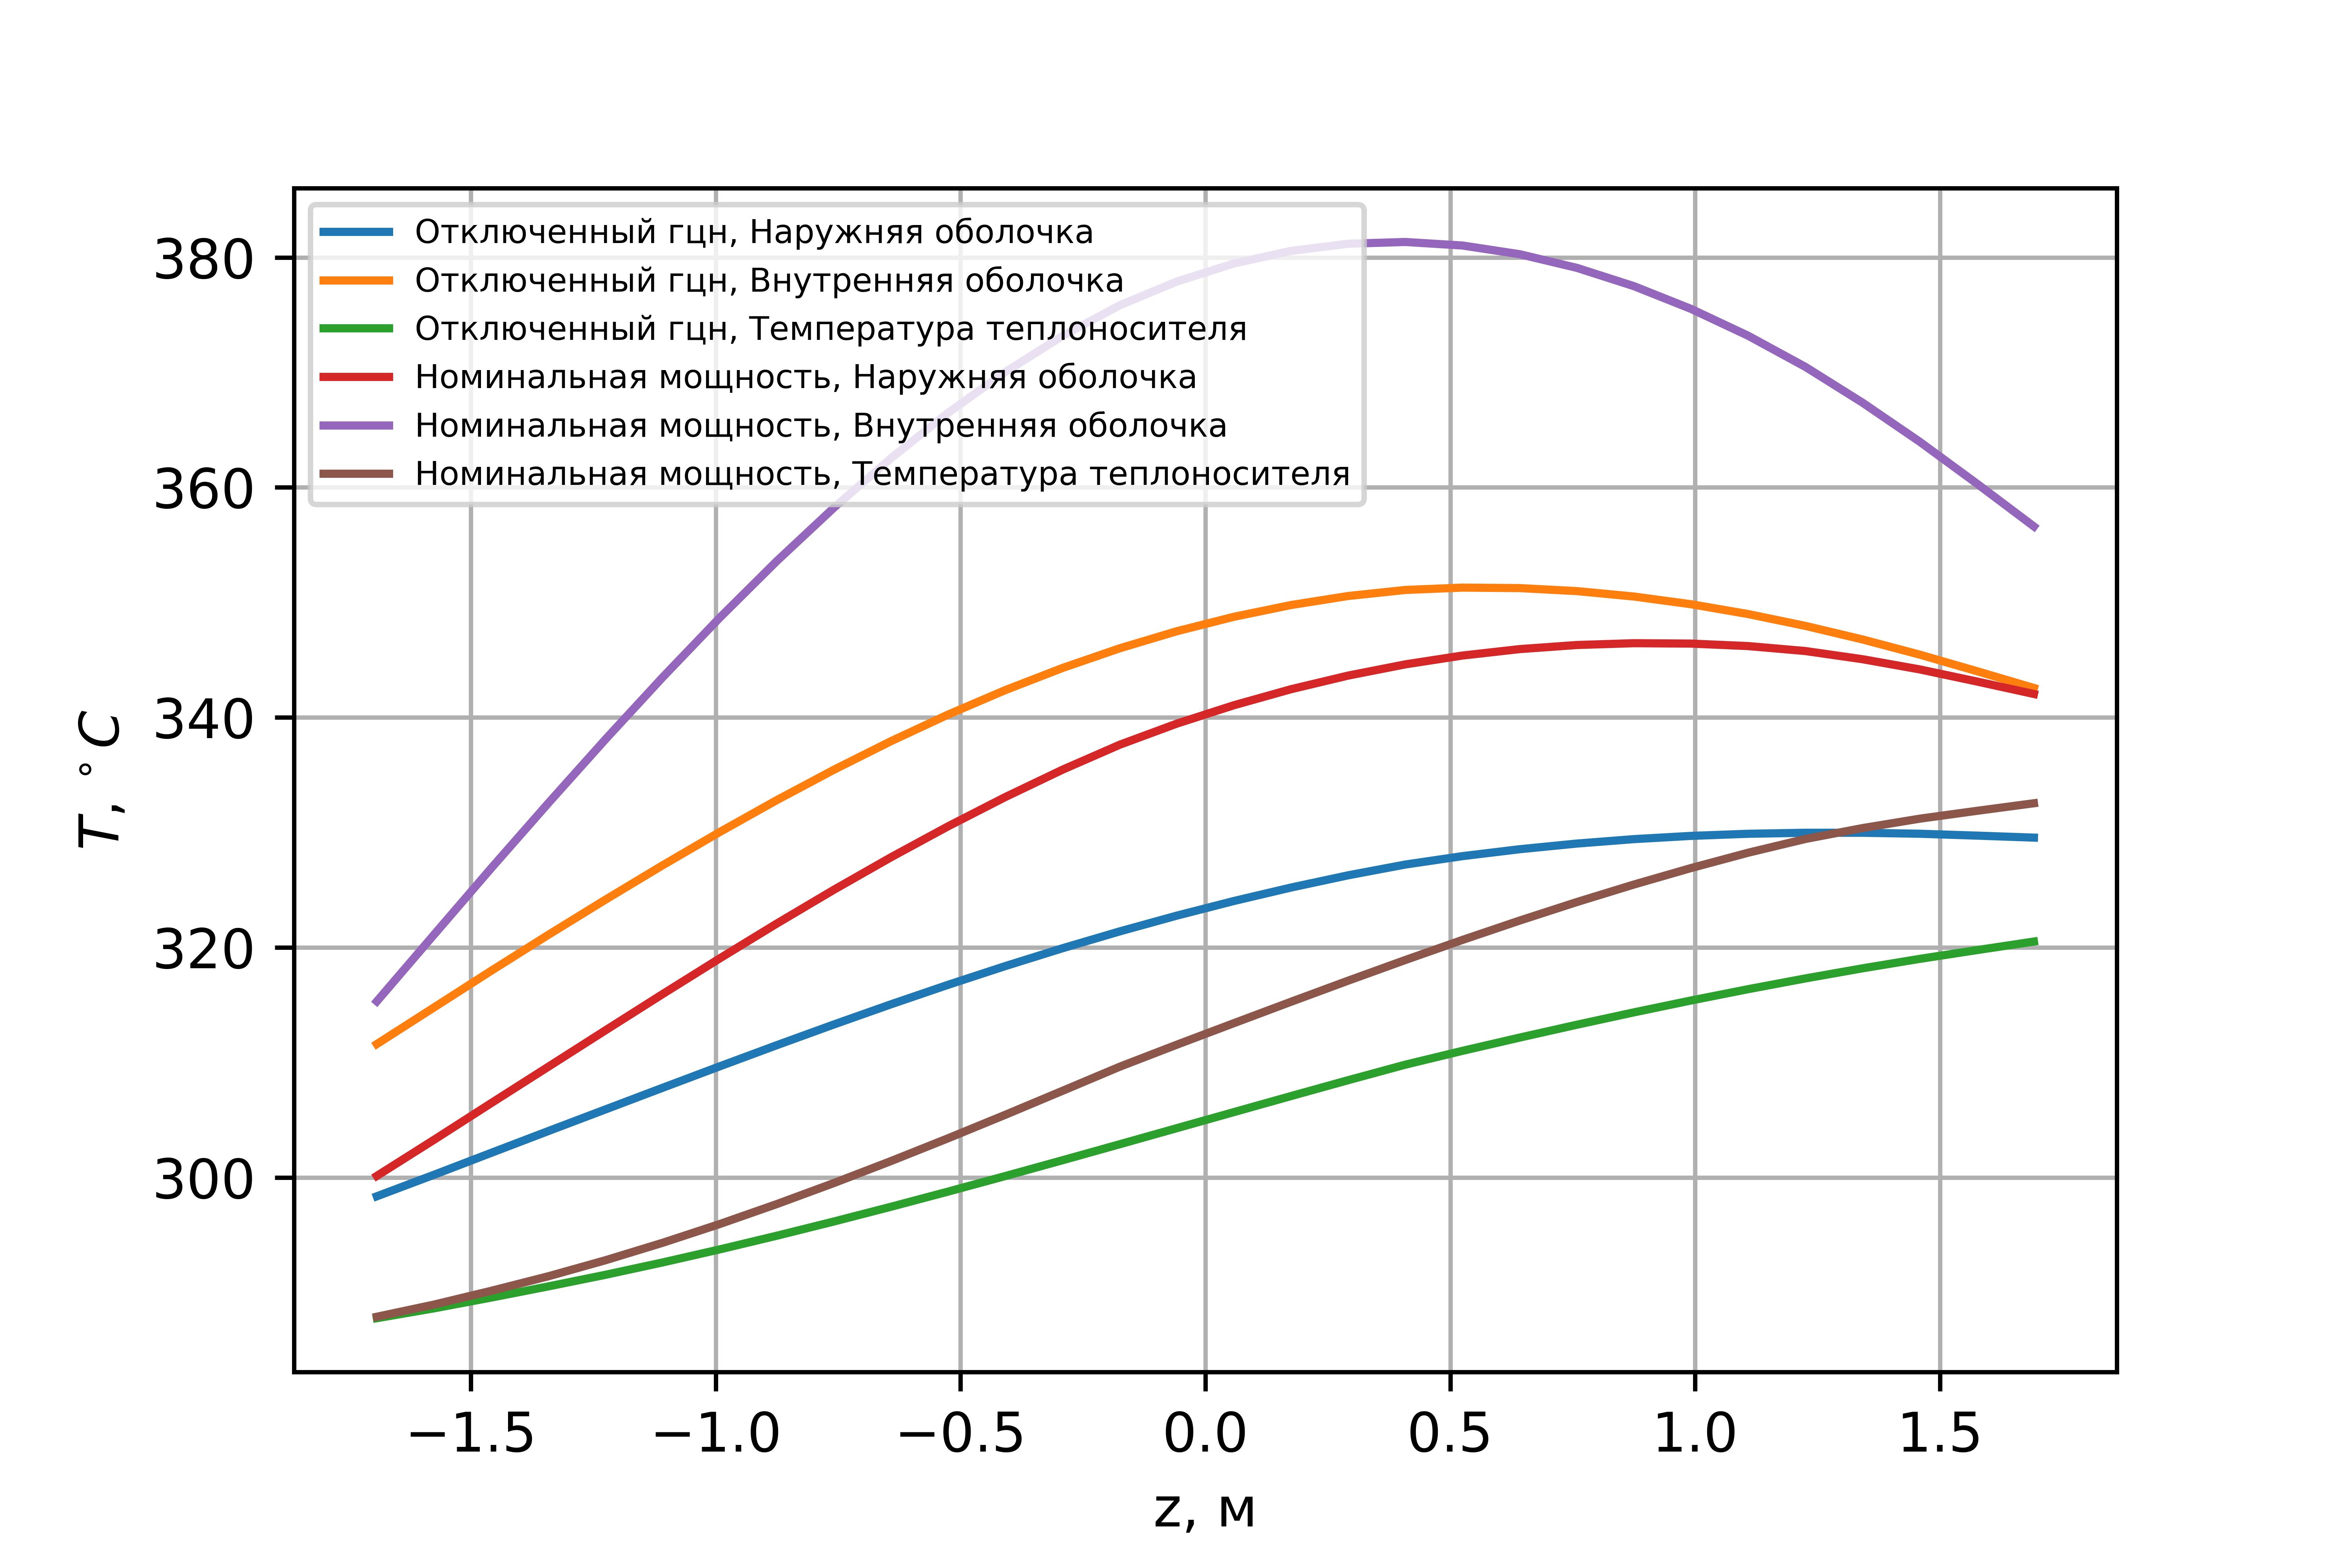
\includegraphics{treton_two_gcn_obl_tepl_obsh.png}
		\caption{Распределение температур по высоте АЗ}
		\label{pic:treton-two-gcn-obl-tepl-obsh} % название для ссылок внутри кода
	\end{center}
\end{figure}

На \ref{pic:podogrev-two-gcn} видно, что при отключении двух ГЦН подогрев в центральной ТВС уменьшился на 12 градусов, средний по всем ТВС подогрев уменьшился на 9.3. 

Для наблюдения возникающей при отключении неравномерности поля температур было построено распределение температуры теплоносителя на входе в активную зоны и на выходе из нее. Соответствующие зависимости представлены на \ref{pic:treton-two-gcn-t-all-cells-z-is-0}, \ref{pic:treton-two-gcn-t-all-cells-z-is-29}. Из графиков можно определить установившиеся две температурные зоны в реакторе, возникшие в слествие захолаживания теплоносителя в петлях с отключенными ГЦН. Для оценки максимального эффекта от неравномерности энерговыделения было построено распределение температуры теплоносителя по высоте АЗ для второй радиальной группы, соответствующей семи ТВС вокруг центрального. Распределение представлено на рисунке \ref{pic:treton-two-gcn-2-radius-T}.

\begin{figure}[H]
	\begin{center}
		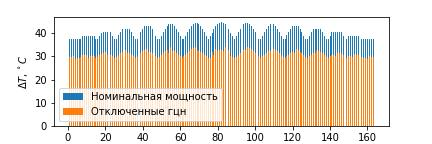
\includegraphics{podogrev_two_gcn.jpg}
		\caption{Распределение подогревов по всем ТВС}
		\label{pic:podogrev-two-gcn} % название для ссылок внутри кода
	\end{center}
\end{figure}

\begin{figure}[H]
	\begin{center}
		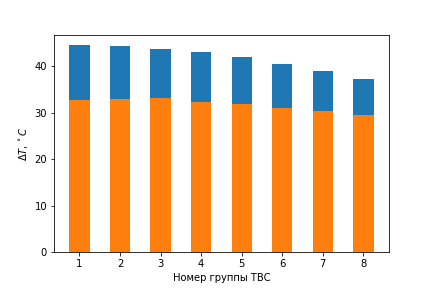
\includegraphics{podogrev_two_gcn_by_r.png}
		\caption{Распределение подогревов по радиальным группам ТВС}
		\label{pic:podogrev-two-gcn-by-r} % название для ссылок внутри кода
	\end{center}
\end{figure}

\begin{figure}[H]
	\begin{center}
		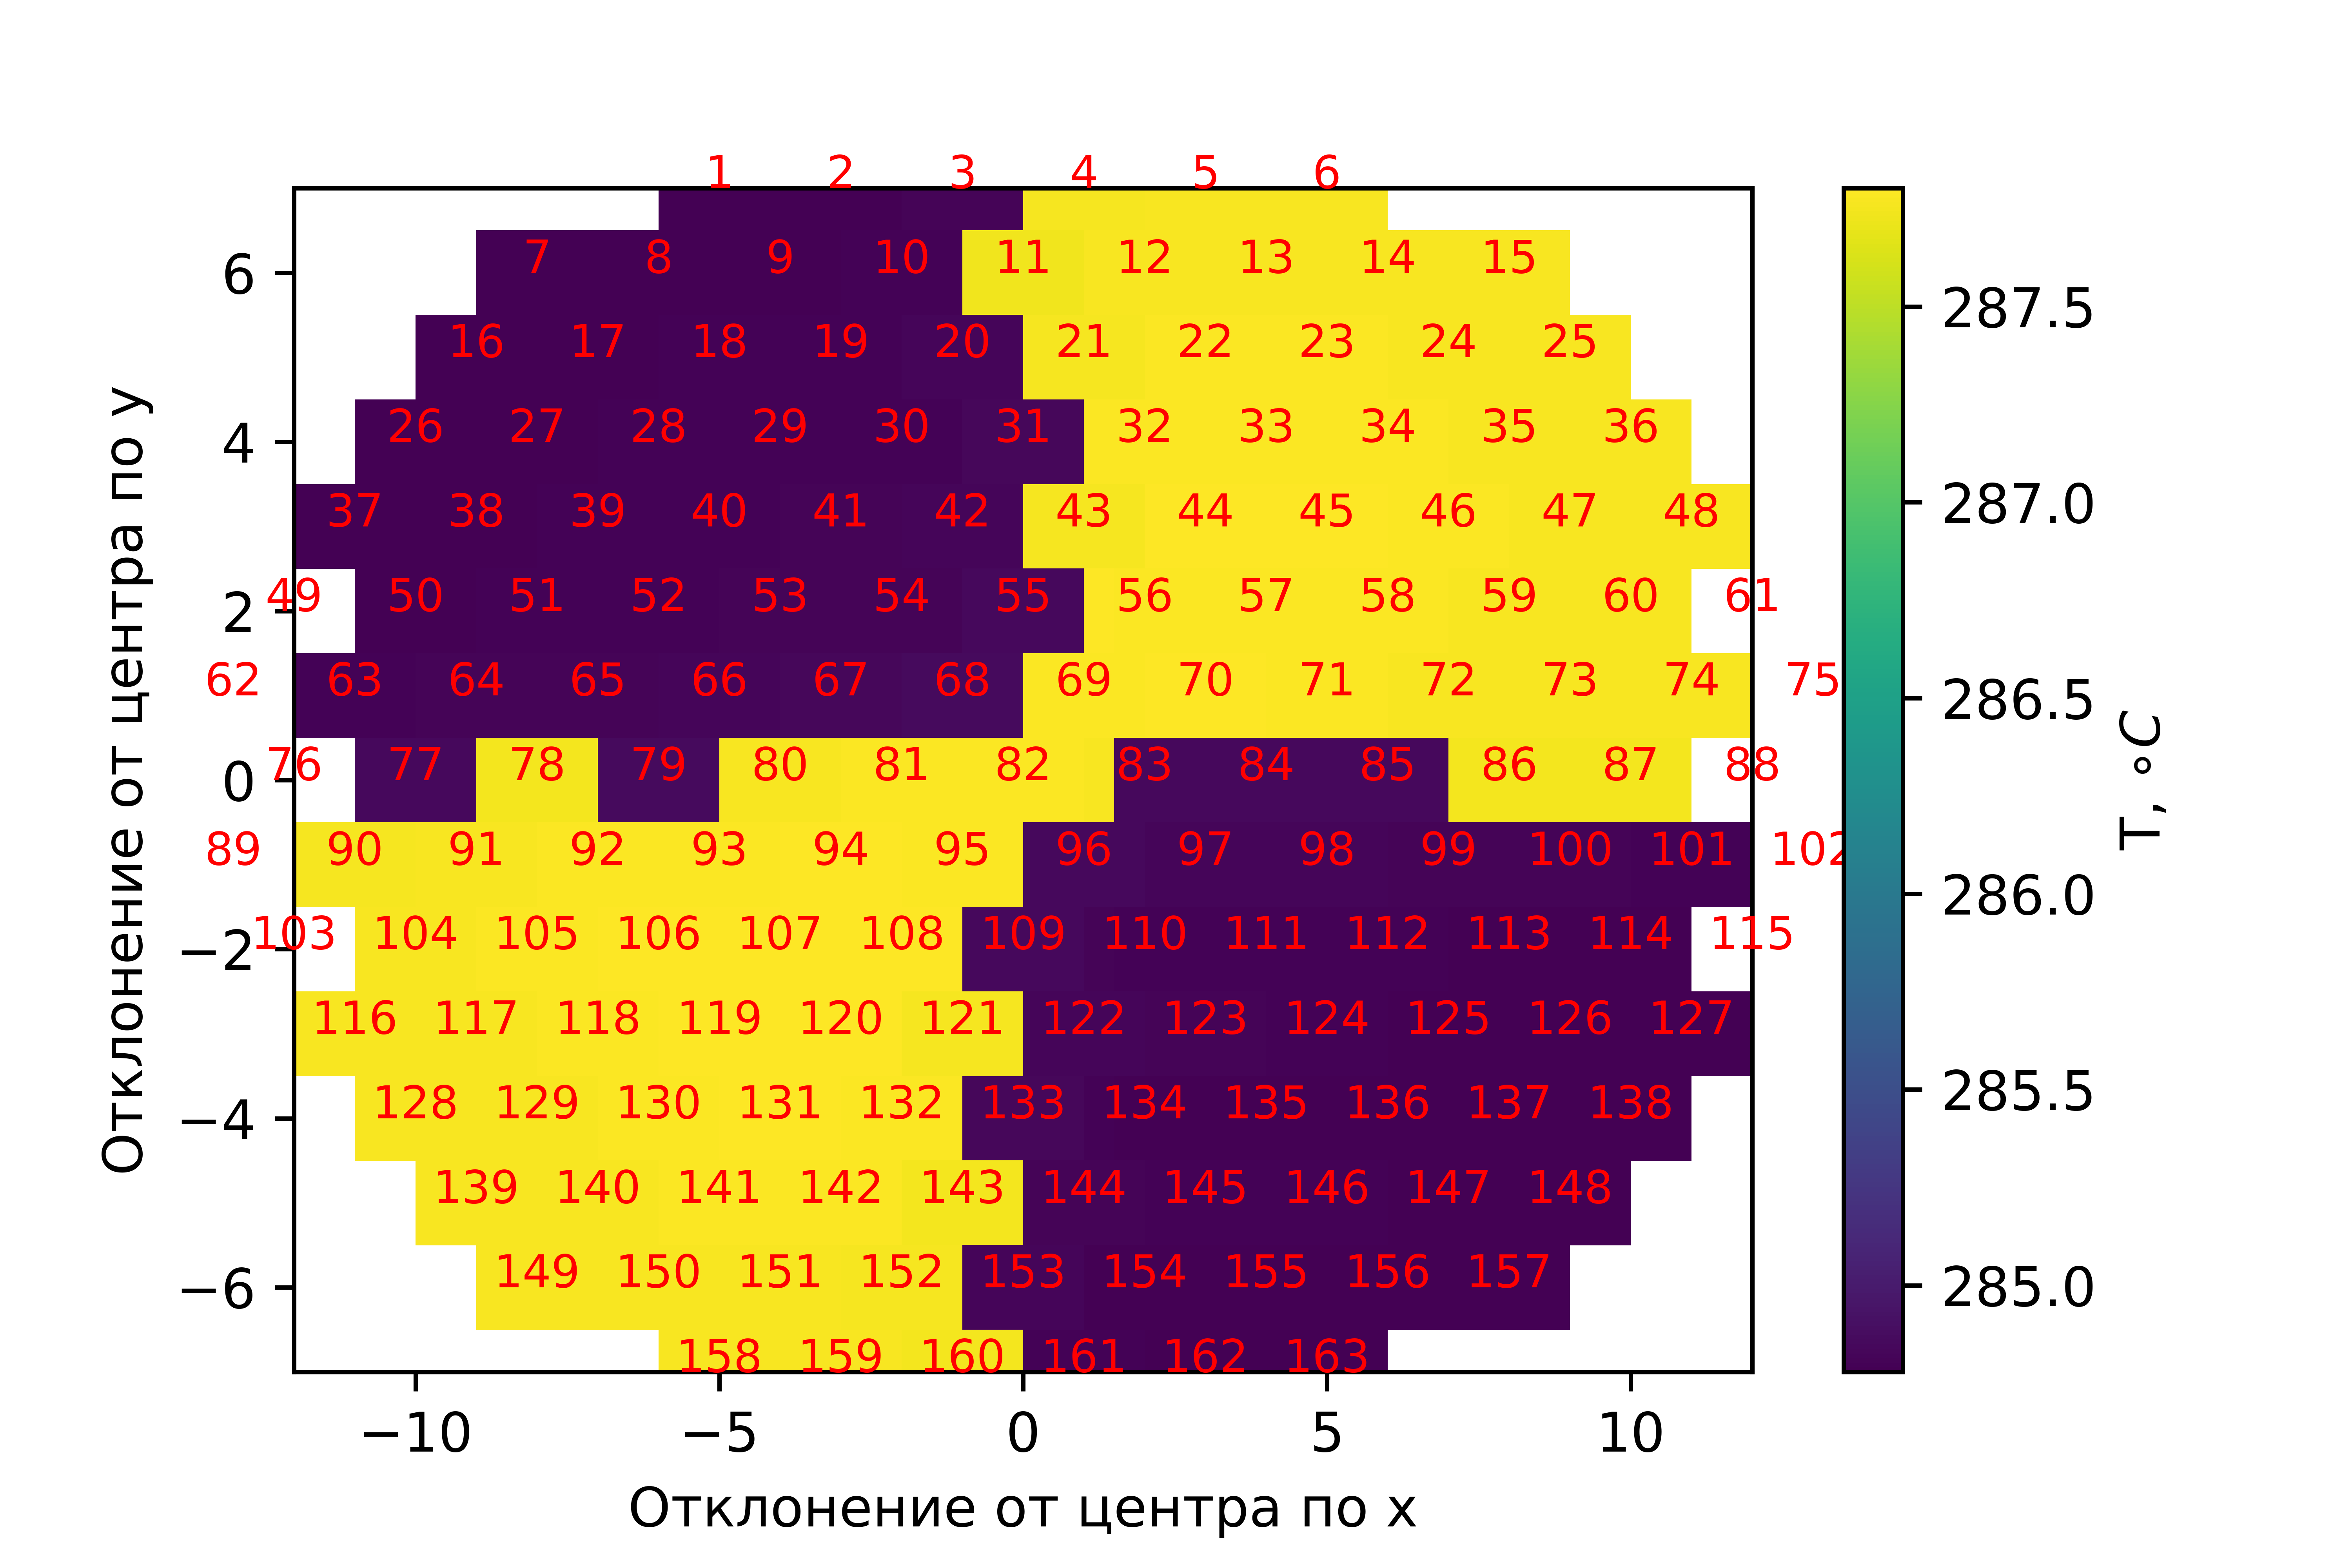
\includegraphics{treton_two_gcn_t_all_cells_z_is_0.png}
		\caption{Распределение температуры теплоносителя по ТВС на входе в АЗ}
		\label{pic:treton-two-gcn-t-all-cells-z-is-0} % название для ссылок внутри кода
	\end{center}
\end{figure}

\begin{figure}[H]
	\begin{center}
		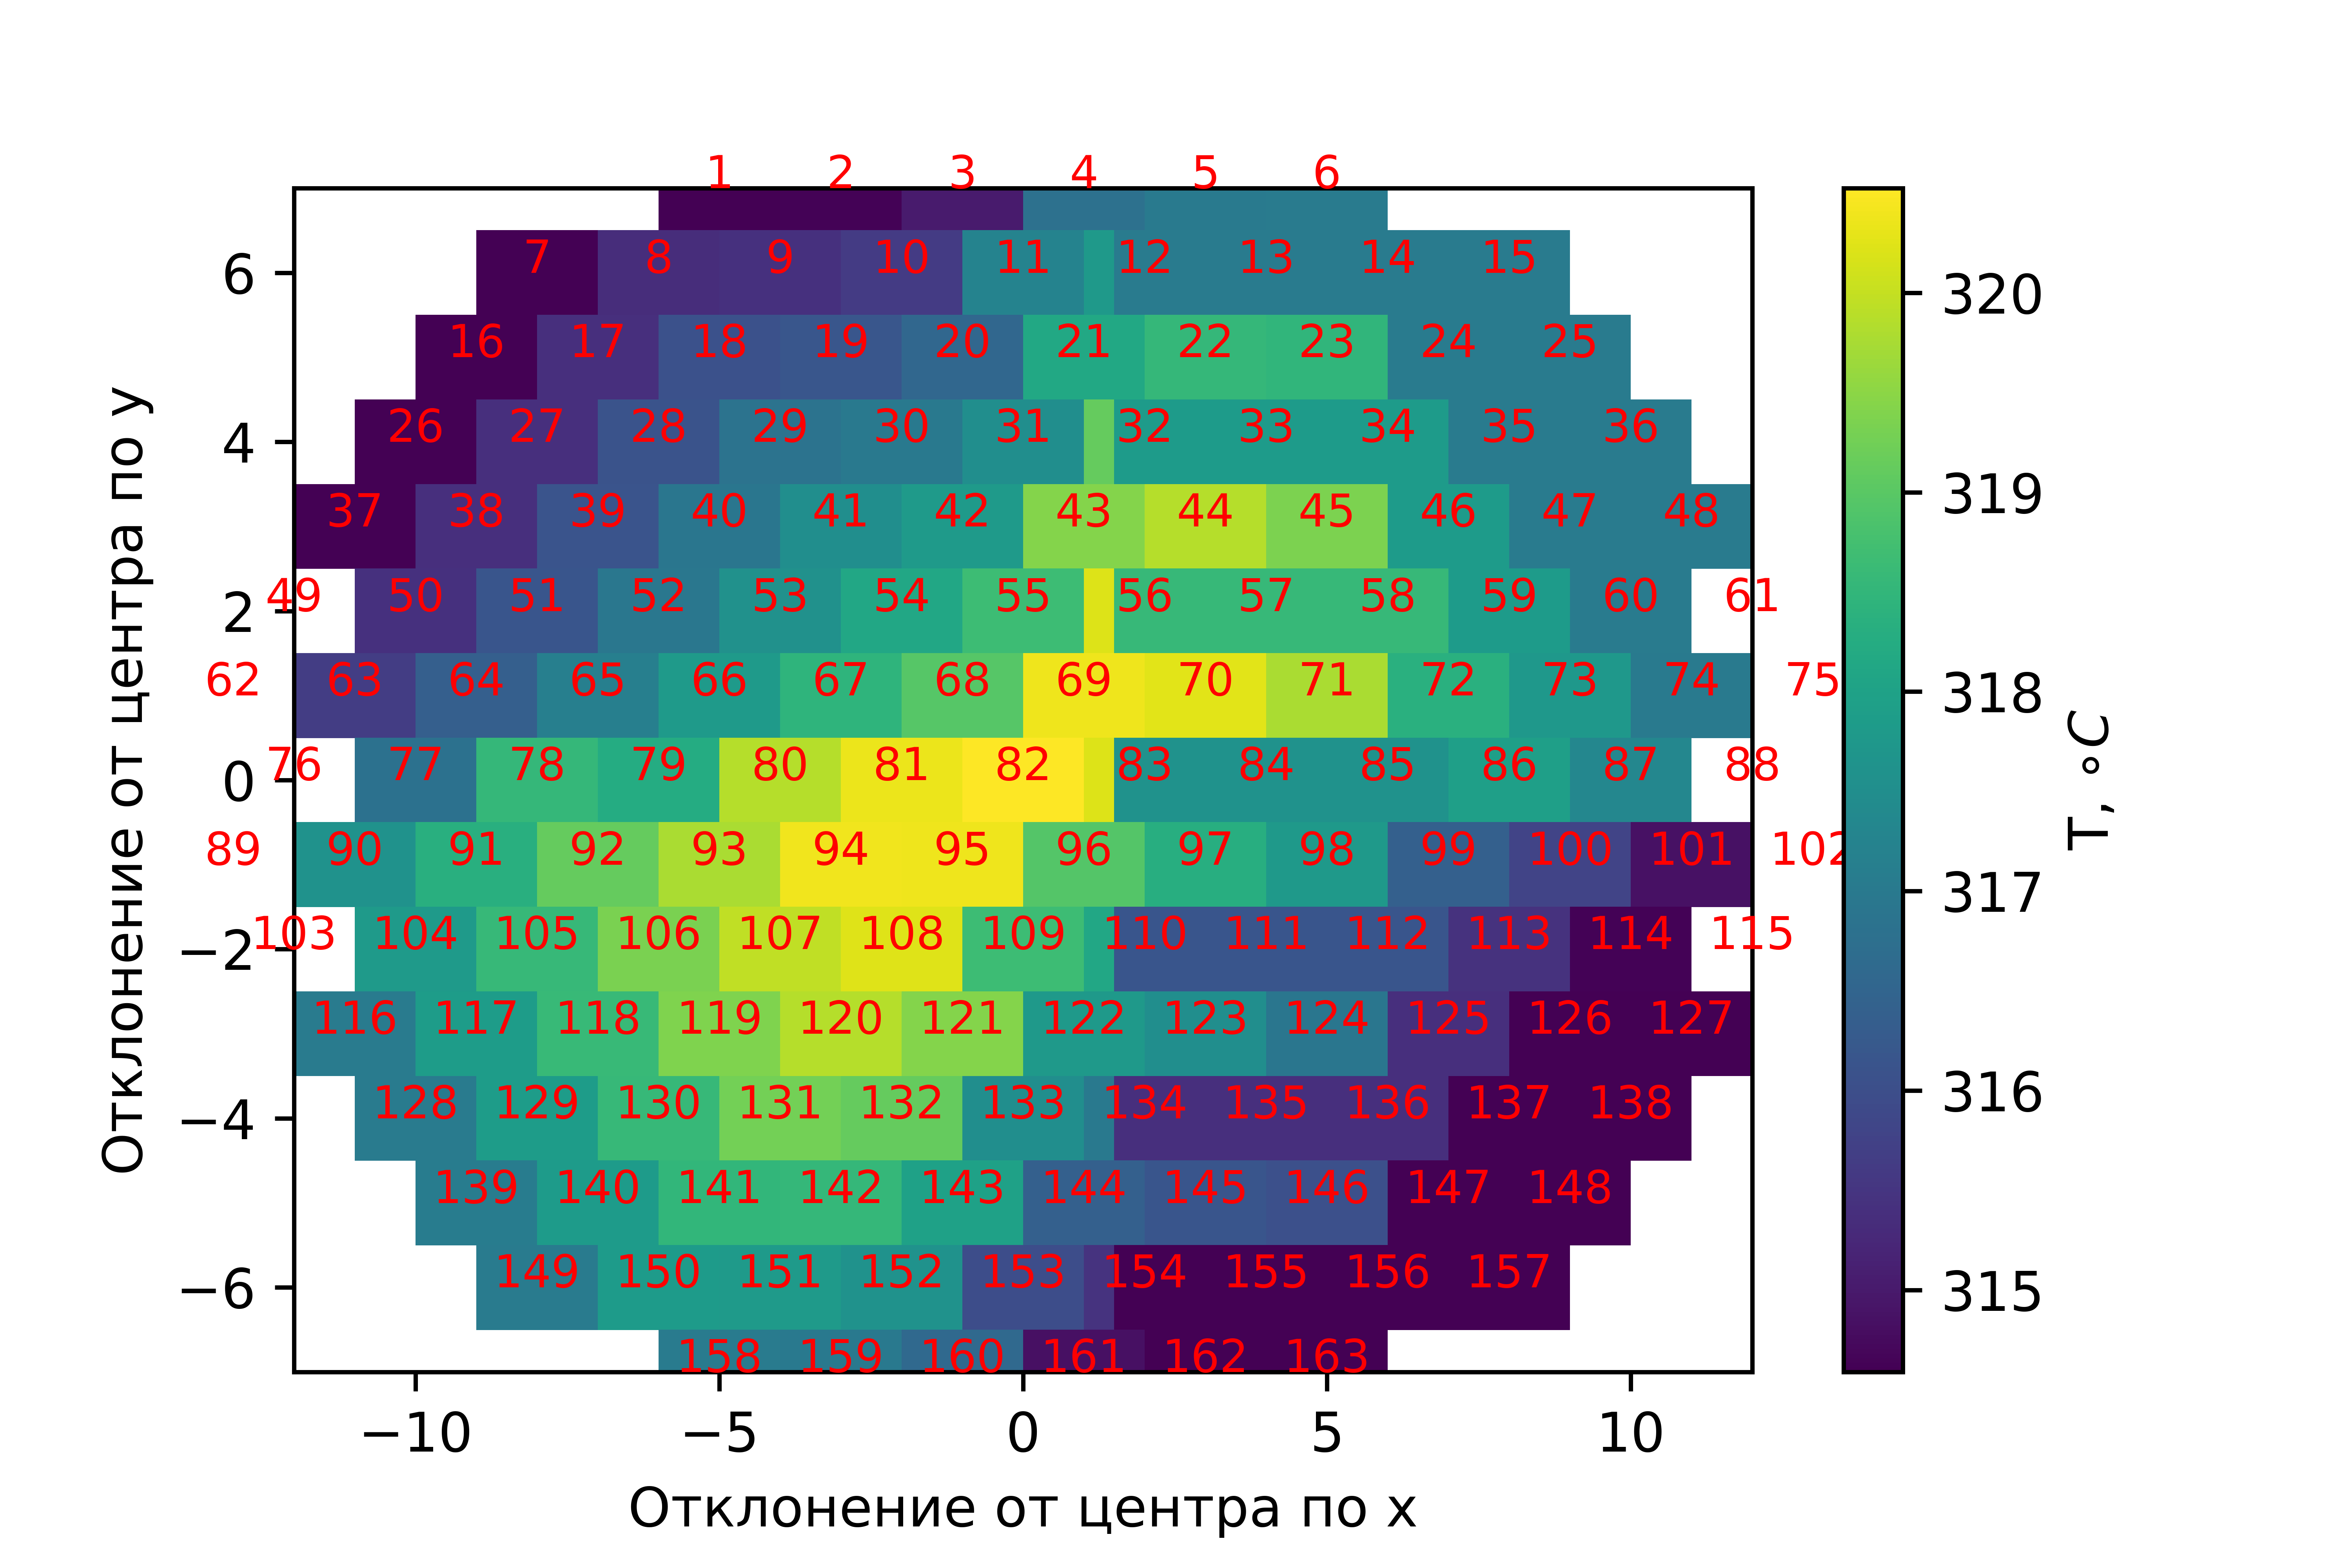
\includegraphics{treton_two_gcn_t_all_cells_z_is_29.png}
		\caption{Распределение температуры теплоносителя по ТВС на выходе из АЗ}
		\label{pic:treton-two-gcn-t-all-cells-z-is-29}
	\end{center}
\end{figure}


\begin{figure}[H]
	\begin{center}
		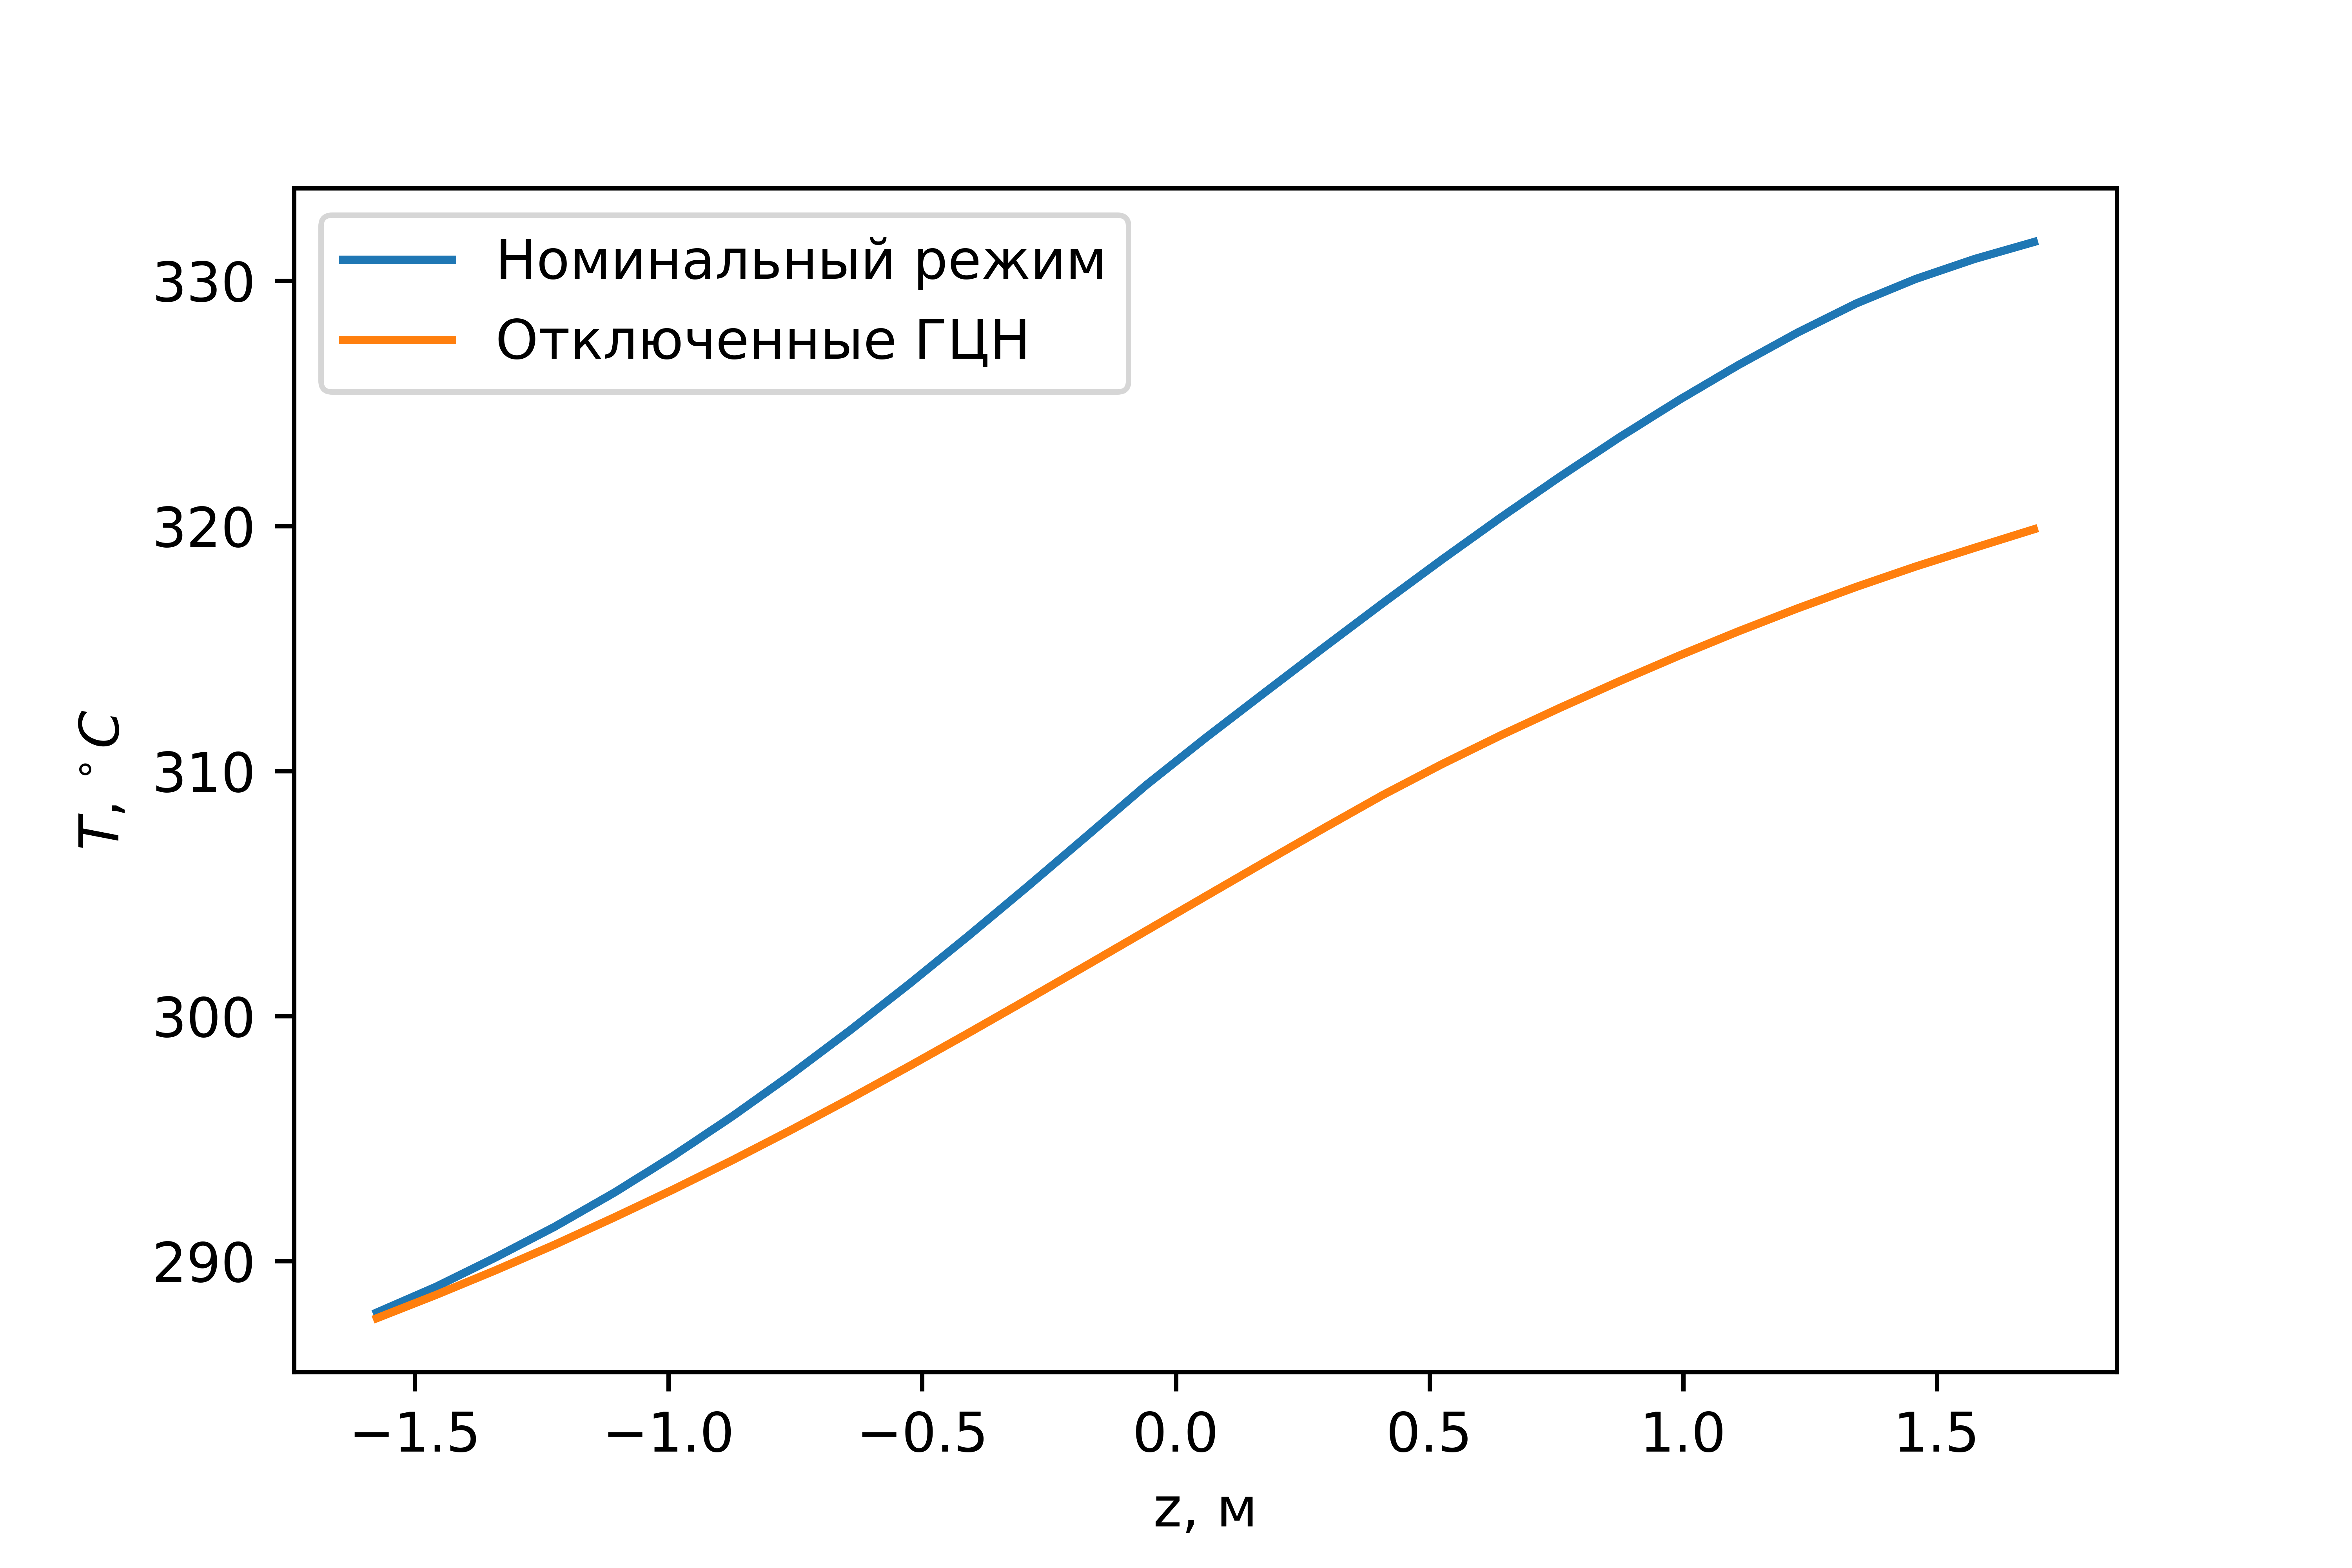
\includegraphics{treton_two_gcn_2_radius_T.png}
		\caption{Распределение температуры теплоносителя по высоте АЗ усредненное по семи ТВС вокруг центральной}
		\label{pic:treton-two-gcn-2-radius-T}
	\end{center}
\end{figure}

\section{Заключение}
В работе проводилось исследование работы РУ ВВЭР-1000 на номинальной, повышенной мощностях, а также при отключении одного и двух ГЦН с помощью програмного кода ТРЕТОН. По итогам были проанализированы поля температур соответствующих режимов, определены распределения основных теплогидравлических параметров. 

Для номинального режима работы проведено сравнение с теоретическим расчетом, в результате которого можно сделать вывод и применимости данной расчетной модели для исследуемой установки. Погрешность температур по сравнению с теоретическим расчетом составила 1\%.

Для работы реактора на повышенном уровне мощности была определена оптимальная в рамках используемой расчетной модели мощность в 105\% от номинальной, для которой были проанализированы температуры оболочек, топлива и теплоносителя. Были получены максимальные значения топлива, оболочек и теплоносителя 1502, 347.9, 334, $^\circ C$ соответственно. По результату анализа можно сделать вывод о возможности повышения мощности для реактора ВВЭР-1000 на 5\%, при которой температур насыщения не достигается за исключением возможного в рамках прогрешности расчетной модели программного комплекса ТРЕТОН пристеночного кипения в максимально нагруженных кассетах.

Для режимов с отключением ГЦН также проанализированы изменения теплогидравлических характеристик и перекосов полей температур. Для режима работы с одним отключенным ГЦН получены максимальные температуры топлива, оболочек и теплоносителя 1202, 335, 324.5 $^\circ C$ соответственно. Для режима с отключением двух гцн — 1068, 330, 321 $^\circ C$ соотвенно. По результатам анализа можно сделать вывод о возможности работы установки при отключении одного либо двух насосов.
